\documentclass{formato/UNIR}

%--- Parametros de entrada ---%
\titulo{Análisis de películas y creación de un sistema de recomendación}
\autor{Gonzalo Izaguirre de Diego}
\director{Yamila}
\fecha{Febrero 2020}
\ciudad{Zaragoza}
\universidad{Universidad Internacional de la Rioja (UNIR)}
\escuela{Departamento de ingeniería}
\master{Máster en Análisis y Visualización de Datos Masivos}
\tipoTesis{Trabajo Fin de Máster}

\keywords{Data Analysis, Data Visualization, Recomendation Engines} %Keywords en ingles
\keywordsEs{Análisis de Datos, Visualización de Datos, Sistemas de Recomendación} %Palabras clave en español


%--- Archivo de configuracion global ---%
\makeatletter
    \xdef\autorv{\@author}
    \xdef\titulov{\@title}
    \xdef\masterv{\@master}
    \xdef\fechav{\@date}
    \xdef\universidadv{\@universidad}
    \xdef\escuelav{\@escuela}
    \xdef\tipoTesisv{\@tipoTesis}
    \xdef\directorv{\@director}
    \xdef\ciudadv{\@ciudad}
\makeatother

%Referencias 
\usepackage{footmisc}
\usepackage{hyperref}
\hypersetup{
    pdftitle={\titulov},
    pdfauthor={\autorv},
    pdfsubject={\masterv},
    pdfpagemode={UseOutlines},
    bookmarksopen=true,
    bookmarksopenlevel=0,
    hypertexnames=false,
    colorlinks=true,
    pdfborder={0 0 0},
    citecolor=blue,
    linkcolor=blue,
    urlcolor=blue,
    pdfstartview={FitV},
    breaklinks=true
}

%Metadatos
\usepackage{hyperxmp}     
\AtBeginDocument{\hypersetup{pdfkeywords={\keywordsESv}}}


%Tablas (líneas horizonales toprule,bottomrule,midrule)
\usepackage{booktabs}

%Estructura del documento
\usepackage[toc,page,title,titletoc]{appendix}
\renewcommand*\appendixpagename{Apéndices}

%Idioma
\usepackage[spanish]{babel}
\addto\captionsspanish{\renewcommand{\tablename}{Tabla}}
\addto\captionsspanish{\renewcommand{\listtablename}{Índice de tablas}}

%Color azul UNIR
\usepackage[dvipsnames]{xcolor}
\definecolor{azul}{RGB}{81, 131, 187}
\def\azul{\color{azul}}
\def\an{\bfseries\azul}

%Márgenes UNIR
\RequirePackage{geometry}
\geometry{
	paper=a4paper,  
	left=3.5cm,
	right=1.5cm,
	top=2.5cm, 
	bottom=2.5cm,
	headheight=0.75cm,
	headsep=1.5cm,
	footskip=1.5cm,
	%showframe, % Ver marcos
}

%listings de codigo


\usepackage{listings}
\usepackage{xcolor}

\definecolor{codegreen}{rgb}{0,0.6,0}
\definecolor{codegray}{rgb}{0.5,0.5,0.5}
\definecolor{codepurple}{rgb}{0.58,0,0.82}
\definecolor{backcolour}{rgb}{0.95,0.95,0.92}

\lstdefinestyle{mystyle}{
    backgroundcolor=\color{backcolour},   
    commentstyle=\color{codegreen},
    keywordstyle=\color{magenta},
    numberstyle=\tiny\color{codegray},
    stringstyle=\color{codepurple},
    basicstyle=\ttfamily\footnotesize,
    breakatwhitespace=false,         
    breaklines=true,                 
    captionpos=b,                    
    keepspaces=true,                 
    numbers=left,                    
    numbersep=5pt,                  
    showspaces=false,                
    showstringspaces=false,
    showtabs=false,                  
    tabsize=2
}

\lstset{style=mystyle}

% Cabeceras y pies de página UNIR
\usepackage{lastpage}
\usepackage{fancyhdr}
\pagestyle{fancy}
\patchcmd{\chapter}{\thispagestyle{plain}}{\thispagestyle{fancy}}{}{}

\fancypagestyle{mainmatter}{%
    \fancyhead{}%
    \lhead{{\color{azul}\autorv}}%
    \chead{}%
    \rhead{\masterv}%
    \lfoot{{\color{azul}\titulov}}%
    \cfoot{}%
    \rfoot{\thepage\ %of \getpagerefnumber{LastPage}
    }}

\fancypagestyle{frontmatter}{%
    \fancyhead{}%
    \lhead{{\color{azul}\autorv}}%
    \chead{}%
    \rhead{\masterv}%
    \lfoot{{\color{azul}\titulov}}%
    \cfoot{}%
    \rfoot{\thepage}}

% Necesario para forzar encabezados y pies de página en la primera página de cada    
%\usepackage{etoolbox}      
\usepackage{setspace} % Espaciado entre líneas
\setstretch{1.5}
\usepackage[autostyle=true]{csquotes} % Referencias en UTF8

% Dependiendo del compilador se utilizan fuentes true type o fuentes convertidas (TFM)
\usepackage{array}
\usepackage{ifluatex,ifxetex}
\ifnum\ifluatex1\else\ifxetex1\else0\fi\fi
    =1 %
        % Fuentes comerciales TTF
    %Fuentes TFM UNIR: Arial, Georgia y Cambria
    \RequirePackage{fontspec}
    
    \setmainfont{Arial}[%
    Path=./formato/fuentes/,
    Extension=.ttf,
    UprightFont =*-Regular,
    BoldFont=*-Bold,
    ItalicFont=*-Italic,
    BoldItalicFont=*-BoldIt]
    
    \newfontfamily{\georgia}{Georgia}%
    [Path = ./formato/fuentes/,
    Extension = .ttf,
    UprightFont = *-Regular,
    BoldFont = *-Bold,
    ItalicFont =*-Italic,
    BoldItalicFont = *-BoldIt]
    
    \newfontfamily{\cambria}{Cambria}%
    [Path = ./formato/fuentes/,
    Extension = .ttf,
    UprightFont = *-Regular,
    BoldFont = *-Bold,
    ItalicFont =*-Italic,
    BoldItalicFont = *-BoldIt]
    
    \newcommand{\cambriamd}{\mdseries \cambria}
    \newcommand{\georgiamd}{\mdseries \georgia}
    \newcommand{\cambriab}{\bfseries \cambria}
    \newcommand{\georgiab}{\bfseries \georgia}

   
  
\else
    \renewcommand{\sfdefault}{arial}
\renewcommand{\familydefault}{\sfdefault}
\newcommand{\arialmd}{\usefont{T1}{arial}{m}{n}}
\newcommand{\arialb}{\usefont{T1}{arial}{b}{n}}
\newcommand{\arialit}{\usefont{T1}{arial}{m}{it}}
\newcommand{\arialbit}{\usefont{T1}{arial}{b}{it}}
\newcommand{\cambriamd}{\usefont{T1}{cambria}{m}{n}}
\newcommand{\cambriab}{\usefont{T1}{cambria}{b}{n}}
\newcommand{\cambriait}{\usefont{T1}{cambria}{m}{it}}
\newcommand{\cambriabit}{\usefont{T1}{cambria}{b}{it}}
\newcommand{\georgiamd}{\usefont{T1}{georgia}{m}{n}}
\newcommand{\georgiab}{\usefont{T1}{georgia}{b}{n}}
\newcommand{\georgiait}{\usefont{T1}{georgia}{m}{it}}
\newcommand{\georgiabit}{\usefont{T1}{georgia}{b}{it}}

\renewcommand{\mdseries}{\arialmd}
\renewcommand{\textmd}[1]{{\arial #1}}
\renewcommand{\bfseries}{\arialb}
\renewcommand{\textbf}[1]{{\arialb #1}}
\renewcommand{\itshape}{\arialit}
\renewcommand{\textit}[1]{{\arialit #1}}
\renewcommand{\normalfont}{\arialmd}
\renewcommand{\textnormal}[1]{{\arialmd #1}}


\fi


\usepackage{svg}

%--- Portada ---%
\renewcommand*{\maketitle}{%
    \begin{titlepage}%
        {\flushleft%
            {
\includegraphics[width=8.18cm]{./contenido/imagenes/logo-UNIR.pdf}}\par
        }%
        \vspace{1cm}
        \begin{table}[h!]
        \hyphenpenalty=10000
        \setlength\arrayrulewidth{2pt}
            \begin{tabularx}{14.5cm}{ L{0.074} !{\color{azul}\vline}  L{0.931} }
                & \\
                & \fontsize{14}{14}\selectfont \georgiab \universidadv\\
                & \\
                & \fontsize{18}{18}\selectfont \georgiab \escuelav \\
                & \\
                & \fontsize{14}{14}\selectfont  \georgiab\masterv \\
                & \\ & \\ & \\
                & \fontsize{42}{42}\selectfont \cambriamd \color{azul}   \titulov \\

            \end{tabularx}
        \end{table}
        \vspace{0.5cm}
        {\flushleft \fontsize{11}{11}\selectfont %
            \georgiab \tipoTesisv\par
                \vspace{0.3cm}
                Presentado por: \georgiamd \autorv \par
                \vspace{0.3cm}
                \georgiab Director: \georgiamd \directorv \par
                \vspace{2cm}
                {\color{azul}%
                \georgiab Ciudad: \georgiamd \ciudadv \par
                \georgiab Fecha: \georgiamd \fechav \par}
        }
    \end{titlepage}}

%---  Compilacion rapida ---%
% Para ahorrar tiempo de compilacion, comentar las secciones que no se quieran compilar
% Carácter % en frente de la sección.
\includeonly{
  contenido/TFM-00_Abstract,
  contenido/TFM-01_Introduccion,
  contenido/TFM-02_Objetivos_y_Metodologia,
  contenido/TFM-03_EstadoDelArte,
  contenido/TFM-04_Capitulo_X,
  contenido/TFM-09_Resultados,
  contenido/TFM-10_Bibliografia,
  contenido/TFM-11_Apendice_1,
%   contenido/TFM-11_Apendice_2 
}

%---------------------------------------------%
%           Inicio del documento
%---------------------------------------------%
\begin{document}
    %--- Paginas iniciales: portada,abstract,índice,lista de figuras y lista de tablas ---%. 
    \frontmatter
    \pagestyle{frontmatter}
        \maketitle          % Portada
        \tableofcontents    % Índice
        \clearpage
        \begin{abstract}[Resumen]
\par\vspace{-8.5cm}
En este proyecto analizamos la necesidad de utilizar sistemas de recomendación en el entorno tecnológico en el que vivimos. Con el tiempo, las bibliotecas de los servicios de vídeo online han ido creciendo de forma incesante. Con este incremento, cada vez se hace más difícil encontrar, a nivel individual, un contenido recomendable. Además, las plataformas de vídeo como Netflix o Amazon Prime Video están diseñadas para que se permanezca en ellas el máximo tiempo posible, haciendo que muchas veces no nos sean recomendados contenidos similares por estar en otras plataformas. En este proyecto, revisamos los diferentes tipos de sistemas de recomendación y sus implementaciones y creamos un sistema basado en contenido utilizando Python y Procesamiento del Lenguaje Natural para recomendar películas. Para realizar las recomendaciones se usarán las palabras clave de las películas y más metadatos disponibles. Se desarrollará una solución \textit{end to end}, no desarrollando únicamente el sistema sino también un entorno en el que podría ser utilizado. El resultado final consiste en paquete de Python que implementa una API integrada en un chatbot de Telegram que recomienda películas basándose en una aportada por el usuario.
\par\vspace{0.25cm}
\centering\textbf{Palabras clave: } \keywordsESv \par
\end{abstract}
\pagebreak
%Ingles
\begin{abstract}
In this project we discuss the need for recommendation systems in the technological enviroment we currently live on. The increase of the number of products available for the customers makes having a recommendation system a must for any online company looking for success. We review the different kinds of recommendation systems available and implement a content based one using Python and NLP to recommend films. An end to end solution will be developed, not only developing the system but also the enviroment in which it could be used. The final result consists on a Python  package that implements an API integrated in a Telegram chatbot. This chatbot recommends films based on one given by the user.
\par\vspace{0.25cm}
\centering\textbf{Keywords: } \keywordsv \par
\end{abstract}
  %Abtract
        \listoffigures      % Índice de imagenes
        \listoftables       % Índice de tablas
    
    %---    Cuerpo ---% 
    \mainmatter
    \pagestyle{mainmatter}
        %Incluir aqui todos los capitulos (carpeta contenido)
    	\chapter{Introducción}\label{chap:introduccion}
%Motivation

En los últimos años, con el crecimiento de plataformas online como Amazon, Netflix, YouTube y muchas otras, los contenidos disponibles para los usuarios han crecido de forma exponencial, habiéndose triplicado el número de películas lanzadas desde el año 2000 \cite{watson_2020} y multiplicado por 100 el número de horas subidas a YouTube cada minuto \cite{clement_2019}. \\

Hace no mucho tiempo si uno tenía que comprar un pequeño electrodoméstico para la cocina iba a una tienda especializada en ello. Si quería ver una película iba aun videoclub donde se le podían recomendar películas y alquilarlas, etc. Sin embargo, con el auge de Internet han aparecido plataformas que integran muchos de estos servicios. Amazon es un centro comercial virtual gigante en el que podemos encontrar desde alimentación hasta arte, pasando por tecnología, libros... e incluso ver películas en su plataforma. YouTube, por su parte, es una plataforma en la que los propios creadores de contenido suben de forma diaria $26$ millones de horas de vídeo al día y $1000$ millones de horas son visualizadas cada día por sus $2000$ millones de usuarios \cite{YoutubeStats}. Queda a la vista el hecho de que en los últimos años ha tenido lugar un cambio en el orden de magnitud de las plataformas de venta, pasando de pequeñas tiendas o cadenas nacionales a plataformas internacionales.\\

Uno de los grandes retos que estas plataformas han tenido que abordar es mantener a sus usuarios en ellas. Pongamos por ejemplo una persona en un ordenador con los miles de millones de vídeos que hay en YouTube, o delante de todos los contenidos que hay disponibles para visualizar en Netflix (1770 títulos en España \cite{Lovely2019}). El elegir qué contenido consumir puede ser una tarea de tal magnitud, que en ocasiones consigue ahuyentar al usuario. Por tanto, parece que ya no es suficiente con tener en la plataforma (tienda, antes; web, ahora) contenidos atractivos para el usuario, ni siquiera es ya suficiente con conseguir los usuarios acceder a la plataforma en cuestión dispuestos a usarla, sino que es vital que sea la plataforma quien les ayude a filtrar el contenido que puede ser de su agrado.\\

Por su parte, los hábitos de consumo de los usuarios también han evolucionado mucho en los últimos años. Desde escuchar la opinión de un producto de uno o varios vendedores y de su círculo más cercano hasta contar en la actualidad con grandes redes de encuentro entre usuarios donde diferentes productos son valorados y analizados. En un ejemplo concreto, una persona que quiera comprar un equipo de música para su hogar, hace unos años hubiera ido a una tienda cercana a su casa, hubiera preguntado al vendedor y, en base a la opinión del mismo y su presupuesto, hubiera realizado una elección. En la actualidad, podría buscar equipos de música en Amazon, que le serían ordenados según opiniones de otros usuarios, hubiera podido leer cientos de opiniones personales de compradores, visto análisis de expertos en YouTube, que analizarían de forma más objetiva las ventajas e inconvenientes de cada producto.\\

Se puede decir que con la llegada de estas plataformas ha llegado también la necesidad de ser capaz de orientar al consumidor dentro de las mismas, ya que de no hacerlo existe el riesgo de que el usuario se vea abrumado y no sea capaz de utilizarla. Tampoco puede decirse que el beneficio de ser capaz de realizar una recomendación al usuario sea sólo para él. La forma que tiene YouTube de recomendarte vídeos puede hacer que lo que iba a ser una visita de $10$ minutos se transforme en media tarde viendo vídeos y, en consecuencia, anuncios.\\

Nuestras intenciones y las de las plataformas online, no tienen por qué estar alineadas. Las plataformas actuales tienen motores de recomendación potentes, capaces de mantener a sus usuarios en la plataforma. Sin embargo, muchos los usuarios lo que desean es tratar de ver el contenido que mas les pueda gustar, independientemente de la plataforma en la que se encuentre. Las compañías usan un acercamiento que tiene en cuenta primero la plataforma, ya que recomiendan contenido que ellos tienen disponible. Mientras tanto, muchos usuarios pueden preferir un acercamiento que dé prioridad al contenido, sin importar la plataforma.\\

Ha quedado patente que en la actualidad se hace necesario disponer de sistemas que en base al contenido disponible y la opinión de los distintos usuarios sean capaces de recomendar productos de la plataforma \cite{Konstan2004}. La intención del proyecto es desarrollar un motor de recomendación que, sin disponer de la misma cantidad de datos que plataformas como Netflix, sea capaz de obtener unos resultados de satisfacción comparables, pero sin tener en cuenta la plataforma de visionado del contenido.


%%%           %%%
%  Objectives   %
%%%           %%%
\section{Objetivos del proyecto}\label{sec:objetivos}

Como se ha visto anteriormente, es muy beneficioso para las empresas que ofrecen productos online ser capaces de recomendar a sus usuarios otros productos a partir de los ya consumidos. Esto tiene, dos ventajas fundamentales:

\begin{itemize}
    \item ?La plataforma es capaz de orientar al usuario, de forma que se evita una posible fuga de usuarios a otras plataformas ante la ingente cantidad de productos a consumir.
    \item Una vez el usuario ha consumido un producto pueden serle recomendados otros relacionados, incrementando el número de productos consumidos por el usuario.
\end{itemize}

En este trabajo utilizaremos un conjunto de datos compuesto por información sobre películas, con la finalidad de construir un sistema de recomendación de películas que, partiendo de una película propuesta por el usuario, pueda recomendarle otras similares. La diferencia con el motor de búsqueda de plataformas como Netflix, es que estará disponible fuera de estas plataformas, en una app tan común como Telegram, y que recomendará películas de todo tipo, no solo las que estén en una determinada plataforma. Las preguntas a las que dará respuesta este TFE son:
\begin{itemize}
    \item \textquestiondown Es posible crear un sistema de recomendación usando recomendación basada en contenido? \textquestiondown Es Telegram una buena vía para realizar esta recomendación?
    \item \textquestiondown Prefiere el usuario recomendaciones que no tengan en cuenta la plataforma, pudiendo ver contenido más variado?
\end{itemize}

La forma en la que trataremos de mejorar los sistemas de plataformas como Netflix o Prime Video será, por tanto, en términos de riqueza del contenido y de posibilidad de recibir recomendaciones en cualquier situación, no solo dentro de estas plataformas.\\

El conjunto de datos utilizado\footnote{El conjunto de datos está disponible en \url{https://tinyurl.com/ypfdw8w}} posee metadatos sobre las películas, como palabras clave, presupuesto, puntuación de los usuarios... Información relevante y suficiente para poder implementar este sistema. Como puede deducirse, es necesario un soporte para este sistema que permita al usuario final poderlo utilizar. Lo habitual sería integrarlo con un trabajo de User Experience (UX) y que quedara, por tanto, integrado en la plataforma. En este caso no disponemos de una plataforma en la que integrar el sistema, por lo que se creará una API (que contendrá el sistema de recomendación) que podrá ser llamada por un bot de Telegram, de forma que recomiende películas a un usuario a partir de otra.\\

\begin{figure}[h]
    \centering
    \captionsetup{width=10cm}
    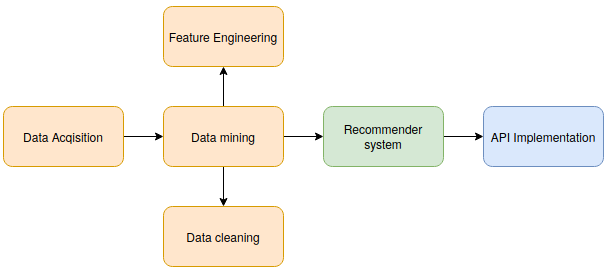
\includegraphics[width=12cm]{contenido/imagenes/initial.png}
    \caption{Metodología de trabajo abreviada. Proceso de tratado de la información para la creación del sistema de recomendación.}
    \label{fig:process}
\end{figure}

El proceso que se seguirá para la creación del sistema de recomendación se muestra en la \autoref{fig:process} y consistirá de los siguientes pasos:
\begin{enumerate}
    \item Adquisición de los datos y limpieza de los mismos.
    %\item Análisis preliminar avanzado de los datos.
    \item Creación del sistema de recomendación.
    \item Creación de la API e integración en el bot de Telegram.
\end{enumerate}
%%%                  %%%
% Document structure   %
%%%                  %%%
\section{Estructura de la memoria}\label{sec:estructura}

El trabajo, como se ha descrito en los capítulos anteriores, tiene como objetivo la creación de un sistema de recomendación de películas, aunque se tratará de incluir en el mismo el flujo \textit{end to end} de tratamiento de la información. El trabajo se estructurará en diferentes capítulos, conteniendo cada uno de ellos una de las partes del flujo. Los capítulos que se incluirán en este trabajo serán los siguientes:

\begin{itemize}
    \item \autoref{chap:recom}: Sistemas de recomendación. Se realizará una explicación de la teoría que existe tras estos sistemas y los diferentes tipos que existen. Se creará el sistema de recomendación.
    \item \autoref{chap:adq}: Estructura de los datos a utilizar y preprocesado de los mismos. En este capítulo se realizará una presentación y explicación de los datos de los que se dispone, de forma que se entiendan los siguientes pasos seguidos.
    %\item \textit{Preliminary Data Analysis}. Caso de uso de análisis de datos para resolución de preguntas de negocio. %Al trabajar con un conjunto de datos siempre es importante realizar un análisis previo, de forma que pueda %entenderse la estructura de los mismos. También se verá la utilidad de disponer de un conjunto de datos %relativamente grande a la hora de responder a preguntas que pueden surgir en relación con la informacion contenida %en los mismos.
    
    \item \autoref{chap:api}: Integración del sistema en una API y creación de un chatbot. Es importante que nuestro sistema de recomendación sea explotable por los usuarios, de nada sirve tener un buen sistema de recomendación si no puede ser usado. Se explicará la creación de un bot de Telegram y cómo crear una API que pueda ser llamada por el bot.
    \item \autoref{chap:resultados}: Resultados. En este capítulo se detallará la metodología seguida para realizar una evaluación del sistema construido en el trabajo y se mostrarán los resultados obtenidos.
    \item \autoref{chap:futuro}: Conclusiones y trabajo futuro. Finalmente, se realizará un repaso de lo desarrollado en el trabajo y se propondrán puntos en los que mejorar el sistema que no hayan podido implementarse por algún motivo.
\end{itemize}

\section{Alcance del trabajo desarrollado}\label{sec:trabajodesarrollado}

En esta memoria, se trata de solventar el problema que se ha comentado en las secciones anteriores. Las plataformas de contenido disponen de sistemas de recomendación potentes, pero con una limitación de origen: solo recomiendan contenido de sus plataformas. Esto hace que si vemos una película concreta en una plataforma y esta nos recomienda otra, es posible que haya mejores recomendaciones que la plataforma en cuestión no esté realizando debido a que no dispone de ese contenido.\\ 

Tal y como se verá en el \autoref{chap:recom}, un tipo de motores de recomendación son los motores basados en contenido. Estos motores se basan en características intrínsecas de las películas y no tanto en las opiniones atómicas de los usuarios. En la solución propuesta en este trabajo, las palabras clave que describen una película son la parte central de la recomendación. Esta elección se ha realizado principalmente por los datos disponibles, ya que los temas de una película, su año de producción o la opinión media de los usuarios son datos relativamente abiertos, mientras que las opiniones concretas de cada usuario son algo propiedad de las plataformas en las que se realizan estas valoraciones, por lo que no tenemos acceso a estos datos.\\ 

Para realizar la recomendación y una vez se ha limpiado el dataset, las películas se distribuyen en un espacio vectorial de keywords y se seleccionan en base a una distancia las más próximas a la película dada. Una vez se tienen las películas más cercanas a la película dada, se establece una heurística que puntúa cada una de estas películas en función de su puntuación, su año de producción y el ratio entre votos e ingresos. Esta heurística trata de, una vez se han seleccionado las películas candidatas a ser recomendadas, tratar de escoger de entre ellas las que probablemente prefiera el usuario. Por ejemplo, creemos que si tras ver una película de Harry Potter se nos recomienda una de magia similar pero del año 1950 es probable que el usuario sea reacio a escogerla.\\

Una de las principales ventajas de nuestro motor de recomendación, es la forma en la que se ha implementado. Al ser un motor agnóstico en términos de plataforma (ya que simplemente tiene datos de las películas y su puntuación en IMDB), necesitábamos un sitio desde el que pudiera ser explotado. De entre todos los posibles, hemos elegido implementarlo en un bot de Telegram, ya que Telegram es una plataforma con una gran expansión y además multiplataforma. Consideramos que la mayoría de usuarios tendrán a mano un dispositivo móvil cuando estén viendo películas, por lo que en cualquier momento pueden escribir un título al bot y éste les enviará las recomendaciones obtenidas.\\

Además, nuestro motor (y en general los motores basados en contenido) tiene una ventaja principal, y es que puede ser actualizado fácilmente con la llegada de nuevas películas a la cartelera. Dado que la información principal que utilizamos son las palabras clave, no necesitamos que un gran número de usuarios haya visto la película en cuestión para que tengamos la información suficiente para recomendar esa nueva película. Esto hace que sea un modelo especialmente beneficioso para que los usuarios puedan descubrir películas menos conocidas que puedan ser de su agrado.\\

Uno de los problemas que suelen tener los motores de recomendación basados en contenido es que en muchas ocasiones recomiendan elementos demasiado similares. Esto se entiende mejor con un ejemplo: imaginemos que nuestra última compra en Amazon es un teclado de ordenador. Si Amazon nos recomendase los productos más parecidos, probablemente nos recomendase otros teclados. Normalmente, cuando hemos comprado un teclado lo último que necesitamos es otro. Las recomendaciones serían, en este caso, tan similares que no serían de utilidad. Sin embargo, consideramos que como nuestro sistema sirve para recomendar películas, este problema se ve mitigado por el mero hecho de que no hay películas tan similares entre sí como productos en Amazon, por ejemplo.


    

        
\chapter{Objetivos y Metodología}\label{chap:objetivos}

Este trabajo tiene como objetivo presentar un caso de uso de las herramientas estudiadas en el máster. Como se ha descrito en capítulos anteriores, el caso de uso elegido es partir de fuentes de datos relacionadas con películas y desarrollar un \textbf{sistema de recomendación} que sea capaz de dar al usuario películas similares a las dadas por él.\\

Para ello se realizará un \textbf{análisis de los datos} y una presentación teórica de los diferentes modelos que existen para crear un sistema de recomendación. Finalmente, se escogerá una técnica concreta en función de sus ventajas y los datos disponibles y se implementará. Para que pueda ser usado en un entorno más productivo y fuera de un ordenador particular, se integrará en el flujo un chatbot que pueda recibir la información del usuario, procesarla, y darle recomendaciones haciendo llamadas a una \textbf{API} que será creada.



%--- Genereal Objectives ---%
\section{Objetivos Generales}\label{sec:objgenerales}

Crear un sistema de recomendación de películas agnóstico a la plataforma en la que el contenido está disponible y utilizable en cualquier entorno. Con este fin, se usarán los datos disponibles en \cite{kaggle}\\

En el mundo actual los usuarios disponen de una gran cantidad de recursos a consumir cuando entran a una plataforma como YouTube o Netflix. Por tanto, se hace necesario que las plataformas sean capaces de entender sus \textbf{gustos y preferencias} para que el cliente consuma la mayor cantidad de contenido posible. En este trabajo se explora la vía de creación de un sistema de recomendación basado en contenido que, a partir de modelos de lenguaje sea capaz de entender el contenido de cada una de las películas y a partir de una preferencia dada por el usuario, le pueda recomendar otras películas similares para ver. Además, destruirá la barrera de la plataforma que imponen los sistemas embebidos dentro de estas. El sistema desarrollado recomendará sin tener en cuenta dónde está disponible el contenido, con el fin de ampliar los horizontes del usuario.\\

Como se verá más adelante, en el \autoref{chap:recom}, existen diferentes tipos de sistemas de recomendación. En este trabajo nos centraremos en sistemas basados en contenido, dado que tienen ventajas como su capacidad para recomendar productos nuevos y la no necesidad de información del usuario. Además, la información sobre las películas es más sencilla de obtener en la red.\\

Explicado esto, este trabajo se engloba dentro de los trabajos de Tipo 2 (desarrollo de software). Se realizará un desarrollo de una solución \textit{end to end} al problema de la recomendación de contenidos a usuarios. Desde la recopilación de datos y metadatos sobre películas, hasta la creación de la interfaz a través de la que el usuario final podrá hacer solicitudes al sistema creado y obtener recomendaciones.\\

Además, se realizará una revisión de los diferentes sistemas de recomendación existentes en la actualidad y su aparición en los últimos años.\\

%Finalmente, creemos necesario realizar un análisis de los datos que se utilizaran, previo a la creación del sistema de recomendación. En el %campo de la Ciencia de Datos se considera una buena práctica la realización de un análisis de los datos de forma previa a la creación del %sistema de recomendación en sí. Además de este análisis preliminar, mostraremos cómo el disponer de un conjunto lo suficientemente extenso de %datos puede servir para responder preguntas sobre los usuarios, que pueden ayudar al desarrollo del negocio.\\


%--- Specific Objectives ---%
\section{Objetivos Específicos}\label{sec:objespecificos}

Una vez descritos los objetivos generales del trabajo que se desarrollará, se hace necesario desgranarlos en una serie de objetivos más específicos que puedan ser más fácilmente analizados y desarrollados y para los que pueda establecerse un grado de consecución.

\begin{itemize}
    \item Conocer las fuentes de datos disponibles, el formato de los datos de películas y actores y sus posibilidades de explotación.
    \item Describir los datos disponibles y analizar los datos para sacar conclusiones sobre los mismos.
    %\item \textbf{IDENTIFICAR} tendencias a partir de los datos y \textbf{RESPONDER} a partir de ellos a preguntas que puedan surgir.
    \item Desarrollar el sistema de recomendación de películas que permita a los usuarios obtener recomendaciones a partir de una película dada..
    \item Integrar la solución desarrollada en un entorno API-bot que pueda ser usada por usuarios finales.
    \item Verificar la usabilidad de la solución y evaluar el rendimiento de la misma.
    \item Identificar las flaquezas del sistema y los puntos de mejora para proponer próximos pasos.
\end{itemize}

%--- Work Methodology ---%
\section{Metodología de Trabajo}\label{sec:metodología}

En este trabajo, se ha utilizado una metodología definida de forma inicial, aunque posteriormente se han tenido que ir realizando adaptaciones de la misma a medida que se desarrollaba el mismo.\\

En primer lugar, hay se definió de forma concreta el problema que se quería resolver y se realizó una investigación bibliográfica con la finalidad de conocer los diferentes sistemas de recomendación que existen, de forma que pudiéramos definir correctamente el tipo de sistema que se quería utilizar y los datos necesarios.\\

Partiendo del problema descrito en la introducción, se buscó un conjunto de datos que hiciera posible dar una solución al problema. El conjunto de datos disponible está disponible en \cite{kaggle}.\\

Una vez encontrados unos datos con los que trabajar, se definieron los pasos a seguir para la implementación del proyecto y la resolución del problema:
\begin{enumerate}
    \item Limpieza de los datos: En un proyecto de análisis de datos real, es una fase imprescindible. En esta fase se revisan los datos originales, se borran los datos incorrectos y se tratan los valores incorrectos o faltantes. Las herramientas a utilizar en esta etapa serán principalmente Python y la librería Pandas.
    \item Preprocesamiento de los datos: Una vez se hayan limpiado los datos, será necesario realizar un preprocesamiento de los mismos para que sirvan de entrada al sistema de recomendación, fase en la que se usará Python y librerías de procesamiento de lenguaje natural si fuera necesario.
    \item Construcción del sistema de recomendación: Tras la investigación bibliográfica y el preprocesamiento de los datos, se construirá el sistema de recomendación en sí. El objetivo es poder dar 3 recomendaciones de películas dada una de entrada, que pueda tener faltas de ortografía, de forma que el sistema sea más flexible.
    \item Integración del sistema en una API: Desde el principio, la intención ha sido crear un sistema usable y desde una perspectiva \textit{end to end}. En muchas ocasiones este tipo de trabajos se quedan en una mera investigación bibliográfica y teórica. Sin embargo, la intención es que el sistema sea realmente usable por todo el mundo que lo desee. En esta fase se valorarán las diferentes alternativas para proveer de una interfaz al sistema creado, generando un servicio web desde el que puedan realizarse recomendaciones.
\end{enumerate}
        \chapter{Estado del Arte}\label{chap:estadodelarte}
Donec \ref{tab:table1} vestibulum purus in aliquet molestie. Quisque id consectetur purus. Orci varius natoque penatibus et magnis dis parturient montes, nascetur ridiculus mus. Nam at ipsum vitae ipsum venenatis mollis. Donec id orci in eros accumsan dignissim. Vivamus laoreet purus a velit suscipit molestie. Proin arcu erat, aliquet nec augue quis, ultrices placerat magna. Sed ut sodales odio, at interdum mauris. Nullam consectetur semper odio, et condimentum augue volutpat quis. Maecenas nec purus ornare, bibendum turpis at, placerat libero.\par

Nunc  id mollis ex, aliquet consectetur dolor. In consequat turpis a magna commodo congue. Donec nec elit posuere, placerat ex id, elementum mi. Phasellus sed rhoncus est. Sed mollis eros non ante hendrerit condimentum. Sed sem nulla, bibendum in nisi vitae, mollis finibus neque. Proin auctor lacus nunc, vel venenatis orci rutrum ut. Quisque lacinia ut tellus non maximus. Phasellus elementum tincidunt lorem sit amet maximus. Nunc venenatis, risus sit amet tincidunt ornare, felis sem facilisis augue, quis dignissim lorem leo eu libero. In quis justo id arcu eleifend blandit. Ut tortor libero, tempor nec vestibulum at, malesuada sit amet ipsum.\par

Fusce vitae sem ligula. Nunc vulputate enim ut eros pretium, eget pellentesque nibh ullamcorper. Ut commodo enim nec sapien hendrerit tincidunt. Aenean pulvinar purus nisl, at congue lectus pharetra nec. Phasellus faucibus lacus at est vestibulum commodo. Sed consequat, augue id faucibus dapibus, urna est scelerisque turpis, ut luctus massa lacus eu sem. Aliquam lobortis massa mauris, a finibus eros gravida et.\par

\begin{table}[h]
    \begin{tabularx} {13cm} {lcccccc|c} \cmidrule[\heavyrulewidth]{2-8} 
    &\multicolumn{2}{c}{Phasellus Quisque } &\multicolumn{2}{c}{Aenean} &\multicolumn{2}{c|}{Curabitur} &Aliquam\\ \cline{2-7}
                                    &Aliquam    &Lobortis    &Aliquam    &Lobortis    &Aliquam    &Lobortis    &Lobortis \\ \cmidrule{1-8}
                Elementum	            &0          &0	        &0          &0	        &0          &0          &\azul0\\
                Libero	            &0          &0	        &33         &\n1  	    &1          &0          &\an1\\
                Vulputate	            &7          &0	        &6          &\n1        &1          &0          &\an1\\
                Proin	            &0          &0	        &0          &0          &0          &0          &\azul0\\  
                Strategy Map        &0          &0	        &1          &0          &1          &\an1       &\an1\\ 
                Tincidunt               &0          &0	        &0          &0  	    &0          &0          &\azul0\\
                Bibendum	            &0          &0	        &3          &0  	    &0          &0          &\azul0\\
                Accumsan            &1          &0	        &4          &0  	    &1          &0          &\azul0\\
                Commodo           &3          &\n1        &4          &0  	    &4          &\n3        &\an4\\
                Tortor                 &1          &0	        &3          &0  	    &2          &0          &\azul0\\
                Vitae                 &0          &0	        &17         &0 	        &18         &\n2        &\an2\\ \cmidrule[\heavyrulewidth]{1-8}
    \end{tabularx}
    \caption{Donec nec auctor mi. Cras ante turpis.}
    \label{tab:table1}
\end{table}

Nulla semper massa quis pretium ullamcorper. Nulla id pulvinar purus. In porta ultrices tincidunt. Donec gravida semper eros, auctor fringilla purus tristique vel. Donec vitae urna sit amet purus pharetra congue. Proin condimentum nisl id ultricies ultrices. In hac habitasse platea dictumst. Cras congue bibendum nunc. Phasellus sagittis facilisis aliquam. In feugiat odio quis mauris luctus imperdiet.\par

Praesent odio diam, mattis eu lacus et, elementum vulputate enim. Etiam vestibulum et lectus et vestibulum. Cras vel neque ac dolor sodales elementum. Duis posuere est sollicitudin faucibus elementum. Donec non sollicitudin diam. Curabitur tincidunt justo id sapien lacinia accumsan. Donec eget odio vitae felis luctus elementum a sit amet purus. Curabitur ac lectus vitae lectus iaculis laoreet. \par
        \chapter{Vivamus non pellentesque}\label{chap:vivamus}
Mauris ullamcorper ante sed rhoncus suscipit. Nunc ultrices, purus a tristique tincidunt, tellus sem suscipit leo, vel vulputate libero libero non elit. Etiam tristique libero elit, ut interdum ligula rhoncus sed. Quisque nec imperdiet purus, ut malesuada tortor. Etiam posuere eros sed sem sagittis, sit amet sagittis risus porttitor. Nulla vehicula enim maximus sapien dictum pharetra. Proin vehicula diam nec tristique tincidunt. Nulla sagittis nulla in convallis consectetur. Interdum et malesuada fames ac ante ipsum primis in faucibus. Nunc ultricies quam a leo molestie, in rhoncus turpis hendrerit. Phasellus vulputate risus sit amet metus volutpat, id iaculis erat tincidunt. In hac habitasse platea dictumst. Vestibulum non augue ullamcorper, mollis tellus at, aliquam risus. Ut congue malesuada lectus, nec congue massa dignissim a. Proin et facilisis massa, nec porttitor tellus. Etiam id feugiat ipsum, vitae mollis nunc.\par

Nunc sed magna eu orci malesuada scelerisque quis non metus. Maecenas vulputate leo quis sem lacinia pretium. Ut venenatis velit venenatis metus finibus consectetur. Integer ornare magna mi, sed semper nibh hendrerit a. Sed vitae molestie lorem, ut mattis felis. Duis eget mauris vehicula enim tincidunt mollis eget ut arcu. Vivamus non pellentesque mi, quis facilisis nisl. Sed sit amet venenatis urna. Mauris elit purus, facilisis eu ipsum imperdiet, placerat hendrerit ligula. Mauris ut dolor ipsum. Nunc id varius justo, et fringilla dolor.\par

Suspendisse ultricies nisi enim, eget consectetur neque iaculis et. Cras dignissim orci nec elit dignissim convallis. Mauris vitae neque nec enim semper viverra vitae a felis. Proin eu libero at nisl porttitor dictum. Maecenas nec hendrerit elit. Nulla auctor nec arcu eu dapibus. Suspendisse et leo eu sem dignissim mattis. Maecenas consectetur libero ex, nec posuere ante gravida a. Orci varius natoque penatibus et magnis dis parturient montes, nascetur ridiculus mus. Morbi dictum mollis metus nec tincidunt. In ullamcorper eros sollicitudin tempus vehicula.\par

Suspendisse quis ligula quam. Phasellus eu eros eu metus pellentesque pharetra vitae tempor risus. Nam lectus urna, feugiat et viverra nec, commodo eu metus. Fusce laoreet convallis nisi ac ultricies. Proin laoreet lacinia turpis non porttitor. Vestibulum tincidunt nisi et justo pulvinar, a finibus metus fringilla. Sed tincidunt, erat vel placerat mollis, velit nibh elementum felis, ut pellentesque nunc ligula ac orci. Sed semper molestie nisl, eget sagittis quam dictum vel. Nam tincidunt justo quis ex gravida egestas. Suspendisse potenti.\par

Proin sagittis luctus dolor, eu aliquam risus mollis eu. Mauris commodo est sed enim maximus, sit amet fringilla ipsum molestie. Duis ullamcorper volutpat suscipit. Suspendisse et nisl dolor. Sed ac sollicitudin ante. Fusce nec velit rutrum, iaculis neque non, pretium ante. Donec sed metus ex. Nullam est nulla, viverra vitae lacinia vel, hendrerit non purus. Phasellus id nibh vitae enim viverra convallis. Ut id tincidunt lorem. Suspendisse porta, risus non semper consectetur, lorem justo luctus justo, ut venenatis nisi felis id arcu. Duis hendrerit tellus in vestibulum convallis. Integer pharetra rhoncus erat. Sed auctor lacinia erat suscipit pretium. Nunc sed nisi rhoncus est auctor elementum ut a lorem. Mauris blandit lacus in consectetur vulputate.\par

Sed at sodales metus, a varius dolor. Vivamus sodales tellus vitae metus tristique dignissim. Nullam magna ex, blandit id vulputate vitae, suscipit at arcu. Ut lacinia vulputate lacus quis venenatis. Quisque eu lacinia lectus. Aliquam a est ut tortor vehicula posuere sagittis a neque. Mauris id sollicitudin mi. Vestibulum et auctor metus. Donec consequat elit at lectus dictum, lacinia elementum odio luctus. Curabitur a ante ipsum. Quisque eleifend erat eu porttitor imperdiet.\par

Quisque eget ultrices ex. Nunc accumsan, ipsum id viverra malesuada, nisl velit semper neque, eu consectetur dolor nisl vitae tellus. Nam iaculis nisl quis tortor accumsan semper. Sed imperdiet a libero ut ornare. Sed mattis ipsum nec aliquet porta. Maecenas blandit nibh a ante placerat, sit amet aliquet leo sodales. Sed ut velit non ligula pharetra tristique. Curabitur eget turpis in felis tristique consectetur ac id elit. Curabitur tincidunt nulla erat, vitae placerat velit congue non. Mauris ut velit nec arcu hendrerit tristique. Vivamus molestie, est quis posuere sollicitudin, quam nibh dictum dui, ut convallis tortor libero in mauris. Etiam ac molestie arcu. Duis nec mi dapibus, pharetra dolor at, consequat massa. Pellentesque tempor leo et lacus placerat tempus. Suspendisse faucibus sagittis neque ut aliquam. Nullam rutrum eleifend odio, varius tincidunt orci feugiat sit amet.\par


        \include{contenido/TFM-05_SeleccionAtrib}
        \chapter{Conclusiones y trabajo futuro}\label{chap:resultados}
Este último bloque (habitualmente un capítulo; en ocasiones, dos capítulos complementarios) es habitual en todos los tipos de trabajos y presenta el resumen final de tu trabajo y debe servir para informar del alcance y relevancia de tu aportación.\par

Suele estructurarse empezando con un resumen del problema tratado, de cómo se ha abordado y de por qué la solución sería válida.
Es recomendable que incluya también un resumen de las contribuciones del trabajo, en el que relaciones las contribuciones y los resultados obtenidos con los objetivos que habías planteado para el trabajo, discutiendo hasta qué punto has conseguido resolver los objetivos planteados.\par

Finalmente, se suele dedicar una última sección a hablar de líneas de trabajo futuro que podrían aportar valor añadido al TFM realizado. La sección debería señalar las perspectivas de futuro que abre el trabajo desarrollado para el campo de estudio definido. En el fondo, debes justificar de qué modo puede emplearse la aportación que has desarrollado y en qué campos.

\begin{table}[H]
\centering
\begin{tabular}{llrr}
\toprule
{} &           column\_name &  missing\_count &  filling\_factor \\
\midrule
0  &              homepage &           3091 &           35.64 \\
1  &               tagline &            844 &           82.43 \\
2  &               country &            174 &           96.38 \\
3  &          actor\_3\_name &             93 &           98.06 \\
4  &              language &             86 &           98.21 \\
5  &          actor\_2\_name &             63 &           98.69 \\
6  &          actor\_1\_name &             53 &           98.90 \\
7  &         director\_name &             30 &           99.38 \\
8  &              overview &              3 &           99.94 \\
9  &              duration &              2 &           99.96 \\
10 &            title\_year &              1 &           99.98 \\
11 &          release\_date &              1 &           99.98 \\
12 &       num\_voted\_users &              0 &          100.00 \\
13 &          vote\_average &              0 &          100.00 \\
14 &           movie\_title &              0 &          100.00 \\
15 &                budget &              0 &          100.00 \\
16 &      spoken\_languages &              0 &          100.00 \\
17 &  production\_countries &              0 &          100.00 \\
18 &  production\_companies &              0 &          100.00 \\
19 &            popularity &              0 &          100.00 \\
20 &        original\_title &              0 &          100.00 \\
21 &         plot\_keywords &              0 &          100.00 \\
22 &                    id &              0 &          100.00 \\
23 &                genres &              0 &          100.00 \\
24 &                status &              0 &          100.00 \\
25 &                 gross &              0 &          100.00 \\
\bottomrule
\end{tabular}
\caption{Dimensiones de los datos de entrenamiento utilizados en \textbackslash{}cite\{Li2018\}}
\label{tab:datasets}
\end{table}

    %--- Apéndices y bibliografia ---%
    \cleardoublepage
\phantomsection
\addcontentsline{toc}{chapter}{Bibliography}
\printbibliography
    \begin{appendices}
        %Incluir aqui todos los apendices (carpeta contenido).
        \chapter{Notebook completo utilizado para la creación del sistema de recomendación}\label{app:notebook}




    \section{\texorpdfstring{\textbf{Film recommendation
engine}}{Film recommendation engine}}\label{film-recommendation-engine}

\emph{Gonzalo Izaguirre (diciembre 2019)} \_\_\_

El objetivo de este notebook es crear un motor de recomendación a partir
del contenido del fichero \texttt{movie\_metadata.csv}.Este dataset
contiene alrededor de 5000 películas y series, y su descripción ha sido
recogida de la base de datos de IMDB. Basicamente, el sistema funcionará
de la siguiente forma: después de que el usuario haya introducido el
nombre de una película que le haya gustado, el sistema seleccionará del
conjunto total 5 películas que agradarán al usuario al ser similares.
This dataset contains around 5000 movies and TV series, and their
description has been retrieved from the public IMDB database. Existen
tres tipos de filtros colaborativos: - Sistemas
\textbf{popularity-based}: los más simples de implementar, aunque los
más impersonales - Sistemas \textbf{content-based}: La recomendación se
basa en la descripción del producto - Sistemas \textbf{collaborative
filtering}: datos de diferentes usuarios dan recomendaciones basadas en
similaridades entre usuarios.

In the current case, since the dataset only describe the content of the
films and TV series, collaborative filtering is excluded and I will thus
build an engine that uses both the content and the popularity of the
entries.

En este caso, dado que el conjunto de datos solo describe el contenido
de las películas, no puede aplicarse el filtrado colaborativo. Se creará
un motor que usará tanto el contenido como la popularidad de las
entradas. \_\_\_ El notebook se organiza de la siguiente manera:

\textbf{1. Exploración} - 1.1 Keywords - 1.2 Factor de completitud:
Valores Faltantes - 1.3 Películas por año - 1.4 Géneros

\textbf{2. Limpieza} - 2.1 Entradas duplicadas - 2.2 Limpieza de
keywords * 2.2.1 Agrupamiento por lexema * 2.2.2 Agrupamiento por
sinónimos - 2.3 Correlaciones - 2.4 Valores faltantes * 2.4.1 Años
faltantes * 2.4.2 Extrayendo keywords del título * 2.4.3 Completado de
datos mediante regresión

\textbf{3. Recommendation Engine} - 3.1 Funcionamiento básico del motor
* 3.1.1 Similaridad * 3.1.2 Popularidad - 3.2 Definicion de las
funciones del motor de recomendación - 3.3 Realizando recomendaciones
interesantes - 3.4 Ejemplo de recomendación

\textbf{4. Conclusión: posibles mejoras y puntos a concretar}

    \begin{center}\rule{0.5\linewidth}{\linethickness}\end{center}

\subsection{1. Exploración}\label{exploraciuxf3n}

Se cargan todos los paquetes y el conjunto de datos. Se da información
sobre los tipos de las columnas y los datos faltantes.

    \begin{tcolorbox}[breakable, size=fbox, boxrule=1pt, pad at break*=1mm,colback=cellbackground, colframe=cellborder]
\prompt{In}{incolor}{1}{\hspace{4pt}}
\begin{Verbatim}[commandchars=\\\{\}]
\PY{c+c1}{\PYZsh{} new code block}
\PY{k+kn}{import} \PY{n+nn}{json}
\PY{k+kn}{import} \PY{n+nn}{pandas} \PY{k}{as} \PY{n+nn}{pd}
\end{Verbatim}
\end{tcolorbox}

    \begin{tcolorbox}[breakable, size=fbox, boxrule=1pt, pad at break*=1mm,colback=cellbackground, colframe=cellborder]
\prompt{In}{incolor}{2}{\hspace{4pt}}
\begin{Verbatim}[commandchars=\\\{\}]
\PY{c+c1}{\PYZsh{} new code block}
\PY{k}{def} \PY{n+nf}{load\PYZus{}tmdb\PYZus{}movies}\PY{p}{(}\PY{n}{path}\PY{p}{)}\PY{p}{:}
    \PY{l+s+sd}{\PYZdq{}\PYZdq{}\PYZdq{}}
\PY{l+s+sd}{    Función utilizada para cargar el dataset de las películas. Se transforma a fecha el campo de fecha de salida}
\PY{l+s+sd}{    y se cargan como listas los campos que están guardados como json.}

\PY{l+s+sd}{    Args:}
\PY{l+s+sd}{        path: Ruta hasta el archivo de tmdb\PYZus{}5000\PYZus{}movies.csv}

\PY{l+s+sd}{    Returns:}
\PY{l+s+sd}{        Dataframe de pandas con la información del csv}
\PY{l+s+sd}{    \PYZdq{}\PYZdq{}\PYZdq{}}
    \PY{n}{df} \PY{o}{=} \PY{n}{pd}\PY{o}{.}\PY{n}{read\PYZus{}csv}\PY{p}{(}\PY{n}{path}\PY{p}{)}
    \PY{n}{df}\PY{p}{[}\PY{l+s+s1}{\PYZsq{}}\PY{l+s+s1}{release\PYZus{}date}\PY{l+s+s1}{\PYZsq{}}\PY{p}{]} \PY{o}{=} \PY{n}{pd}\PY{o}{.}\PY{n}{to\PYZus{}datetime}\PY{p}{(}\PY{n}{df}\PY{p}{[}\PY{l+s+s1}{\PYZsq{}}\PY{l+s+s1}{release\PYZus{}date}\PY{l+s+s1}{\PYZsq{}}\PY{p}{]}\PY{p}{)}\PY{o}{.}\PY{n}{apply}\PY{p}{(}\PY{k}{lambda} \PY{n}{x}\PY{p}{:} \PY{n}{x}\PY{o}{.}\PY{n}{date}\PY{p}{(}\PY{p}{)}\PY{p}{)}
    \PY{n}{json\PYZus{}columns} \PY{o}{=} \PY{p}{[}\PY{l+s+s1}{\PYZsq{}}\PY{l+s+s1}{genres}\PY{l+s+s1}{\PYZsq{}}\PY{p}{,} \PY{l+s+s1}{\PYZsq{}}\PY{l+s+s1}{keywords}\PY{l+s+s1}{\PYZsq{}}\PY{p}{,} \PY{l+s+s1}{\PYZsq{}}\PY{l+s+s1}{production\PYZus{}countries}\PY{l+s+s1}{\PYZsq{}}\PY{p}{,} \PY{l+s+s1}{\PYZsq{}}\PY{l+s+s1}{production\PYZus{}companies}\PY{l+s+s1}{\PYZsq{}}\PY{p}{,} \PY{l+s+s1}{\PYZsq{}}\PY{l+s+s1}{spoken\PYZus{}languages}\PY{l+s+s1}{\PYZsq{}}\PY{p}{]}
    \PY{k}{for} \PY{n}{column} \PY{o+ow}{in} \PY{n}{json\PYZus{}columns}\PY{p}{:}
        \PY{n}{df}\PY{p}{[}\PY{n}{column}\PY{p}{]} \PY{o}{=} \PY{n}{df}\PY{p}{[}\PY{n}{column}\PY{p}{]}\PY{o}{.}\PY{n}{apply}\PY{p}{(}\PY{n}{json}\PY{o}{.}\PY{n}{loads}\PY{p}{)}
    \PY{k}{return} \PY{n}{df}


\PY{k}{def} \PY{n+nf}{load\PYZus{}tmdb\PYZus{}credits}\PY{p}{(}\PY{n}{path}\PY{p}{)}\PY{p}{:}
    \PY{l+s+sd}{\PYZdq{}\PYZdq{}\PYZdq{}}
\PY{l+s+sd}{    Función utilizada para cargar el dataset de los créditos. Se cargan como listas los campos que están guardado}

\PY{l+s+sd}{    Args:}
\PY{l+s+sd}{        path: Ruta hasta el archivo de tmdb\PYZus{}5000\PYZus{}credits.csv}

\PY{l+s+sd}{    Returns:}
\PY{l+s+sd}{        Dataframe de pandas con la información del csv}
\PY{l+s+sd}{    \PYZdq{}\PYZdq{}\PYZdq{}}
    \PY{n}{df} \PY{o}{=} \PY{n}{pd}\PY{o}{.}\PY{n}{read\PYZus{}csv}\PY{p}{(}\PY{n}{path}\PY{p}{)}
    \PY{n}{json\PYZus{}columns} \PY{o}{=} \PY{p}{[}\PY{l+s+s1}{\PYZsq{}}\PY{l+s+s1}{cast}\PY{l+s+s1}{\PYZsq{}}\PY{p}{,} \PY{l+s+s1}{\PYZsq{}}\PY{l+s+s1}{crew}\PY{l+s+s1}{\PYZsq{}}\PY{p}{]}
    \PY{k}{for} \PY{n}{column} \PY{o+ow}{in} \PY{n}{json\PYZus{}columns}\PY{p}{:}
        \PY{n}{df}\PY{p}{[}\PY{n}{column}\PY{p}{]} \PY{o}{=} \PY{n}{df}\PY{p}{[}\PY{n}{column}\PY{p}{]}\PY{o}{.}\PY{n}{apply}\PY{p}{(}\PY{n}{json}\PY{o}{.}\PY{n}{loads}\PY{p}{)}
    \PY{k}{return} \PY{n}{df}
\end{Verbatim}
\end{tcolorbox}

    \begin{tcolorbox}[breakable, size=fbox, boxrule=1pt, pad at break*=1mm,colback=cellbackground, colframe=cellborder]
\prompt{In}{incolor}{3}{\hspace{4pt}}
\begin{Verbatim}[commandchars=\\\{\}]
\PY{n}{LOST\PYZus{}COLUMNS} \PY{o}{=} \PY{p}{[}
    \PY{l+s+s1}{\PYZsq{}}\PY{l+s+s1}{actor\PYZus{}1\PYZus{}facebook\PYZus{}likes}\PY{l+s+s1}{\PYZsq{}}\PY{p}{,}
    \PY{l+s+s1}{\PYZsq{}}\PY{l+s+s1}{actor\PYZus{}2\PYZus{}facebook\PYZus{}likes}\PY{l+s+s1}{\PYZsq{}}\PY{p}{,}
    \PY{l+s+s1}{\PYZsq{}}\PY{l+s+s1}{actor\PYZus{}3\PYZus{}facebook\PYZus{}likes}\PY{l+s+s1}{\PYZsq{}}\PY{p}{,}
    \PY{l+s+s1}{\PYZsq{}}\PY{l+s+s1}{aspect\PYZus{}ratio}\PY{l+s+s1}{\PYZsq{}}\PY{p}{,}
    \PY{l+s+s1}{\PYZsq{}}\PY{l+s+s1}{cast\PYZus{}total\PYZus{}facebook\PYZus{}likes}\PY{l+s+s1}{\PYZsq{}}\PY{p}{,}
    \PY{l+s+s1}{\PYZsq{}}\PY{l+s+s1}{color}\PY{l+s+s1}{\PYZsq{}}\PY{p}{,}
    \PY{l+s+s1}{\PYZsq{}}\PY{l+s+s1}{content\PYZus{}rating}\PY{l+s+s1}{\PYZsq{}}\PY{p}{,}
    \PY{l+s+s1}{\PYZsq{}}\PY{l+s+s1}{director\PYZus{}facebook\PYZus{}likes}\PY{l+s+s1}{\PYZsq{}}\PY{p}{,}
    \PY{l+s+s1}{\PYZsq{}}\PY{l+s+s1}{facenumber\PYZus{}in\PYZus{}poster}\PY{l+s+s1}{\PYZsq{}}\PY{p}{,}
    \PY{l+s+s1}{\PYZsq{}}\PY{l+s+s1}{movie\PYZus{}facebook\PYZus{}likes}\PY{l+s+s1}{\PYZsq{}}\PY{p}{,}
    \PY{l+s+s1}{\PYZsq{}}\PY{l+s+s1}{movie\PYZus{}imdb\PYZus{}link}\PY{l+s+s1}{\PYZsq{}}\PY{p}{,}
    \PY{l+s+s1}{\PYZsq{}}\PY{l+s+s1}{num\PYZus{}critic\PYZus{}for\PYZus{}reviews}\PY{l+s+s1}{\PYZsq{}}\PY{p}{,}
    \PY{l+s+s1}{\PYZsq{}}\PY{l+s+s1}{num\PYZus{}user\PYZus{}for\PYZus{}reviews}\PY{l+s+s1}{\PYZsq{}}
                \PY{p}{]}

\PY{n}{TMDB\PYZus{}TO\PYZus{}IMDB\PYZus{}SIMPLE\PYZus{}EQUIVALENCIES} \PY{o}{=} \PY{p}{\PYZob{}}
    \PY{l+s+s1}{\PYZsq{}}\PY{l+s+s1}{budget}\PY{l+s+s1}{\PYZsq{}}\PY{p}{:} \PY{l+s+s1}{\PYZsq{}}\PY{l+s+s1}{budget}\PY{l+s+s1}{\PYZsq{}}\PY{p}{,}
    \PY{l+s+s1}{\PYZsq{}}\PY{l+s+s1}{genres}\PY{l+s+s1}{\PYZsq{}}\PY{p}{:} \PY{l+s+s1}{\PYZsq{}}\PY{l+s+s1}{genres}\PY{l+s+s1}{\PYZsq{}}\PY{p}{,}
    \PY{l+s+s1}{\PYZsq{}}\PY{l+s+s1}{revenue}\PY{l+s+s1}{\PYZsq{}}\PY{p}{:} \PY{l+s+s1}{\PYZsq{}}\PY{l+s+s1}{gross}\PY{l+s+s1}{\PYZsq{}}\PY{p}{,}
    \PY{l+s+s1}{\PYZsq{}}\PY{l+s+s1}{title}\PY{l+s+s1}{\PYZsq{}}\PY{p}{:} \PY{l+s+s1}{\PYZsq{}}\PY{l+s+s1}{movie\PYZus{}title}\PY{l+s+s1}{\PYZsq{}}\PY{p}{,}
    \PY{l+s+s1}{\PYZsq{}}\PY{l+s+s1}{runtime}\PY{l+s+s1}{\PYZsq{}}\PY{p}{:} \PY{l+s+s1}{\PYZsq{}}\PY{l+s+s1}{duration}\PY{l+s+s1}{\PYZsq{}}\PY{p}{,}
    \PY{l+s+s1}{\PYZsq{}}\PY{l+s+s1}{original\PYZus{}language}\PY{l+s+s1}{\PYZsq{}}\PY{p}{:} \PY{l+s+s1}{\PYZsq{}}\PY{l+s+s1}{language}\PY{l+s+s1}{\PYZsq{}}\PY{p}{,}  \PY{c+c1}{\PYZsh{} it\PYZsq{}s possible that spoken\PYZus{}languages would be a better match}
    \PY{l+s+s1}{\PYZsq{}}\PY{l+s+s1}{keywords}\PY{l+s+s1}{\PYZsq{}}\PY{p}{:} \PY{l+s+s1}{\PYZsq{}}\PY{l+s+s1}{plot\PYZus{}keywords}\PY{l+s+s1}{\PYZsq{}}\PY{p}{,}
    \PY{l+s+s1}{\PYZsq{}}\PY{l+s+s1}{vote\PYZus{}count}\PY{l+s+s1}{\PYZsq{}}\PY{p}{:} \PY{l+s+s1}{\PYZsq{}}\PY{l+s+s1}{num\PYZus{}voted\PYZus{}users}\PY{l+s+s1}{\PYZsq{}}\PY{p}{,}
                                         \PY{p}{\PYZcb{}}

\PY{n}{IMDB\PYZus{}COLUMNS\PYZus{}TO\PYZus{}REMAP} \PY{o}{=} \PY{p}{\PYZob{}}\PY{l+s+s1}{\PYZsq{}}\PY{l+s+s1}{imdb\PYZus{}score}\PY{l+s+s1}{\PYZsq{}}\PY{p}{:} \PY{l+s+s1}{\PYZsq{}}\PY{l+s+s1}{vote\PYZus{}average}\PY{l+s+s1}{\PYZsq{}}\PY{p}{\PYZcb{}}
\end{Verbatim}
\end{tcolorbox}

    \begin{tcolorbox}[breakable, size=fbox, boxrule=1pt, pad at break*=1mm,colback=cellbackground, colframe=cellborder]
\prompt{In}{incolor}{4}{\hspace{4pt}}
\begin{Verbatim}[commandchars=\\\{\}]
\PY{o}{\PYZpc{}}\PY{k}{config} IPCompleter.greedy=True
\end{Verbatim}
\end{tcolorbox}

    \begin{tcolorbox}[breakable, size=fbox, boxrule=1pt, pad at break*=1mm,colback=cellbackground, colframe=cellborder]
\prompt{In}{incolor}{5}{\hspace{4pt}}
\begin{Verbatim}[commandchars=\\\{\}]
\PY{k}{def} \PY{n+nf}{safe\PYZus{}access}\PY{p}{(}\PY{n}{container}\PY{p}{,} \PY{n}{index\PYZus{}values}\PY{p}{)}\PY{p}{:}
    \PY{l+s+sd}{\PYZdq{}\PYZdq{}\PYZdq{}}
\PY{l+s+sd}{    Función para acceder de forma segura a valores. En caso de que no se encuentre uno de ellos, se devuelve NaN}
\PY{l+s+sd}{    en vez de lanzar un error.}

\PY{l+s+sd}{    Args:}
\PY{l+s+sd}{        container: Lista/ contenedor de la que quieren extraerse los valores}
\PY{l+s+sd}{        index\PYZus{}values: Lista de índices a extraer del contenedor}

\PY{l+s+sd}{    Returns:}
\PY{l+s+sd}{        }
\PY{l+s+sd}{    \PYZdq{}\PYZdq{}\PYZdq{}}
    \PY{n}{result} \PY{o}{=} \PY{n}{container}
    \PY{k}{try}\PY{p}{:}
        \PY{k}{for} \PY{n}{idx} \PY{o+ow}{in} \PY{n}{index\PYZus{}values}\PY{p}{:}
            \PY{n}{result} \PY{o}{=} \PY{n}{result}\PY{p}{[}\PY{n}{idx}\PY{p}{]}
        \PY{k}{return} \PY{n}{result}
    \PY{k}{except} \PY{n+ne}{IndexError} \PY{o+ow}{or} \PY{n+ne}{KeyError}\PY{p}{:}
        \PY{k}{return} \PY{n}{pd}\PY{o}{.}\PY{n}{np}\PY{o}{.}\PY{n}{nan}


\PY{k}{def} \PY{n+nf}{get\PYZus{}director}\PY{p}{(}\PY{n}{crew\PYZus{}data}\PY{p}{)}\PY{p}{:}
    \PY{l+s+sd}{\PYZdq{}\PYZdq{}\PYZdq{}Devuelve el director dado un json con toda la composición del equipo de la película.}
\PY{l+s+sd}{    }
\PY{l+s+sd}{    Arguments:}
\PY{l+s+sd}{        crew\PYZus{}data \PYZhy{}\PYZhy{} JSON con el equipo que ha realizado la película}
\PY{l+s+sd}{    }
\PY{l+s+sd}{    Returns:}
\PY{l+s+sd}{        str \PYZhy{}\PYZhy{} director de la película}
\PY{l+s+sd}{    \PYZdq{}\PYZdq{}\PYZdq{}}
    \PY{n}{directors} \PY{o}{=} \PY{p}{[}\PY{n}{x}\PY{p}{[}\PY{l+s+s1}{\PYZsq{}}\PY{l+s+s1}{name}\PY{l+s+s1}{\PYZsq{}}\PY{p}{]} \PY{k}{for} \PY{n}{x} \PY{o+ow}{in} \PY{n}{crew\PYZus{}data} \PY{k}{if} \PY{n}{x}\PY{p}{[}\PY{l+s+s1}{\PYZsq{}}\PY{l+s+s1}{job}\PY{l+s+s1}{\PYZsq{}}\PY{p}{]} \PY{o}{==} \PY{l+s+s1}{\PYZsq{}}\PY{l+s+s1}{Director}\PY{l+s+s1}{\PYZsq{}}\PY{p}{]}
    \PY{k}{return} \PY{n}{safe\PYZus{}access}\PY{p}{(}\PY{n}{directors}\PY{p}{,} \PY{p}{[}\PY{l+m+mi}{0}\PY{p}{]}\PY{p}{)}


\PY{k}{def} \PY{n+nf}{pipe\PYZus{}flatten\PYZus{}names}\PY{p}{(}\PY{n}{keywords}\PY{p}{)}\PY{p}{:}
    \PY{l+s+sd}{\PYZdq{}\PYZdq{}\PYZdq{}Obtiene una lista con las keywords separadas por un pipe | extrayéndolas del json.}
\PY{l+s+sd}{    }
\PY{l+s+sd}{    Arguments:}
\PY{l+s+sd}{        keywords \PYZhy{}\PYZhy{} JSON de keywords de la película}
\PY{l+s+sd}{    }
\PY{l+s+sd}{    Returns:}
\PY{l+s+sd}{        str \PYZhy{}\PYZhy{} keywords de la película juntas}
\PY{l+s+sd}{    \PYZdq{}\PYZdq{}\PYZdq{}}
    \PY{k}{return} \PY{l+s+s1}{\PYZsq{}}\PY{l+s+s1}{|}\PY{l+s+s1}{\PYZsq{}}\PY{o}{.}\PY{n}{join}\PY{p}{(}\PY{p}{[}\PY{n}{x}\PY{p}{[}\PY{l+s+s1}{\PYZsq{}}\PY{l+s+s1}{name}\PY{l+s+s1}{\PYZsq{}}\PY{p}{]} \PY{k}{for} \PY{n}{x} \PY{o+ow}{in} \PY{n}{keywords}\PY{p}{]}\PY{p}{)}


\PY{k}{def} \PY{n+nf}{convert\PYZus{}to\PYZus{}original\PYZus{}format}\PY{p}{(}\PY{n}{movies}\PY{p}{,} \PY{n}{credits}\PY{p}{)}\PY{p}{:}
    \PY{l+s+sd}{\PYZdq{}\PYZdq{}\PYZdq{}Aplica una serie de funciones para añadir información al dataset de películas a partir del}
\PY{l+s+sd}{    conjunto de datos de créditos}
\PY{l+s+sd}{    }
\PY{l+s+sd}{    Arguments:}
\PY{l+s+sd}{        movies \PYZhy{}\PYZhy{} DataFrame obtenido de leer el archivo de películas}
\PY{l+s+sd}{        credits \PYZhy{}\PYZhy{} DataFrame obtenido de leet el archivo de créditos}
\PY{l+s+sd}{    }
\PY{l+s+sd}{    Returns:}
\PY{l+s+sd}{        DataFrame \PYZhy{}\PYZhy{} Datos obtenidos de cruzar ambos conjuntos de datos.}
\PY{l+s+sd}{    \PYZdq{}\PYZdq{}\PYZdq{}}
    \PY{n}{tmdb\PYZus{}movies} \PY{o}{=} \PY{n}{movies}\PY{o}{.}\PY{n}{copy}\PY{p}{(}\PY{p}{)}
    \PY{n}{tmdb\PYZus{}movies}\PY{o}{.}\PY{n}{rename}\PY{p}{(}\PY{n}{columns}\PY{o}{=}\PY{n}{TMDB\PYZus{}TO\PYZus{}IMDB\PYZus{}SIMPLE\PYZus{}EQUIVALENCIES}\PY{p}{,} \PY{n}{inplace}\PY{o}{=}\PY{k+kc}{True}\PY{p}{)}
    \PY{n}{tmdb\PYZus{}movies}\PY{p}{[}\PY{l+s+s1}{\PYZsq{}}\PY{l+s+s1}{title\PYZus{}year}\PY{l+s+s1}{\PYZsq{}}\PY{p}{]} \PY{o}{=} \PY{n}{pd}\PY{o}{.}\PY{n}{to\PYZus{}datetime}\PY{p}{(}\PY{n}{tmdb\PYZus{}movies}\PY{p}{[}\PY{l+s+s1}{\PYZsq{}}\PY{l+s+s1}{release\PYZus{}date}\PY{l+s+s1}{\PYZsq{}}\PY{p}{]}\PY{p}{)}\PY{o}{.}\PY{n}{apply}\PY{p}{(}\PY{k}{lambda} \PY{n}{x}\PY{p}{:} \PY{n}{x}\PY{o}{.}\PY{n}{year}\PY{p}{)}
    \PY{c+c1}{\PYZsh{} I\PYZsq{}m assuming that the first production country is equivalent, but have not been able to validate this}
    \PY{n}{tmdb\PYZus{}movies}\PY{p}{[}\PY{l+s+s1}{\PYZsq{}}\PY{l+s+s1}{country}\PY{l+s+s1}{\PYZsq{}}\PY{p}{]} \PY{o}{=} \PY{n}{tmdb\PYZus{}movies}\PY{p}{[}\PY{l+s+s1}{\PYZsq{}}\PY{l+s+s1}{production\PYZus{}countries}\PY{l+s+s1}{\PYZsq{}}\PY{p}{]}\PY{o}{.}\PY{n}{apply}\PY{p}{(}\PY{k}{lambda} \PY{n}{x}\PY{p}{:} \PY{n}{safe\PYZus{}access}\PY{p}{(}\PY{n}{x}\PY{p}{,} \PY{p}{[}\PY{l+m+mi}{0}\PY{p}{,} \PY{l+s+s1}{\PYZsq{}}\PY{l+s+s1}{name}\PY{l+s+s1}{\PYZsq{}}\PY{p}{]}\PY{p}{)}\PY{p}{)}
    \PY{n}{tmdb\PYZus{}movies}\PY{p}{[}\PY{l+s+s1}{\PYZsq{}}\PY{l+s+s1}{language}\PY{l+s+s1}{\PYZsq{}}\PY{p}{]} \PY{o}{=} \PY{n}{tmdb\PYZus{}movies}\PY{p}{[}\PY{l+s+s1}{\PYZsq{}}\PY{l+s+s1}{spoken\PYZus{}languages}\PY{l+s+s1}{\PYZsq{}}\PY{p}{]}\PY{o}{.}\PY{n}{apply}\PY{p}{(}\PY{k}{lambda} \PY{n}{x}\PY{p}{:} \PY{n}{safe\PYZus{}access}\PY{p}{(}\PY{n}{x}\PY{p}{,} \PY{p}{[}\PY{l+m+mi}{0}\PY{p}{,} \PY{l+s+s1}{\PYZsq{}}\PY{l+s+s1}{name}\PY{l+s+s1}{\PYZsq{}}\PY{p}{]}\PY{p}{)}\PY{p}{)}
    \PY{n}{tmdb\PYZus{}movies}\PY{p}{[}\PY{l+s+s1}{\PYZsq{}}\PY{l+s+s1}{director\PYZus{}name}\PY{l+s+s1}{\PYZsq{}}\PY{p}{]} \PY{o}{=} \PY{n}{credits}\PY{p}{[}\PY{l+s+s1}{\PYZsq{}}\PY{l+s+s1}{crew}\PY{l+s+s1}{\PYZsq{}}\PY{p}{]}\PY{o}{.}\PY{n}{apply}\PY{p}{(}\PY{n}{get\PYZus{}director}\PY{p}{)}
    \PY{n}{tmdb\PYZus{}movies}\PY{p}{[}\PY{l+s+s1}{\PYZsq{}}\PY{l+s+s1}{actor\PYZus{}1\PYZus{}name}\PY{l+s+s1}{\PYZsq{}}\PY{p}{]} \PY{o}{=} \PY{n}{credits}\PY{p}{[}\PY{l+s+s1}{\PYZsq{}}\PY{l+s+s1}{cast}\PY{l+s+s1}{\PYZsq{}}\PY{p}{]}\PY{o}{.}\PY{n}{apply}\PY{p}{(}\PY{k}{lambda} \PY{n}{x}\PY{p}{:} \PY{n}{safe\PYZus{}access}\PY{p}{(}\PY{n}{x}\PY{p}{,} \PY{p}{[}\PY{l+m+mi}{1}\PY{p}{,} \PY{l+s+s1}{\PYZsq{}}\PY{l+s+s1}{name}\PY{l+s+s1}{\PYZsq{}}\PY{p}{]}\PY{p}{)}\PY{p}{)}
    \PY{n}{tmdb\PYZus{}movies}\PY{p}{[}\PY{l+s+s1}{\PYZsq{}}\PY{l+s+s1}{actor\PYZus{}2\PYZus{}name}\PY{l+s+s1}{\PYZsq{}}\PY{p}{]} \PY{o}{=} \PY{n}{credits}\PY{p}{[}\PY{l+s+s1}{\PYZsq{}}\PY{l+s+s1}{cast}\PY{l+s+s1}{\PYZsq{}}\PY{p}{]}\PY{o}{.}\PY{n}{apply}\PY{p}{(}\PY{k}{lambda} \PY{n}{x}\PY{p}{:} \PY{n}{safe\PYZus{}access}\PY{p}{(}\PY{n}{x}\PY{p}{,} \PY{p}{[}\PY{l+m+mi}{2}\PY{p}{,} \PY{l+s+s1}{\PYZsq{}}\PY{l+s+s1}{name}\PY{l+s+s1}{\PYZsq{}}\PY{p}{]}\PY{p}{)}\PY{p}{)}
    \PY{n}{tmdb\PYZus{}movies}\PY{p}{[}\PY{l+s+s1}{\PYZsq{}}\PY{l+s+s1}{actor\PYZus{}3\PYZus{}name}\PY{l+s+s1}{\PYZsq{}}\PY{p}{]} \PY{o}{=} \PY{n}{credits}\PY{p}{[}\PY{l+s+s1}{\PYZsq{}}\PY{l+s+s1}{cast}\PY{l+s+s1}{\PYZsq{}}\PY{p}{]}\PY{o}{.}\PY{n}{apply}\PY{p}{(}\PY{k}{lambda} \PY{n}{x}\PY{p}{:} \PY{n}{safe\PYZus{}access}\PY{p}{(}\PY{n}{x}\PY{p}{,} \PY{p}{[}\PY{l+m+mi}{3}\PY{p}{,} \PY{l+s+s1}{\PYZsq{}}\PY{l+s+s1}{name}\PY{l+s+s1}{\PYZsq{}}\PY{p}{]}\PY{p}{)}\PY{p}{)}
    \PY{n}{tmdb\PYZus{}movies}\PY{p}{[}\PY{l+s+s1}{\PYZsq{}}\PY{l+s+s1}{genres}\PY{l+s+s1}{\PYZsq{}}\PY{p}{]} \PY{o}{=} \PY{n}{tmdb\PYZus{}movies}\PY{p}{[}\PY{l+s+s1}{\PYZsq{}}\PY{l+s+s1}{genres}\PY{l+s+s1}{\PYZsq{}}\PY{p}{]}\PY{o}{.}\PY{n}{apply}\PY{p}{(}\PY{n}{pipe\PYZus{}flatten\PYZus{}names}\PY{p}{)}
    \PY{n}{tmdb\PYZus{}movies}\PY{p}{[}\PY{l+s+s1}{\PYZsq{}}\PY{l+s+s1}{plot\PYZus{}keywords}\PY{l+s+s1}{\PYZsq{}}\PY{p}{]} \PY{o}{=} \PY{n}{tmdb\PYZus{}movies}\PY{p}{[}\PY{l+s+s1}{\PYZsq{}}\PY{l+s+s1}{plot\PYZus{}keywords}\PY{l+s+s1}{\PYZsq{}}\PY{p}{]}\PY{o}{.}\PY{n}{apply}\PY{p}{(}\PY{n}{pipe\PYZus{}flatten\PYZus{}names}\PY{p}{)}
    \PY{k}{return} \PY{n}{tmdb\PYZus{}movies}
\end{Verbatim}
\end{tcolorbox}

    \begin{tcolorbox}[breakable, size=fbox, boxrule=1pt, pad at break*=1mm,colback=cellbackground, colframe=cellborder]
\prompt{In}{incolor}{6}{\hspace{4pt}}
\begin{Verbatim}[commandchars=\\\{\}]
\PY{k+kn}{import} \PY{n+nn}{pandas} \PY{k}{as} \PY{n+nn}{pd}
\PY{k+kn}{import} \PY{n+nn}{numpy} \PY{k}{as} \PY{n+nn}{np}
\PY{k+kn}{import} \PY{n+nn}{matplotlib} \PY{k}{as} \PY{n+nn}{mpl}
\PY{k+kn}{import} \PY{n+nn}{matplotlib}\PY{n+nn}{.}\PY{n+nn}{pyplot} \PY{k}{as} \PY{n+nn}{plt}
\PY{k+kn}{import} \PY{n+nn}{seaborn} \PY{k}{as} \PY{n+nn}{sns}
\PY{k+kn}{import} \PY{n+nn}{math}\PY{o}{,} \PY{n+nn}{nltk}\PY{o}{,} \PY{n+nn}{warnings}
\PY{k+kn}{from} \PY{n+nn}{nltk}\PY{n+nn}{.}\PY{n+nn}{corpus} \PY{k+kn}{import} \PY{n}{wordnet}
\PY{k+kn}{from} \PY{n+nn}{sklearn} \PY{k+kn}{import} \PY{n}{linear\PYZus{}model}
\PY{k+kn}{from} \PY{n+nn}{sklearn}\PY{n+nn}{.}\PY{n+nn}{neighbors} \PY{k+kn}{import} \PY{n}{NearestNeighbors}
\PY{k+kn}{from} \PY{n+nn}{fuzzywuzzy} \PY{k+kn}{import} \PY{n}{fuzz}
\PY{k+kn}{from} \PY{n+nn}{wordcloud} \PY{k+kn}{import} \PY{n}{WordCloud}\PY{p}{,} \PY{n}{STOPWORDS}
\PY{n}{plt}\PY{o}{.}\PY{n}{rcParams}\PY{p}{[}\PY{l+s+s2}{\PYZdq{}}\PY{l+s+s2}{patch.force\PYZus{}edgecolor}\PY{l+s+s2}{\PYZdq{}}\PY{p}{]} \PY{o}{=} \PY{k+kc}{True}
\PY{n}{plt}\PY{o}{.}\PY{n}{style}\PY{o}{.}\PY{n}{use}\PY{p}{(}\PY{l+s+s1}{\PYZsq{}}\PY{l+s+s1}{fivethirtyeight}\PY{l+s+s1}{\PYZsq{}}\PY{p}{)}
\PY{n}{mpl}\PY{o}{.}\PY{n}{rc}\PY{p}{(}\PY{l+s+s1}{\PYZsq{}}\PY{l+s+s1}{patch}\PY{l+s+s1}{\PYZsq{}}\PY{p}{,} \PY{n}{edgecolor} \PY{o}{=} \PY{l+s+s1}{\PYZsq{}}\PY{l+s+s1}{dimgray}\PY{l+s+s1}{\PYZsq{}}\PY{p}{,} \PY{n}{linewidth}\PY{o}{=}\PY{l+m+mi}{1}\PY{p}{)}
\PY{k+kn}{from} \PY{n+nn}{IPython}\PY{n+nn}{.}\PY{n+nn}{core}\PY{n+nn}{.}\PY{n+nn}{interactiveshell} \PY{k+kn}{import} \PY{n}{InteractiveShell}
\PY{n}{InteractiveShell}\PY{o}{.}\PY{n}{ast\PYZus{}node\PYZus{}interactivity} \PY{o}{=} \PY{l+s+s2}{\PYZdq{}}\PY{l+s+s2}{last\PYZus{}expr}\PY{l+s+s2}{\PYZdq{}}
\PY{n}{pd}\PY{o}{.}\PY{n}{options}\PY{o}{.}\PY{n}{display}\PY{o}{.}\PY{n}{max\PYZus{}columns} \PY{o}{=} \PY{l+m+mi}{50}
\PY{o}{\PYZpc{}}\PY{k}{matplotlib} inline
\PY{n}{warnings}\PY{o}{.}\PY{n}{filterwarnings}\PY{p}{(}\PY{l+s+s1}{\PYZsq{}}\PY{l+s+s1}{ignore}\PY{l+s+s1}{\PYZsq{}}\PY{p}{)}

\PY{c+c1}{\PYZsh{}Definimos la función a utilizar para obtener el lexema de las palabras.}
\PY{n}{PS} \PY{o}{=} \PY{n}{nltk}\PY{o}{.}\PY{n}{stem}\PY{o}{.}\PY{n}{PorterStemmer}\PY{p}{(}\PY{p}{)}
\PY{c+c1}{\PYZsh{}\PYZus{}\PYZus{}\PYZus{}\PYZus{}\PYZus{}\PYZus{}\PYZus{}\PYZus{}\PYZus{}\PYZus{}\PYZus{}\PYZus{}\PYZus{}\PYZus{}\PYZus{}\PYZus{}\PYZus{}\PYZus{}}
\PY{c+c1}{\PYZsh{} load the dataset}
\PY{c+c1}{\PYZsh{}df\PYZus{}initial = pd.read\PYZus{}csv(\PYZdq{}../input/movie\PYZus{}metadata.csv\PYZdq{})}
\PY{n}{credits} \PY{o}{=} \PY{n}{load\PYZus{}tmdb\PYZus{}credits}\PY{p}{(}\PY{l+s+s2}{\PYZdq{}}\PY{l+s+s2}{./datos/tmdb\PYZus{}5000\PYZus{}credits.csv}\PY{l+s+s2}{\PYZdq{}}\PY{p}{)}
\PY{n}{movies} \PY{o}{=} \PY{n}{load\PYZus{}tmdb\PYZus{}movies}\PY{p}{(}\PY{l+s+s2}{\PYZdq{}}\PY{l+s+s2}{./datos/tmdb\PYZus{}5000\PYZus{}movies.csv}\PY{l+s+s2}{\PYZdq{}}\PY{p}{)}
\PY{n}{df\PYZus{}initial} \PY{o}{=} \PY{n}{convert\PYZus{}to\PYZus{}original\PYZus{}format}\PY{p}{(}\PY{n}{movies}\PY{p}{,} \PY{n}{credits}\PY{p}{)}
\PY{n+nb}{print}\PY{p}{(}\PY{l+s+s1}{\PYZsq{}}\PY{l+s+s1}{Shape:}\PY{l+s+s1}{\PYZsq{}}\PY{p}{,}\PY{n}{df\PYZus{}initial}\PY{o}{.}\PY{n}{shape}\PY{p}{)}
\PY{c+c1}{\PYZsh{}\PYZus{}\PYZus{}\PYZus{}\PYZus{}\PYZus{}\PYZus{}\PYZus{}\PYZus{}\PYZus{}\PYZus{}\PYZus{}\PYZus{}\PYZus{}\PYZus{}\PYZus{}\PYZus{}\PYZus{}\PYZus{}\PYZus{}\PYZus{}\PYZus{}\PYZus{}\PYZus{}\PYZus{}\PYZus{}\PYZus{}\PYZus{}\PYZus{}\PYZus{}\PYZus{}\PYZus{}\PYZus{}\PYZus{}\PYZus{}\PYZus{}\PYZus{}\PYZus{}\PYZus{}\PYZus{}\PYZus{}\PYZus{}\PYZus{}}
\PY{c+c1}{\PYZsh{} Información sobre los tipos de variable y el factor de completitud}
\PY{n}{tab\PYZus{}info}\PY{o}{=}\PY{n}{pd}\PY{o}{.}\PY{n}{DataFrame}\PY{p}{(}\PY{n}{df\PYZus{}initial}\PY{o}{.}\PY{n}{dtypes}\PY{p}{)}\PY{o}{.}\PY{n}{T}\PY{o}{.}\PY{n}{rename}\PY{p}{(}\PY{n}{index}\PY{o}{=}\PY{p}{\PYZob{}}\PY{l+m+mi}{0}\PY{p}{:}\PY{l+s+s1}{\PYZsq{}}\PY{l+s+s1}{column type}\PY{l+s+s1}{\PYZsq{}}\PY{p}{\PYZcb{}}\PY{p}{)}
\PY{n}{tab\PYZus{}info}\PY{o}{=}\PY{n}{tab\PYZus{}info}\PY{o}{.}\PY{n}{append}\PY{p}{(}\PY{n}{pd}\PY{o}{.}\PY{n}{DataFrame}\PY{p}{(}\PY{n}{df\PYZus{}initial}\PY{o}{.}\PY{n}{isnull}\PY{p}{(}\PY{p}{)}\PY{o}{.}\PY{n}{sum}\PY{p}{(}\PY{p}{)}\PY{p}{)}\PY{o}{.}\PY{n}{T}\PY{o}{.}\PY{n}{rename}\PY{p}{(}\PY{n}{index}\PY{o}{=}\PY{p}{\PYZob{}}\PY{l+m+mi}{0}\PY{p}{:}\PY{l+s+s1}{\PYZsq{}}\PY{l+s+s1}{null values}\PY{l+s+s1}{\PYZsq{}}\PY{p}{\PYZcb{}}\PY{p}{)}\PY{p}{)}
\PY{n}{tab\PYZus{}info}\PY{o}{=}\PY{n}{tab\PYZus{}info}\PY{o}{.}\PY{n}{append}\PY{p}{(}\PY{n}{pd}\PY{o}{.}\PY{n}{DataFrame}\PY{p}{(}\PY{n}{df\PYZus{}initial}\PY{o}{.}\PY{n}{isnull}\PY{p}{(}\PY{p}{)}\PY{o}{.}\PY{n}{sum}\PY{p}{(}\PY{p}{)}\PY{o}{/}\PY{n}{df\PYZus{}initial}\PY{o}{.}\PY{n}{shape}\PY{p}{[}\PY{l+m+mi}{0}\PY{p}{]}\PY{o}{*}\PY{l+m+mi}{100}\PY{p}{)}\PY{o}{.}\PY{n}{T}\PY{o}{.}
                         \PY{n}{rename}\PY{p}{(}\PY{n}{index}\PY{o}{=}\PY{p}{\PYZob{}}\PY{l+m+mi}{0}\PY{p}{:}\PY{l+s+s1}{\PYZsq{}}\PY{l+s+s1}{null values (}\PY{l+s+s1}{\PYZpc{}}\PY{l+s+s1}{)}\PY{l+s+s1}{\PYZsq{}}\PY{p}{\PYZcb{}}\PY{p}{)}\PY{p}{)}
\PY{n}{tab\PYZus{}info}
\end{Verbatim}
\end{tcolorbox}

    \begin{Verbatim}[commandchars=\\\{\}]
Shape: (4803, 26)
\end{Verbatim}

            \begin{tcolorbox}[breakable, boxrule=.5pt, size=fbox, pad at break*=1mm, opacityfill=0]
\prompt{Out}{outcolor}{6}{\hspace{3.5pt}}
\begin{Verbatim}[commandchars=\\\{\}]
                budget  genres homepage     id plot\_keywords language  \textbackslash{}
column type      int64  object   object  int64        object   object
null values          0       0     3091      0             0       86
null values (\%)      0       0  64.3556      0             0  1.79055

                original\_title  overview popularity production\_companies  \textbackslash{}
column type             object    object    float64               object
null values                  0         3          0                    0
null values (\%)              0  0.062461          0                    0

                production\_countries release\_date  gross   duration  \textbackslash{}
column type                   object       object  int64    float64
null values                        0            1      0          2
null values (\%)                    0    0.0208203      0  0.0416406

                spoken\_languages  status  tagline movie\_title vote\_average  \textbackslash{}
column type               object  object   object      object      float64
null values                    0       0      844           0            0
null values (\%)                0       0  17.5724           0            0

                num\_voted\_users title\_year  country director\_name  \textbackslash{}
column type               int64    float64   object        object
null values                   0          1      174            30
null values (\%)               0  0.0208203  3.62274       0.62461

                actor\_1\_name actor\_2\_name actor\_3\_name
column type           object       object       object
null values               53           63           93
null values (\%)      1.10348      1.31168      1.93629
\end{Verbatim}
\end{tcolorbox}
        
    \begin{center}\rule{0.5\linewidth}{\linethickness}\end{center}

\subsubsection{1.1 Keywords}\label{keywords}

    Para desarrollar el sistema de recomendación, se hará un uso extensivo
de las palabras clave que describen las películas. De hecho, una
asunción básica en el proyecto es que las películas descritas por
keywords similares deberían tener contenido similar. Por tanto, se
realizará un analisis de cómo están definidas las keywords en un primer
paso. En primer lugar, veamos las keywords que hay en el conjunto de
datos.

    \begin{tcolorbox}[breakable, size=fbox, boxrule=1pt, pad at break*=1mm,colback=cellbackground, colframe=cellborder]
\prompt{In}{incolor}{7}{\hspace{4pt}}
\begin{Verbatim}[commandchars=\\\{\}]
\PY{n}{set\PYZus{}keywords} \PY{o}{=} \PY{n+nb}{set}\PY{p}{(}\PY{p}{)}
\PY{k}{for} \PY{n}{liste\PYZus{}keywords} \PY{o+ow}{in} \PY{n}{df\PYZus{}initial}\PY{p}{[}\PY{l+s+s1}{\PYZsq{}}\PY{l+s+s1}{plot\PYZus{}keywords}\PY{l+s+s1}{\PYZsq{}}\PY{p}{]}\PY{o}{.}\PY{n}{str}\PY{o}{.}\PY{n}{split}\PY{p}{(}\PY{l+s+s1}{\PYZsq{}}\PY{l+s+s1}{|}\PY{l+s+s1}{\PYZsq{}}\PY{p}{)}\PY{o}{.}\PY{n}{values}\PY{p}{:}
    \PY{k}{if} \PY{n+nb}{isinstance}\PY{p}{(}\PY{n}{liste\PYZus{}keywords}\PY{p}{,} \PY{n+nb}{float}\PY{p}{)}\PY{p}{:} \PY{k}{continue}  \PY{c+c1}{\PYZsh{} Evitar las películas en las que no hay keywords}
    \PY{n}{set\PYZus{}keywords} \PY{o}{=} \PY{n}{set\PYZus{}keywords}\PY{o}{.}\PY{n}{union}\PY{p}{(}\PY{n}{liste\PYZus{}keywords}\PY{p}{)}
\end{Verbatim}
\end{tcolorbox}

    and then define a function that counts the number of times each of them
appear:

    \begin{tcolorbox}[breakable, size=fbox, boxrule=1pt, pad at break*=1mm,colback=cellbackground, colframe=cellborder]
\prompt{In}{incolor}{8}{\hspace{4pt}}
\begin{Verbatim}[commandchars=\\\{\}]
\PY{k}{def} \PY{n+nf}{count\PYZus{}word}\PY{p}{(}\PY{n}{df}\PY{p}{,} \PY{n}{ref\PYZus{}col}\PY{p}{,} \PY{n}{lista}\PY{p}{)}\PY{p}{:}
    \PY{l+s+sd}{\PYZdq{}\PYZdq{}\PYZdq{}Toma una columna de un dataframe y un set de valores y devuelve un diccionario y una lista}
\PY{l+s+sd}{    con el numero de apariciones de cada elemento de la lista en la columna del dataframe}
\PY{l+s+sd}{    }
\PY{l+s+sd}{    Arguments:}
\PY{l+s+sd}{        df \PYZhy{}\PYZhy{} DataFrame del que extraer la información}
\PY{l+s+sd}{        ref\PYZus{}col \PYZhy{}\PYZhy{} Columna de la que extraer los valores diferentes}
\PY{l+s+sd}{        lista \PYZhy{}\PYZhy{} Lista con los diferentes valores de los que extraer sus apariciones}
\PY{l+s+sd}{    }
\PY{l+s+sd}{    Returns:}
\PY{l+s+sd}{        lista y diccionario con el número de apariciones}
\PY{l+s+sd}{    \PYZdq{}\PYZdq{}\PYZdq{}}
    \PY{n}{keyword\PYZus{}count} \PY{o}{=} \PY{n+nb}{dict}\PY{p}{(}\PY{p}{)}
    \PY{k}{for} \PY{n}{s} \PY{o+ow}{in} \PY{n}{lista}\PY{p}{:} \PY{n}{keyword\PYZus{}count}\PY{p}{[}\PY{n}{s}\PY{p}{]} \PY{o}{=} \PY{l+m+mi}{0}
    \PY{k}{for} \PY{n}{lista\PYZus{}keywords} \PY{o+ow}{in} \PY{n}{df}\PY{p}{[}\PY{n}{ref\PYZus{}col}\PY{p}{]}\PY{o}{.}\PY{n}{str}\PY{o}{.}\PY{n}{split}\PY{p}{(}\PY{l+s+s1}{\PYZsq{}}\PY{l+s+s1}{|}\PY{l+s+s1}{\PYZsq{}}\PY{p}{)}\PY{p}{:}
        \PY{k}{if} \PY{n+nb}{type}\PY{p}{(}\PY{n}{lista\PYZus{}keywords}\PY{p}{)} \PY{o}{==} \PY{n+nb}{float} \PY{o+ow}{and} \PY{n}{pd}\PY{o}{.}\PY{n}{isnull}\PY{p}{(}\PY{n}{lista\PYZus{}keywords}\PY{p}{)}\PY{p}{:} \PY{k}{continue}
        \PY{c+c1}{\PYZsh{}for s in lista:}
        \PY{k}{for} \PY{n}{s} \PY{o+ow}{in} \PY{p}{[}\PY{n}{s} \PY{k}{for} \PY{n}{s} \PY{o+ow}{in} \PY{n}{lista\PYZus{}keywords} \PY{k}{if} \PY{n}{s} \PY{o+ow}{in} \PY{n}{lista}\PY{p}{]}\PY{p}{:}
            \PY{k}{if} \PY{n}{pd}\PY{o}{.}\PY{n}{notnull}\PY{p}{(}\PY{n}{s}\PY{p}{)}\PY{p}{:} \PY{n}{keyword\PYZus{}count}\PY{p}{[}\PY{n}{s}\PY{p}{]} \PY{o}{+}\PY{o}{=} \PY{l+m+mi}{1}
    \PY{c+c1}{\PYZsh{}\PYZus{}\PYZus{}\PYZus{}\PYZus{}\PYZus{}\PYZus{}\PYZus{}\PYZus{}\PYZus{}\PYZus{}\PYZus{}\PYZus{}\PYZus{}\PYZus{}\PYZus{}\PYZus{}\PYZus{}\PYZus{}\PYZus{}\PYZus{}\PYZus{}\PYZus{}\PYZus{}\PYZus{}\PYZus{}\PYZus{}\PYZus{}\PYZus{}\PYZus{}\PYZus{}\PYZus{}\PYZus{}\PYZus{}\PYZus{}\PYZus{}\PYZus{}\PYZus{}\PYZus{}\PYZus{}\PYZus{}\PYZus{}\PYZus{}\PYZus{}\PYZus{}\PYZus{}\PYZus{}\PYZus{}\PYZus{}\PYZus{}\PYZus{}\PYZus{}\PYZus{}\PYZus{}\PYZus{}\PYZus{}\PYZus{}\PYZus{}\PYZus{}\PYZus{}\PYZus{}\PYZus{}\PYZus{}\PYZus{}\PYZus{}\PYZus{}\PYZus{}\PYZus{}\PYZus{}\PYZus{}\PYZus{}}
    \PY{c+c1}{\PYZsh{} convert the dictionary in a list to sort the keywords by frequency}
    \PY{n}{keyword\PYZus{}occurences} \PY{o}{=} \PY{p}{[}\PY{p}{]}
    \PY{k}{for} \PY{n}{k}\PY{p}{,}\PY{n}{v} \PY{o+ow}{in} \PY{n}{keyword\PYZus{}count}\PY{o}{.}\PY{n}{items}\PY{p}{(}\PY{p}{)}\PY{p}{:}
        \PY{n}{keyword\PYZus{}occurences}\PY{o}{.}\PY{n}{append}\PY{p}{(}\PY{p}{[}\PY{n}{k}\PY{p}{,}\PY{n}{v}\PY{p}{]}\PY{p}{)}
    \PY{n}{keyword\PYZus{}occurences}\PY{o}{.}\PY{n}{sort}\PY{p}{(}\PY{n}{key} \PY{o}{=} \PY{k}{lambda} \PY{n}{x}\PY{p}{:}\PY{n}{x}\PY{p}{[}\PY{l+m+mi}{1}\PY{p}{]}\PY{p}{,} \PY{n}{reverse} \PY{o}{=} \PY{k+kc}{True}\PY{p}{)}
    \PY{k}{return} \PY{n}{keyword\PYZus{}occurences}\PY{p}{,} \PY{n}{keyword\PYZus{}count}
\end{Verbatim}
\end{tcolorbox}

    Esta función se usará de nuevo en otras secciones del notebook, cuando
se explore el contenido de la variable \texttt{generos} y, obviamente,
cuando limpiemos las keywords. Finalmente, llamando a esta funcion
tenemos acceso a la lista de kweywords que están ordenadas en orden
decreciente por número de apariciones.

    \begin{tcolorbox}[breakable, size=fbox, boxrule=1pt, pad at break*=1mm,colback=cellbackground, colframe=cellborder]
\prompt{In}{incolor}{9}{\hspace{4pt}}
\begin{Verbatim}[commandchars=\\\{\}]
\PY{c+c1}{\PYZsh{} Diferentes keywords y número de apariciones}
\PY{n}{keyword\PYZus{}occurences}\PY{p}{,} \PY{n}{\PYZus{}} \PY{o}{=} \PY{n}{count\PYZus{}word}\PY{p}{(}\PY{n}{df\PYZus{}initial}\PY{p}{,} \PY{l+s+s1}{\PYZsq{}}\PY{l+s+s1}{plot\PYZus{}keywords}\PY{l+s+s1}{\PYZsq{}}\PY{p}{,} \PY{n}{set\PYZus{}keywords}\PY{p}{)}
\PY{n}{keyword\PYZus{}occurences}\PY{p}{[}\PY{p}{:}\PY{l+m+mi}{5}\PY{p}{]}
\end{Verbatim}
\end{tcolorbox}

            \begin{tcolorbox}[breakable, boxrule=.5pt, size=fbox, pad at break*=1mm, opacityfill=0]
\prompt{Out}{outcolor}{9}{\hspace{3.5pt}}
\begin{Verbatim}[commandchars=\\\{\}]
[['', 412],
 ['woman director', 324],
 ['independent film', 318],
 ['duringcreditsstinger', 307],
 ['based on novel', 197]]
\end{Verbatim}
\end{tcolorbox}
        
    \begin{tcolorbox}[breakable, size=fbox, boxrule=1pt, pad at break*=1mm,colback=cellbackground, colframe=cellborder]
\prompt{In}{incolor}{10}{\hspace{4pt}}
\begin{Verbatim}[commandchars=\\\{\}]
\PY{c+c1}{\PYZsh{} Se retiran las keywords que son vacías}
\PY{n}{keyword\PYZus{}occurences} \PY{o}{=} \PY{p}{[}\PY{n}{x} \PY{k}{for} \PY{n}{x} \PY{o+ow}{in} \PY{n}{keyword\PYZus{}occurences} \PY{k}{if} \PY{n}{x}\PY{p}{[}\PY{l+m+mi}{0}\PY{p}{]}\PY{p}{]}
\PY{n}{keyword\PYZus{}occurences}\PY{p}{[}\PY{p}{:}\PY{l+m+mi}{5}\PY{p}{]}
\end{Verbatim}
\end{tcolorbox}

            \begin{tcolorbox}[breakable, boxrule=.5pt, size=fbox, pad at break*=1mm, opacityfill=0]
\prompt{Out}{outcolor}{10}{\hspace{3.5pt}}
\begin{Verbatim}[commandchars=\\\{\}]
[['woman director', 324],
 ['independent film', 318],
 ['duringcreditsstinger', 307],
 ['based on novel', 197],
 ['murder', 189]]
\end{Verbatim}
\end{tcolorbox}
        
    En este momento, la lista de palabras ha sido creada y sabemos el número
de veces que aparece cada una en el set de datos. De hecho, esta lista
puede usarse para tener cierta intuicion del contenido de las películas
más populares. Una forma interesante de dar esta información hace uso
del paquete \emph{wordcloud}. En este tipo de representación, todas las
palabras se sitúan en la figura con tamaños que dependen de su
frecuencia. En vez de una nube de palabras, se pueden usar histogramas.
Esto permite tener una figura en la que las keywords están ordenadas por
frecuencia de aparición y nos da la posibilidad de conocer la frecuencia
exacta de cada palabra, tarea que no puede realizarse viendo únicamente
la nube de palabras.

    \begin{tcolorbox}[breakable, size=fbox, boxrule=1pt, pad at break*=1mm,colback=cellbackground, colframe=cellborder]
\prompt{In}{incolor}{11}{\hspace{4pt}}
\begin{Verbatim}[commandchars=\\\{\}]
\PY{k}{def} \PY{n+nf}{random\PYZus{}color\PYZus{}func}\PY{p}{(}\PY{n}{word}\PY{o}{=}\PY{k+kc}{None}\PY{p}{,} \PY{n}{font\PYZus{}size}\PY{o}{=}\PY{k+kc}{None}\PY{p}{,} \PY{n}{position}\PY{o}{=}\PY{k+kc}{None}\PY{p}{,}
                      \PY{n}{orientation}\PY{o}{=}\PY{k+kc}{None}\PY{p}{,} \PY{n}{font\PYZus{}path}\PY{o}{=}\PY{k+kc}{None}\PY{p}{,} \PY{n}{random\PYZus{}state}\PY{o}{=}\PY{k+kc}{None}\PY{p}{)}\PY{p}{:}
    \PY{n}{h} \PY{o}{=} \PY{n+nb}{int}\PY{p}{(}\PY{l+m+mf}{360.0} \PY{o}{*} \PY{n}{tone} \PY{o}{/} \PY{l+m+mf}{255.0}\PY{p}{)}
    \PY{n}{s} \PY{o}{=} \PY{n+nb}{int}\PY{p}{(}\PY{l+m+mf}{100.0} \PY{o}{*} \PY{l+m+mf}{255.0} \PY{o}{/} \PY{l+m+mf}{255.0}\PY{p}{)}
    \PY{n}{l} \PY{o}{=} \PY{n+nb}{int}\PY{p}{(}\PY{l+m+mf}{100.0} \PY{o}{*} \PY{n+nb}{float}\PY{p}{(}\PY{n}{random\PYZus{}state}\PY{o}{.}\PY{n}{randint}\PY{p}{(}\PY{l+m+mi}{70}\PY{p}{,} \PY{l+m+mi}{120}\PY{p}{)}\PY{p}{)} \PY{o}{/} \PY{l+m+mf}{255.0}\PY{p}{)}
    \PY{k}{return} \PY{l+s+s2}{\PYZdq{}}\PY{l+s+s2}{hsl(}\PY{l+s+si}{\PYZob{}\PYZcb{}}\PY{l+s+s2}{, }\PY{l+s+si}{\PYZob{}\PYZcb{}}\PY{l+s+s2}{\PYZpc{}}\PY{l+s+s2}{, }\PY{l+s+si}{\PYZob{}\PYZcb{}}\PY{l+s+s2}{\PYZpc{}}\PY{l+s+s2}{)}\PY{l+s+s2}{\PYZdq{}}\PY{o}{.}\PY{n}{format}\PY{p}{(}\PY{n}{h}\PY{p}{,} \PY{n}{s}\PY{p}{,} \PY{n}{l}\PY{p}{)}
\PY{c+c1}{\PYZsh{}\PYZus{}\PYZus{}\PYZus{}\PYZus{}\PYZus{}\PYZus{}\PYZus{}\PYZus{}\PYZus{}\PYZus{}\PYZus{}\PYZus{}\PYZus{}\PYZus{}\PYZus{}\PYZus{}\PYZus{}\PYZus{}\PYZus{}\PYZus{}\PYZus{}\PYZus{}\PYZus{}\PYZus{}\PYZus{}\PYZus{}\PYZus{}\PYZus{}\PYZus{}\PYZus{}\PYZus{}\PYZus{}\PYZus{}\PYZus{}\PYZus{}\PYZus{}\PYZus{}\PYZus{}\PYZus{}\PYZus{}\PYZus{}\PYZus{}\PYZus{}\PYZus{}\PYZus{}}
\PY{c+c1}{\PYZsh{} Nube de palabras}
\PY{n}{fig} \PY{o}{=} \PY{n}{plt}\PY{o}{.}\PY{n}{figure}\PY{p}{(}\PY{l+m+mi}{1}\PY{p}{,} \PY{n}{figsize}\PY{o}{=}\PY{p}{(}\PY{l+m+mi}{18}\PY{p}{,}\PY{l+m+mi}{13}\PY{p}{)}\PY{p}{)}
\PY{n}{ax1} \PY{o}{=} \PY{n}{fig}\PY{o}{.}\PY{n}{add\PYZus{}subplot}\PY{p}{(}\PY{l+m+mi}{2}\PY{p}{,}\PY{l+m+mi}{1}\PY{p}{,}\PY{l+m+mi}{1}\PY{p}{)}
\PY{c+c1}{\PYZsh{}\PYZus{}\PYZus{}\PYZus{}\PYZus{}\PYZus{}\PYZus{}\PYZus{}\PYZus{}\PYZus{}\PYZus{}\PYZus{}\PYZus{}\PYZus{}\PYZus{}\PYZus{}\PYZus{}\PYZus{}\PYZus{}\PYZus{}\PYZus{}\PYZus{}\PYZus{}\PYZus{}\PYZus{}\PYZus{}\PYZus{}\PYZus{}\PYZus{}\PYZus{}\PYZus{}\PYZus{}\PYZus{}\PYZus{}\PYZus{}\PYZus{}\PYZus{}\PYZus{}\PYZus{}\PYZus{}\PYZus{}\PYZus{}\PYZus{}\PYZus{}\PYZus{}\PYZus{}\PYZus{}\PYZus{}\PYZus{}\PYZus{}\PYZus{}\PYZus{}\PYZus{}\PYZus{}\PYZus{}\PYZus{}}
\PY{c+c1}{\PYZsh{} Diccionario usado para generar la imagen}
\PY{n}{words} \PY{o}{=} \PY{n+nb}{dict}\PY{p}{(}\PY{p}{)}
\PY{n}{trunc\PYZus{}occurences} \PY{o}{=} \PY{n}{keyword\PYZus{}occurences}\PY{p}{[}\PY{l+m+mi}{0}\PY{p}{:}\PY{l+m+mi}{50}\PY{p}{]}
\PY{k}{for} \PY{n}{s} \PY{o+ow}{in} \PY{n}{trunc\PYZus{}occurences}\PY{p}{:}
    \PY{n}{words}\PY{p}{[}\PY{n}{s}\PY{p}{[}\PY{l+m+mi}{0}\PY{p}{]}\PY{p}{]} \PY{o}{=} \PY{n}{s}\PY{p}{[}\PY{l+m+mi}{1}\PY{p}{]}
\PY{n}{tone} \PY{o}{=} \PY{l+m+mf}{55.0} \PY{c+c1}{\PYZsh{} define the color of the words}
\PY{c+c1}{\PYZsh{}\PYZus{}\PYZus{}\PYZus{}\PYZus{}\PYZus{}\PYZus{}\PYZus{}\PYZus{}\PYZus{}\PYZus{}\PYZus{}\PYZus{}\PYZus{}\PYZus{}\PYZus{}\PYZus{}\PYZus{}\PYZus{}\PYZus{}\PYZus{}\PYZus{}\PYZus{}\PYZus{}\PYZus{}\PYZus{}\PYZus{}\PYZus{}\PYZus{}\PYZus{}\PYZus{}\PYZus{}\PYZus{}\PYZus{}\PYZus{}\PYZus{}\PYZus{}\PYZus{}\PYZus{}\PYZus{}\PYZus{}\PYZus{}\PYZus{}\PYZus{}\PYZus{}\PYZus{}\PYZus{}\PYZus{}\PYZus{}\PYZus{}\PYZus{}\PYZus{}\PYZus{}\PYZus{}\PYZus{}\PYZus{}\PYZus{}}
\PY{n}{wordcloud} \PY{o}{=} \PY{n}{WordCloud}\PY{p}{(}\PY{n}{width}\PY{o}{=}\PY{l+m+mi}{1000}\PY{p}{,}\PY{n}{height}\PY{o}{=}\PY{l+m+mi}{300}\PY{p}{,} \PY{n}{background\PYZus{}color}\PY{o}{=}\PY{l+s+s1}{\PYZsq{}}\PY{l+s+s1}{black}\PY{l+s+s1}{\PYZsq{}}\PY{p}{,} 
                      \PY{n}{max\PYZus{}words}\PY{o}{=}\PY{l+m+mi}{1628}\PY{p}{,}\PY{n}{relative\PYZus{}scaling}\PY{o}{=}\PY{l+m+mi}{1}\PY{p}{,}
                      \PY{n}{color\PYZus{}func} \PY{o}{=} \PY{n}{random\PYZus{}color\PYZus{}func}\PY{p}{,}
                      \PY{n}{normalize\PYZus{}plurals}\PY{o}{=}\PY{k+kc}{False}\PY{p}{)}
\PY{n}{wordcloud}\PY{o}{.}\PY{n}{generate\PYZus{}from\PYZus{}frequencies}\PY{p}{(}\PY{n}{words}\PY{p}{)}
\PY{n}{ax1}\PY{o}{.}\PY{n}{imshow}\PY{p}{(}\PY{n}{wordcloud}\PY{p}{,} \PY{n}{interpolation}\PY{o}{=}\PY{l+s+s2}{\PYZdq{}}\PY{l+s+s2}{bilinear}\PY{l+s+s2}{\PYZdq{}}\PY{p}{)}
\PY{n}{ax1}\PY{o}{.}\PY{n}{axis}\PY{p}{(}\PY{l+s+s1}{\PYZsq{}}\PY{l+s+s1}{off}\PY{l+s+s1}{\PYZsq{}}\PY{p}{)}
\PY{c+c1}{\PYZsh{}\PYZus{}\PYZus{}\PYZus{}\PYZus{}\PYZus{}\PYZus{}\PYZus{}\PYZus{}\PYZus{}\PYZus{}\PYZus{}\PYZus{}\PYZus{}\PYZus{}\PYZus{}\PYZus{}\PYZus{}\PYZus{}\PYZus{}\PYZus{}\PYZus{}\PYZus{}\PYZus{}\PYZus{}\PYZus{}\PYZus{}\PYZus{}\PYZus{}\PYZus{}\PYZus{}\PYZus{}\PYZus{}\PYZus{}\PYZus{}\PYZus{}\PYZus{}\PYZus{}\PYZus{}\PYZus{}\PYZus{}\PYZus{}\PYZus{}\PYZus{}\PYZus{}\PYZus{}}
\PY{c+c1}{\PYZsh{} Histograma}
\PY{n}{ax2} \PY{o}{=} \PY{n}{fig}\PY{o}{.}\PY{n}{add\PYZus{}subplot}\PY{p}{(}\PY{l+m+mi}{2}\PY{p}{,}\PY{l+m+mi}{1}\PY{p}{,}\PY{l+m+mi}{2}\PY{p}{)}
\PY{n}{y\PYZus{}axis} \PY{o}{=} \PY{p}{[}\PY{n}{i}\PY{p}{[}\PY{l+m+mi}{1}\PY{p}{]} \PY{k}{for} \PY{n}{i} \PY{o+ow}{in} \PY{n}{trunc\PYZus{}occurences}\PY{p}{]}
\PY{n}{x\PYZus{}axis} \PY{o}{=} \PY{p}{[}\PY{n}{k} \PY{k}{for} \PY{n}{k}\PY{p}{,}\PY{n}{i} \PY{o+ow}{in} \PY{n+nb}{enumerate}\PY{p}{(}\PY{n}{trunc\PYZus{}occurences}\PY{p}{)}\PY{p}{]}
\PY{n}{x\PYZus{}label} \PY{o}{=} \PY{p}{[}\PY{n}{i}\PY{p}{[}\PY{l+m+mi}{0}\PY{p}{]} \PY{k}{for} \PY{n}{i} \PY{o+ow}{in} \PY{n}{trunc\PYZus{}occurences}\PY{p}{]}
\PY{n}{plt}\PY{o}{.}\PY{n}{xticks}\PY{p}{(}\PY{n}{rotation}\PY{o}{=}\PY{l+m+mi}{85}\PY{p}{,} \PY{n}{fontsize} \PY{o}{=} \PY{l+m+mi}{15}\PY{p}{)}
\PY{n}{plt}\PY{o}{.}\PY{n}{yticks}\PY{p}{(}\PY{n}{fontsize} \PY{o}{=} \PY{l+m+mi}{15}\PY{p}{)}
\PY{n}{plt}\PY{o}{.}\PY{n}{xticks}\PY{p}{(}\PY{n}{x\PYZus{}axis}\PY{p}{,} \PY{n}{x\PYZus{}label}\PY{p}{)}
\PY{n}{plt}\PY{o}{.}\PY{n}{ylabel}\PY{p}{(}\PY{l+s+s2}{\PYZdq{}}\PY{l+s+s2}{Apariciones}\PY{l+s+s2}{\PYZdq{}}\PY{p}{,} \PY{n}{fontsize} \PY{o}{=} \PY{l+m+mi}{18}\PY{p}{,} \PY{n}{labelpad} \PY{o}{=} \PY{l+m+mi}{10}\PY{p}{)}
\PY{n}{ax2}\PY{o}{.}\PY{n}{bar}\PY{p}{(}\PY{n}{x\PYZus{}axis}\PY{p}{,} \PY{n}{y\PYZus{}axis}\PY{p}{,} \PY{n}{align} \PY{o}{=} \PY{l+s+s1}{\PYZsq{}}\PY{l+s+s1}{center}\PY{l+s+s1}{\PYZsq{}}\PY{p}{,} \PY{n}{color}\PY{o}{=}\PY{l+s+s1}{\PYZsq{}}\PY{l+s+s1}{g}\PY{l+s+s1}{\PYZsq{}}\PY{p}{)}
\PY{c+c1}{\PYZsh{}\PYZus{}\PYZus{}\PYZus{}\PYZus{}\PYZus{}\PYZus{}\PYZus{}\PYZus{}\PYZus{}\PYZus{}\PYZus{}\PYZus{}\PYZus{}\PYZus{}\PYZus{}\PYZus{}\PYZus{}\PYZus{}\PYZus{}\PYZus{}\PYZus{}\PYZus{}\PYZus{}}
\PY{n}{plt}\PY{o}{.}\PY{n}{title}\PY{p}{(}\PY{l+s+s2}{\PYZdq{}}\PY{l+s+s2}{Popularidad de las keywords}\PY{l+s+s2}{\PYZdq{}}\PY{p}{,}\PY{n}{fontsize} \PY{o}{=} \PY{l+m+mi}{25}\PY{p}{)}
\PY{n}{plt}\PY{o}{.}\PY{n}{show}\PY{p}{(}\PY{p}{)}
\end{Verbatim}
\end{tcolorbox}

\begin{figure}[h]
    \centering
    \captionsetup{width=10cm}
    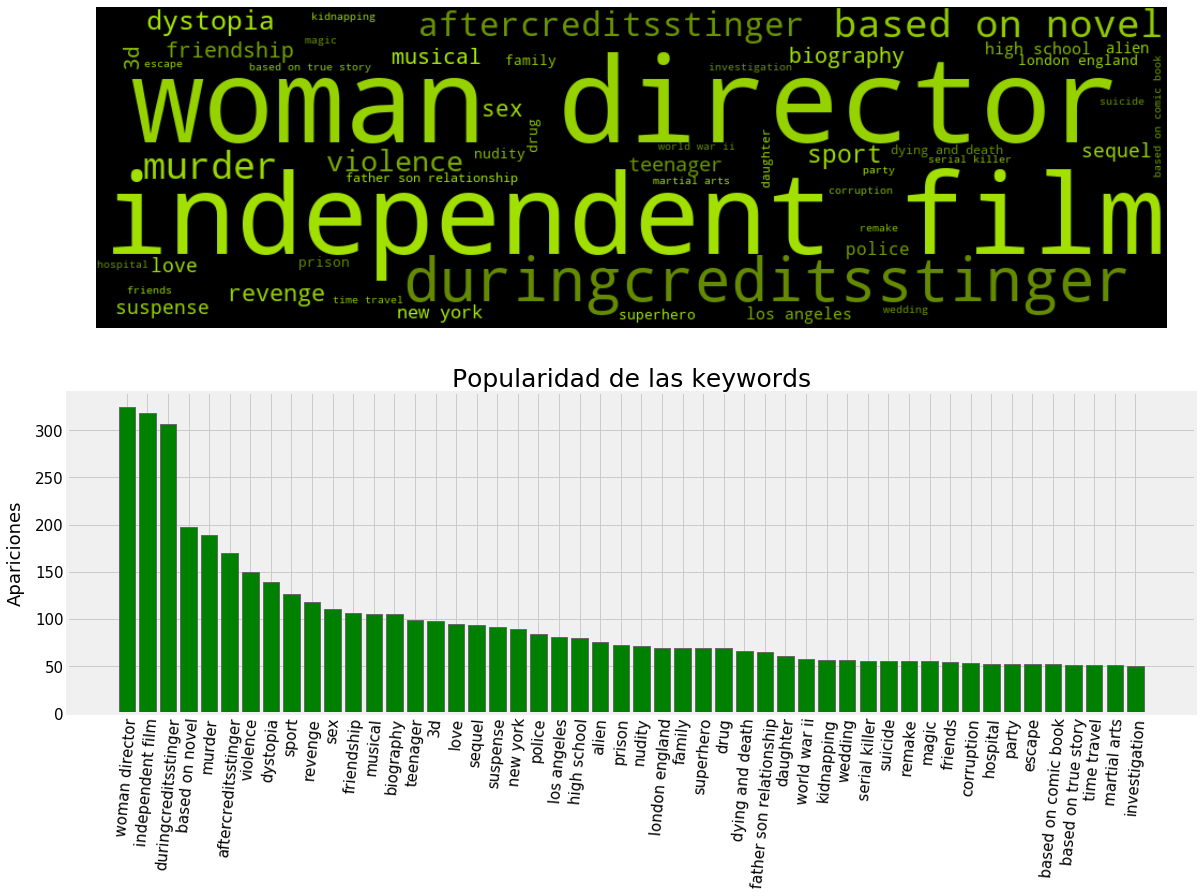
\includegraphics[height=10cm]{./contenido/imagenes/output_17_0.png}
\end{figure}
    { \hspace*{\fill} \\}
    
    \begin{center}\rule{0.5\linewidth}{\linethickness}\end{center}

\subsubsection{1.2 Factor de completitud: Valores
Faltantes}\label{factor-de-completitud-valores-faltantes}

El conjunto de datos consiste en 5043 películas o series que están
descritas mediante 28 variables. Como en todo análisis, habrá que trater
con los valores faltantes y, como un primer paso, se calcula la cantidad
de datos faltantes en cada variable:

    \begin{tcolorbox}[breakable, size=fbox, boxrule=1pt, pad at break*=1mm,colback=cellbackground, colframe=cellborder]
\prompt{In}{incolor}{12}{\hspace{4pt}}
\begin{Verbatim}[commandchars=\\\{\}]
\PY{n}{missing\PYZus{}df} \PY{o}{=} \PY{n}{df\PYZus{}initial}\PY{o}{.}\PY{n}{isnull}\PY{p}{(}\PY{p}{)}\PY{o}{.}\PY{n}{sum}\PY{p}{(}\PY{n}{axis}\PY{o}{=}\PY{l+m+mi}{0}\PY{p}{)}\PY{o}{.}\PY{n}{reset\PYZus{}index}\PY{p}{(}\PY{p}{)}
\PY{n}{missing\PYZus{}df}\PY{o}{.}\PY{n}{columns} \PY{o}{=} \PY{p}{[}\PY{l+s+s1}{\PYZsq{}}\PY{l+s+s1}{column\PYZus{}name}\PY{l+s+s1}{\PYZsq{}}\PY{p}{,} \PY{l+s+s1}{\PYZsq{}}\PY{l+s+s1}{missing\PYZus{}count}\PY{l+s+s1}{\PYZsq{}}\PY{p}{]}
\PY{n}{missing\PYZus{}df}\PY{p}{[}\PY{l+s+s1}{\PYZsq{}}\PY{l+s+s1}{filling\PYZus{}factor}\PY{l+s+s1}{\PYZsq{}}\PY{p}{]} \PY{o}{=} \PY{p}{(}\PY{n}{df\PYZus{}initial}\PY{o}{.}\PY{n}{shape}\PY{p}{[}\PY{l+m+mi}{0}\PY{p}{]} 
                                \PY{o}{\PYZhy{}} \PY{n}{missing\PYZus{}df}\PY{p}{[}\PY{l+s+s1}{\PYZsq{}}\PY{l+s+s1}{missing\PYZus{}count}\PY{l+s+s1}{\PYZsq{}}\PY{p}{]}\PY{p}{)} \PY{o}{/} \PY{n}{df\PYZus{}initial}\PY{o}{.}\PY{n}{shape}\PY{p}{[}\PY{l+m+mi}{0}\PY{p}{]} \PY{o}{*} \PY{l+m+mi}{100}
\PY{n}{missing\PYZus{}df}\PY{o}{.}\PY{n}{sort\PYZus{}values}\PY{p}{(}\PY{l+s+s1}{\PYZsq{}}\PY{l+s+s1}{filling\PYZus{}factor}\PY{l+s+s1}{\PYZsq{}}\PY{p}{)}\PY{o}{.}\PY{n}{reset\PYZus{}index}\PY{p}{(}\PY{n}{drop} \PY{o}{=} \PY{k+kc}{True}\PY{p}{)}
\end{Verbatim}
\end{tcolorbox}

            \begin{tcolorbox}[breakable, boxrule=.5pt, size=fbox, pad at break*=1mm, opacityfill=0]
\prompt{Out}{outcolor}{12}{\hspace{3.5pt}}
\begin{Verbatim}[commandchars=\\\{\}]
             column\_name  missing\_count  filling\_factor
0               homepage           3091       35.644389
1                tagline            844       82.427649
2                country            174       96.377264
3           actor\_3\_name             93       98.063710
4               language             86       98.209452
5           actor\_2\_name             63       98.688320
6           actor\_1\_name             53       98.896523
7          director\_name             30       99.375390
8               overview              3       99.937539
9               duration              2       99.958359
10            title\_year              1       99.979180
11          release\_date              1       99.979180
12       num\_voted\_users              0      100.000000
13          vote\_average              0      100.000000
14           movie\_title              0      100.000000
15                budget              0      100.000000
16      spoken\_languages              0      100.000000
17  production\_countries              0      100.000000
18  production\_companies              0      100.000000
19            popularity              0      100.000000
20        original\_title              0      100.000000
21         plot\_keywords              0      100.000000
22                    id              0      100.000000
23                genres              0      100.000000
24                status              0      100.000000
25                 gross              0      100.000000
\end{Verbatim}
\end{tcolorbox}
        
    Podemos ver que la integridad de los datos es bastante buena, ya que
únicamente 2 de las 28 variables tienen un factor de competitud menor
del 93\%.

    \begin{center}\rule{0.5\linewidth}{\linethickness}\end{center}

\subsubsection{~1.3 Películas por año}\label{peluxedculas-por-auxf1o}

    La variable \textbf{title\_year} indica cuándo se lanzó una película.
Para tener una visión global de la forma en la que las películas se
distribuyen según esta variable, las agrupamos por décadas:

    \begin{tcolorbox}[breakable, size=fbox, boxrule=1pt, pad at break*=1mm,colback=cellbackground, colframe=cellborder]
\prompt{In}{incolor}{13}{\hspace{4pt}}
\begin{Verbatim}[commandchars=\\\{\}]
\PY{c+c1}{\PYZsh{}Obtenemos la década de cada película}

\PY{n}{df\PYZus{}initial}\PY{p}{[}\PY{l+s+s1}{\PYZsq{}}\PY{l+s+s1}{decade}\PY{l+s+s1}{\PYZsq{}}\PY{p}{]} \PY{o}{=} \PY{n}{df\PYZus{}initial}\PY{p}{[}\PY{l+s+s1}{\PYZsq{}}\PY{l+s+s1}{title\PYZus{}year}\PY{l+s+s1}{\PYZsq{}}\PY{p}{]}\PY{o}{.}\PY{n}{apply}\PY{p}{(}\PY{k}{lambda} \PY{n}{x}\PY{p}{:}\PY{p}{(}\PY{p}{(}\PY{n}{x}\PY{o}{\PYZhy{}}\PY{l+m+mi}{1900}\PY{p}{)}\PY{o}{/}\PY{o}{/}\PY{l+m+mi}{10}\PY{p}{)}\PY{o}{*}\PY{l+m+mi}{10}\PY{p}{)}
\PY{k}{def} \PY{n+nf}{get\PYZus{}stats}\PY{p}{(}\PY{n}{gr}\PY{p}{)}\PY{p}{:}
    \PY{l+s+sd}{\PYZdq{}\PYZdq{}\PYZdq{}Devuelve las estadísticas de un DataFrame agrupado}
\PY{l+s+sd}{    }
\PY{l+s+sd}{    Arguments:}
\PY{l+s+sd}{        gr \PYZhy{}\PYZhy{} DataFrame agrupado}
\PY{l+s+sd}{    }
\PY{l+s+sd}{    Returns:}
\PY{l+s+sd}{        dict \PYZhy{}\PYZhy{} Diccionario que contiene las estadísticas principales de cada grupo}
\PY{l+s+sd}{    \PYZdq{}\PYZdq{}\PYZdq{}}
    \PY{k}{return} \PY{p}{\PYZob{}}\PY{l+s+s1}{\PYZsq{}}\PY{l+s+s1}{min}\PY{l+s+s1}{\PYZsq{}}\PY{p}{:}\PY{n}{gr}\PY{o}{.}\PY{n}{min}\PY{p}{(}\PY{p}{)}\PY{p}{,}\PY{l+s+s1}{\PYZsq{}}\PY{l+s+s1}{max}\PY{l+s+s1}{\PYZsq{}}\PY{p}{:}\PY{n}{gr}\PY{o}{.}\PY{n}{max}\PY{p}{(}\PY{p}{)}\PY{p}{,}\PY{l+s+s1}{\PYZsq{}}\PY{l+s+s1}{count}\PY{l+s+s1}{\PYZsq{}}\PY{p}{:} \PY{n}{gr}\PY{o}{.}\PY{n}{count}\PY{p}{(}\PY{p}{)}\PY{p}{,}\PY{l+s+s1}{\PYZsq{}}\PY{l+s+s1}{mean}\PY{l+s+s1}{\PYZsq{}}\PY{p}{:}\PY{n}{gr}\PY{o}{.}\PY{n}{mean}\PY{p}{(}\PY{p}{)}\PY{p}{\PYZcb{}}\PY{c+c1}{\PYZsh{}\PYZus{}\PYZus{}\PYZus{}\PYZus{}\PYZus{}\PYZus{}\PYZus{}\PYZus{}\PYZus{}\PYZus{}\PYZus{}\PYZus{}\PYZus{}\PYZus{}\PYZus{}\PYZus{}\PYZus{}\PYZus{}\PYZus{}\PYZus{}\PYZus{}\PYZus{}\PYZus{}\PYZus{}\PYZus{}\PYZus{}\PYZus{}\PYZus{}\PYZus{}\PYZus{}\PYZus{}\PYZus{}\PYZus{}\PYZus{}\PYZus{}\PYZus{}\PYZus{}\PYZus{}\PYZus{}\PYZus{}\PYZus{}\PYZus{}\PYZus{}\PYZus{}\PYZus{}\PYZus{}\PYZus{}\PYZus{}\PYZus{}\PYZus{}\PYZus{}\PYZus{}\PYZus{}\PYZus{}\PYZus{}\PYZus{}\PYZus{}\PYZus{}\PYZus{}\PYZus{}\PYZus{}\PYZus{}}
\PY{c+c1}{\PYZsh{} Creación de un DataFrame con información estadística de cada década}
\PY{n}{test} \PY{o}{=} \PY{n}{df\PYZus{}initial}\PY{p}{[}\PY{l+s+s1}{\PYZsq{}}\PY{l+s+s1}{title\PYZus{}year}\PY{l+s+s1}{\PYZsq{}}\PY{p}{]}\PY{o}{.}\PY{n}{groupby}\PY{p}{(}\PY{n}{df\PYZus{}initial}\PY{p}{[}\PY{l+s+s1}{\PYZsq{}}\PY{l+s+s1}{decade}\PY{l+s+s1}{\PYZsq{}}\PY{p}{]}\PY{p}{)}\PY{o}{.}\PY{n}{apply}\PY{p}{(}\PY{n}{get\PYZus{}stats}\PY{p}{)}\PY{o}{.}\PY{n}{unstack}\PY{p}{(}\PY{p}{)}
\end{Verbatim}
\end{tcolorbox}

    y representamos los resultados en un diagrama de sectores

    \begin{tcolorbox}[breakable, size=fbox, boxrule=1pt, pad at break*=1mm,colback=cellbackground, colframe=cellborder]
\prompt{In}{incolor}{14}{\hspace{4pt}}
\begin{Verbatim}[commandchars=\\\{\}]
\PY{n}{sns}\PY{o}{.}\PY{n}{set\PYZus{}context}\PY{p}{(}\PY{l+s+s2}{\PYZdq{}}\PY{l+s+s2}{poster}\PY{l+s+s2}{\PYZdq{}}\PY{p}{,} \PY{n}{font\PYZus{}scale}\PY{o}{=}\PY{l+m+mf}{0.85}\PY{p}{)}


\PY{k}{def} \PY{n+nf}{label}\PY{p}{(}\PY{n}{s}\PY{p}{)}\PY{p}{:}
    \PY{l+s+sd}{\PYZdq{}\PYZdq{}\PYZdq{}}
\PY{l+s+sd}{    Get de label from the decade. If XX Century\PYZhy{}\PYZgt{} last 2 digits.}
\PY{l+s+sd}{    Else \PYZhy{}\PYZgt{} complete year}
\PY{l+s+sd}{    \PYZdq{}\PYZdq{}\PYZdq{}}
    \PY{n}{val} \PY{o}{=} \PY{p}{(}\PY{l+m+mi}{1900} \PY{o}{+} \PY{n}{s}\PY{p}{,} \PY{n}{s}\PY{p}{)}\PY{p}{[}\PY{n}{s} \PY{o}{\PYZlt{}} \PY{l+m+mi}{100}\PY{p}{]}
    \PY{n}{chaine} \PY{o}{=} \PY{l+s+s1}{\PYZsq{}}\PY{l+s+s1}{\PYZsq{}} \PY{k}{if} \PY{n}{s} \PY{o}{\PYZlt{}} \PY{l+m+mi}{50} \PY{k}{else} \PY{l+s+s2}{\PYZdq{}}\PY{l+s+si}{\PYZob{}\PYZcb{}}\PY{l+s+s2}{\PYZsq{}}\PY{l+s+s2}{s}\PY{l+s+s2}{\PYZdq{}}\PY{o}{.}\PY{n}{format}\PY{p}{(}\PY{n+nb}{int}\PY{p}{(}\PY{n}{val}\PY{p}{)}\PY{p}{)}
    \PY{k}{return} \PY{n}{chaine}

\PY{n}{plt}\PY{o}{.}\PY{n}{rc}\PY{p}{(}\PY{l+s+s1}{\PYZsq{}}\PY{l+s+s1}{font}\PY{l+s+s1}{\PYZsq{}}\PY{p}{,} \PY{n}{weight}\PY{o}{=}\PY{l+s+s1}{\PYZsq{}}\PY{l+s+s1}{bold}\PY{l+s+s1}{\PYZsq{}}\PY{p}{)}
\PY{n}{f}\PY{p}{,} \PY{n}{ax} \PY{o}{=} \PY{n}{plt}\PY{o}{.}\PY{n}{subplots}\PY{p}{(}\PY{n}{figsize}\PY{o}{=}\PY{p}{(}\PY{l+m+mi}{11}\PY{p}{,} \PY{l+m+mi}{6}\PY{p}{)}\PY{p}{)}
\PY{n}{labels} \PY{o}{=} \PY{p}{[}\PY{n}{label}\PY{p}{(}\PY{n}{s}\PY{p}{)} \PY{k}{for} \PY{n}{s} \PY{o+ow}{in}  \PY{n}{test}\PY{o}{.}\PY{n}{index}\PY{p}{]}
\PY{n}{sizes}  \PY{o}{=} \PY{n}{test}\PY{p}{[}\PY{l+s+s1}{\PYZsq{}}\PY{l+s+s1}{count}\PY{l+s+s1}{\PYZsq{}}\PY{p}{]}\PY{o}{.}\PY{n}{values}
\PY{n}{explode} \PY{o}{=} \PY{p}{[}\PY{l+m+mf}{0.2} \PY{k}{if} \PY{n}{sizes}\PY{p}{[}\PY{n}{i}\PY{p}{]} \PY{o}{\PYZlt{}} \PY{l+m+mi}{100} \PY{k}{else} \PY{l+m+mf}{0.01} \PY{k}{for} \PY{n}{i} \PY{o+ow}{in} \PY{n+nb}{range}\PY{p}{(}\PY{l+m+mi}{11}\PY{p}{)}\PY{p}{]}
\PY{n}{ax}\PY{o}{.}\PY{n}{pie}\PY{p}{(}\PY{n}{sizes}\PY{p}{,} \PY{n}{explode} \PY{o}{=} \PY{n}{explode}\PY{p}{,} \PY{n}{labels}\PY{o}{=}\PY{n}{labels}\PY{p}{,}
       \PY{n}{autopct} \PY{o}{=} \PY{k}{lambda} \PY{n}{x}\PY{p}{:}\PY{l+s+s1}{\PYZsq{}}\PY{l+s+si}{\PYZob{}:1.0f\PYZcb{}}\PY{l+s+s1}{\PYZpc{}}\PY{l+s+s1}{\PYZsq{}}\PY{o}{.}\PY{n}{format}\PY{p}{(}\PY{n}{x}\PY{p}{)} \PY{k}{if} \PY{n}{x} \PY{o}{\PYZgt{}} \PY{l+m+mi}{1} \PY{k}{else} \PY{l+s+s1}{\PYZsq{}}\PY{l+s+s1}{\PYZsq{}}\PY{p}{,}
       \PY{n}{shadow}\PY{o}{=}\PY{k+kc}{False}\PY{p}{,} \PY{n}{startangle}\PY{o}{=}\PY{l+m+mi}{0}\PY{p}{)}
\PY{n}{ax}\PY{o}{.}\PY{n}{axis}\PY{p}{(}\PY{l+s+s1}{\PYZsq{}}\PY{l+s+s1}{equal}\PY{l+s+s1}{\PYZsq{}}\PY{p}{)}
\PY{n}{ax}\PY{o}{.}\PY{n}{set\PYZus{}title}\PY{p}{(}\PY{l+s+s1}{\PYZsq{}}\PY{l+s+si}{\PYZpc{} d}\PY{l+s+s1}{e películas por década}\PY{l+s+s1}{\PYZsq{}}\PY{p}{,} \PY{n}{fontsize}\PY{o}{=}\PY{l+m+mi}{16}\PY{p}{)}\PY{p}{;}
\PY{n}{df\PYZus{}initial}\PY{o}{.}\PY{n}{drop}\PY{p}{(}\PY{l+s+s1}{\PYZsq{}}\PY{l+s+s1}{decade}\PY{l+s+s1}{\PYZsq{}}\PY{p}{,} \PY{n}{axis}\PY{o}{=}\PY{l+m+mi}{1}\PY{p}{,} \PY{n}{inplace} \PY{o}{=} \PY{k+kc}{True}\PY{p}{)}
\end{Verbatim}
\end{tcolorbox}

\begin{figure}[h]
    \centering
    \captionsetup{width=10cm}
    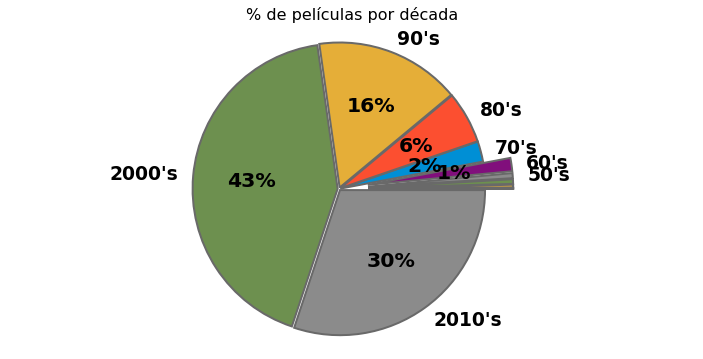
\includegraphics[width=10cm]{./contenido/imagenes/output_25_0.png}

\end{figure}

    { \hspace*{\fill} \\}
    
    \begin{center}\rule{0.5\linewidth}{\linethickness}\end{center}

\subsubsection{1.4 Géneros}\label{guxe9neros}

    La variable \textbf{genres} será importante en la creación del sistema
de recomendación, dado que describe el contenido de la película. Para
ver exactamente qué generos son los mas populares, se usa la misma
aproximación que con las keywords.

    \begin{tcolorbox}[breakable, size=fbox, boxrule=1pt, pad at break*=1mm,colback=cellbackground, colframe=cellborder]
\prompt{In}{incolor}{15}{\hspace{4pt}}
\begin{Verbatim}[commandchars=\\\{\}]
\PY{n}{genre\PYZus{}labels} \PY{o}{=} \PY{n+nb}{set}\PY{p}{(}\PY{p}{)}
\PY{k}{for} \PY{n}{s} \PY{o+ow}{in} \PY{n}{df\PYZus{}initial}\PY{p}{[}\PY{l+s+s1}{\PYZsq{}}\PY{l+s+s1}{genres}\PY{l+s+s1}{\PYZsq{}}\PY{p}{]}\PY{o}{.}\PY{n}{str}\PY{o}{.}\PY{n}{split}\PY{p}{(}\PY{l+s+s1}{\PYZsq{}}\PY{l+s+s1}{|}\PY{l+s+s1}{\PYZsq{}}\PY{p}{)}\PY{o}{.}\PY{n}{values}\PY{p}{:}
    \PY{n}{genre\PYZus{}labels} \PY{o}{=} \PY{n}{genre\PYZus{}labels}\PY{o}{.}\PY{n}{union}\PY{p}{(}\PY{n+nb}{set}\PY{p}{(}\PY{n}{s}\PY{p}{)}\PY{p}{)}
\end{Verbatim}
\end{tcolorbox}

    y cada genero aparece las siguientes veces:

    \begin{tcolorbox}[breakable, size=fbox, boxrule=1pt, pad at break*=1mm,colback=cellbackground, colframe=cellborder]
\prompt{In}{incolor}{16}{\hspace{4pt}}
\begin{Verbatim}[commandchars=\\\{\}]
\PY{n}{keyword\PYZus{}occurences}\PY{p}{,} \PY{n}{dum} \PY{o}{=} \PY{n}{count\PYZus{}word}\PY{p}{(}\PY{n}{df\PYZus{}initial}\PY{p}{,} \PY{l+s+s1}{\PYZsq{}}\PY{l+s+s1}{genres}\PY{l+s+s1}{\PYZsq{}}\PY{p}{,} \PY{n}{genre\PYZus{}labels}\PY{p}{)}
\PY{n}{keyword\PYZus{}occurences}\PY{p}{[}\PY{p}{:}\PY{l+m+mi}{5}\PY{p}{]}
\end{Verbatim}
\end{tcolorbox}

            \begin{tcolorbox}[breakable, boxrule=.5pt, size=fbox, pad at break*=1mm, opacityfill=0]
\prompt{Out}{outcolor}{16}{\hspace{3.5pt}}
\begin{Verbatim}[commandchars=\\\{\}]
[['Drama', 2297],
 ['Comedy', 1722],
 ['Thriller', 1274],
 ['Action', 1154],
 ['Romance', 894]]
\end{Verbatim}
\end{tcolorbox}
        
    \begin{tcolorbox}[breakable, size=fbox, boxrule=1pt, pad at break*=1mm,colback=cellbackground, colframe=cellborder]
\prompt{In}{incolor}{17}{\hspace{4pt}}
\begin{Verbatim}[commandchars=\\\{\}]
\PY{n}{keyword\PYZus{}occurences} \PY{o}{=} \PY{p}{[}\PY{n}{x} \PY{k}{for} \PY{n}{x} \PY{o+ow}{in} \PY{n}{keyword\PYZus{}occurences} \PY{k}{if} \PY{n}{x}\PY{p}{[}\PY{l+m+mi}{0}\PY{p}{]}\PY{p}{]}
\end{Verbatim}
\end{tcolorbox}

    Se muestra el resultado como una nube de palabras

    \begin{tcolorbox}[breakable, size=fbox, boxrule=1pt, pad at break*=1mm,colback=cellbackground, colframe=cellborder]
\prompt{In}{incolor}{18}{\hspace{4pt}}
\begin{Verbatim}[commandchars=\\\{\}]
\PY{n}{words} \PY{o}{=} \PY{n+nb}{dict}\PY{p}{(}\PY{p}{)}
\PY{n}{trunc\PYZus{}occurences} \PY{o}{=} \PY{n}{keyword\PYZus{}occurences}\PY{p}{[}\PY{l+m+mi}{0}\PY{p}{:}\PY{l+m+mi}{50}\PY{p}{]}
\PY{k}{for} \PY{n}{s} \PY{o+ow}{in} \PY{n}{trunc\PYZus{}occurences}\PY{p}{:}
    \PY{n}{words}\PY{p}{[}\PY{n}{s}\PY{p}{[}\PY{l+m+mi}{0}\PY{p}{]}\PY{p}{]} \PY{o}{=} \PY{n}{s}\PY{p}{[}\PY{l+m+mi}{1}\PY{p}{]}
\PY{n}{tone} \PY{o}{=} \PY{l+m+mi}{100} \PY{c+c1}{\PYZsh{} define the color of the words}
\PY{n}{f}\PY{p}{,} \PY{n}{ax} \PY{o}{=} \PY{n}{plt}\PY{o}{.}\PY{n}{subplots}\PY{p}{(}\PY{n}{figsize}\PY{o}{=}\PY{p}{(}\PY{l+m+mi}{14}\PY{p}{,} \PY{l+m+mi}{6}\PY{p}{)}\PY{p}{)}
\PY{n}{wordcloud} \PY{o}{=} \PY{n}{WordCloud}\PY{p}{(}\PY{n}{width}\PY{o}{=}\PY{l+m+mi}{550}\PY{p}{,}\PY{n}{height}\PY{o}{=}\PY{l+m+mi}{300}\PY{p}{,} \PY{n}{background\PYZus{}color}\PY{o}{=}\PY{l+s+s1}{\PYZsq{}}\PY{l+s+s1}{black}\PY{l+s+s1}{\PYZsq{}}\PY{p}{,} 
                      \PY{n}{max\PYZus{}words}\PY{o}{=}\PY{l+m+mi}{1628}\PY{p}{,}\PY{n}{relative\PYZus{}scaling}\PY{o}{=}\PY{l+m+mf}{0.7}\PY{p}{,}
                      \PY{n}{color\PYZus{}func} \PY{o}{=} \PY{n}{random\PYZus{}color\PYZus{}func}\PY{p}{,}
                      \PY{n}{normalize\PYZus{}plurals}\PY{o}{=}\PY{k+kc}{False}\PY{p}{)}
\PY{n}{wordcloud}\PY{o}{.}\PY{n}{generate\PYZus{}from\PYZus{}frequencies}\PY{p}{(}\PY{n}{words}\PY{p}{)}
\PY{n}{plt}\PY{o}{.}\PY{n}{imshow}\PY{p}{(}\PY{n}{wordcloud}\PY{p}{,} \PY{n}{interpolation}\PY{o}{=}\PY{l+s+s2}{\PYZdq{}}\PY{l+s+s2}{bilinear}\PY{l+s+s2}{\PYZdq{}}\PY{p}{)}
\PY{n}{plt}\PY{o}{.}\PY{n}{axis}\PY{p}{(}\PY{l+s+s1}{\PYZsq{}}\PY{l+s+s1}{off}\PY{l+s+s1}{\PYZsq{}}\PY{p}{)}
\PY{n}{plt}\PY{o}{.}\PY{n}{show}\PY{p}{(}\PY{p}{)}
\end{Verbatim}
\end{tcolorbox}
\begin{figure}[h]
    \centering
    \captionsetup{width=10cm}
    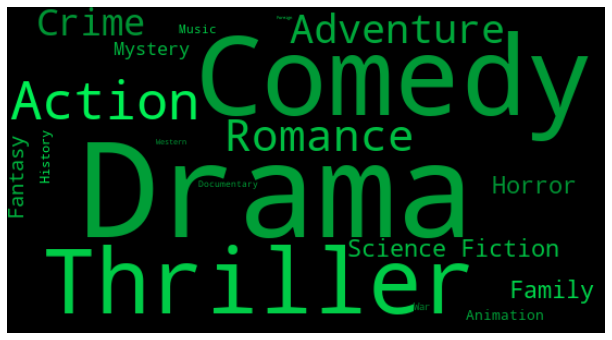
\includegraphics[width=10cm]{./contenido/imagenes/output_33_0.png}
\end{figure}

    { \hspace*{\fill} \\}
    
    \begin{center}\rule{0.5\linewidth}{\linethickness}\end{center}

\subsection{2. Limpieza}\label{limpieza}

\begin{center}\rule{0.5\linewidth}{\linethickness}\end{center}

\subsubsection{2.1 Entradas duplicadas}\label{entradas-duplicadas}

Hasta ahora, sólo mirabamos unas pocas variables e intentábamos
representar su contenido para tener una idea de su significado. Por
tanto, es ahora cuando empieza realmente la tarea de limpieza.

El primer paso consiste en buscar entradas duplicadas. Como un primer
paso, se comprueba si si las hay.

    \begin{tcolorbox}[breakable, size=fbox, boxrule=1pt, pad at break*=1mm,colback=cellbackground, colframe=cellborder]
\prompt{In}{incolor}{19}{\hspace{4pt}}
\begin{Verbatim}[commandchars=\\\{\}]
\PY{n}{doubled\PYZus{}entries} \PY{o}{=} \PY{n}{df\PYZus{}initial}\PY{p}{[}\PY{n}{df\PYZus{}initial}\PY{o}{.}\PY{n}{id}\PY{o}{.}\PY{n}{duplicated}\PY{p}{(}\PY{p}{)}\PY{p}{]}
\PY{n}{doubled\PYZus{}entries}\PY{o}{.}\PY{n}{shape}
\end{Verbatim}
\end{tcolorbox}

            \begin{tcolorbox}[breakable, boxrule=.5pt, size=fbox, pad at break*=1mm, opacityfill=0]
\prompt{Out}{outcolor}{19}{\hspace{3.5pt}}
\begin{Verbatim}[commandchars=\\\{\}]
(0, 26)
\end{Verbatim}
\end{tcolorbox}
        
    \begin{tcolorbox}[breakable, size=fbox, boxrule=1pt, pad at break*=1mm,colback=cellbackground, colframe=cellborder]
\prompt{In}{incolor}{20}{\hspace{4pt}}
\begin{Verbatim}[commandchars=\\\{\}]
\PY{n}{df\PYZus{}temp} \PY{o}{=} \PY{n}{df\PYZus{}initial}
\end{Verbatim}
\end{tcolorbox}

    Ahora examinamos lasfilas con entradas duplicadas teniendo en cuenta
únicamente las variables \textbf{movie\_title} y \textbf{title\_year},
and \textbf{director\_name}:

    \begin{tcolorbox}[breakable, size=fbox, boxrule=1pt, pad at break*=1mm,colback=cellbackground, colframe=cellborder]
\prompt{In}{incolor}{21}{\hspace{4pt}}
\begin{Verbatim}[commandchars=\\\{\}]
\PY{n}{list\PYZus{}var\PYZus{}duplicates} \PY{o}{=} \PY{p}{[}\PY{l+s+s1}{\PYZsq{}}\PY{l+s+s1}{movie\PYZus{}title}\PY{l+s+s1}{\PYZsq{}}\PY{p}{,} \PY{l+s+s1}{\PYZsq{}}\PY{l+s+s1}{title\PYZus{}year}\PY{l+s+s1}{\PYZsq{}}\PY{p}{,} \PY{l+s+s1}{\PYZsq{}}\PY{l+s+s1}{director\PYZus{}name}\PY{l+s+s1}{\PYZsq{}}\PY{p}{]}
\end{Verbatim}
\end{tcolorbox}

    Creamos una lista con las entradas con títulos idénticos:

    \begin{tcolorbox}[breakable, size=fbox, boxrule=1pt, pad at break*=1mm,colback=cellbackground, colframe=cellborder]
\prompt{In}{incolor}{22}{\hspace{4pt}}
\begin{Verbatim}[commandchars=\\\{\}]
\PY{n}{liste\PYZus{}duplicates} \PY{o}{=} \PY{n}{df\PYZus{}temp}\PY{p}{[}\PY{l+s+s1}{\PYZsq{}}\PY{l+s+s1}{movie\PYZus{}title}\PY{l+s+s1}{\PYZsq{}}\PY{p}{]}\PY{o}{.}\PY{n}{map}\PY{p}{(}\PY{n}{df\PYZus{}temp}\PY{p}{[}\PY{l+s+s1}{\PYZsq{}}\PY{l+s+s1}{movie\PYZus{}title}\PY{l+s+s1}{\PYZsq{}}\PY{p}{]}\PY{o}{.}\PY{n}{value\PYZus{}counts}\PY{p}{(}\PY{p}{)} \PY{o}{\PYZgt{}} \PY{l+m+mi}{1}\PY{p}{)}
\PY{n+nb}{print}\PY{p}{(}\PY{l+s+s2}{\PYZdq{}}\PY{l+s+s2}{Número de entradas duplicadas: }\PY{l+s+si}{\PYZob{}\PYZcb{}}\PY{l+s+s2}{\PYZdq{}}\PY{o}{.}\PY{n}{format}\PY{p}{(}
    \PY{n+nb}{len}\PY{p}{(}\PY{n}{df\PYZus{}temp}\PY{p}{[}\PY{n}{liste\PYZus{}duplicates}\PY{p}{]}\PY{p}{[}\PY{n}{list\PYZus{}var\PYZus{}duplicates}\PY{p}{]}\PY{p}{)}\PY{p}{)}\PY{p}{)}
\end{Verbatim}
\end{tcolorbox}

    \begin{Verbatim}[commandchars=\\\{\}]
Número de entradas duplicadas: 6
\end{Verbatim}

    y a continuación examinamos algunos casos. Dado que no hay demasiados
valores, es posible hacerlo a simple vista:

    \begin{tcolorbox}[breakable, size=fbox, boxrule=1pt, pad at break*=1mm,colback=cellbackground, colframe=cellborder]
\prompt{In}{incolor}{23}{\hspace{4pt}}
\begin{Verbatim}[commandchars=\\\{\}]
\PY{n}{df\PYZus{}temp}\PY{p}{[}\PY{n}{liste\PYZus{}duplicates}\PY{p}{]}\PY{p}{[}\PY{n}{list\PYZus{}var\PYZus{}duplicates}\PY{p}{]}\PY{o}{.}\PY{n}{sort\PYZus{}values}\PY{p}{(}\PY{l+s+s1}{\PYZsq{}}\PY{l+s+s1}{movie\PYZus{}title}\PY{l+s+s1}{\PYZsq{}}\PY{p}{)}
\end{Verbatim}
\end{tcolorbox}

            \begin{tcolorbox}[breakable, boxrule=.5pt, size=fbox, pad at break*=1mm, opacityfill=0]
\prompt{Out}{outcolor}{23}{\hspace{3.5pt}}
\begin{Verbatim}[commandchars=\\\{\}]
          movie\_title  title\_year        director\_name
1359           Batman      1989.0           Tim Burton
4267           Batman      1966.0  Leslie H. Martinson
3647  Out of the Blue      1980.0        Dennis Hopper
3693  Out of the Blue      2006.0       Robert Sarkies
972          The Host      2013.0        Andrew Niccol
2877         The Host      2006.0         Bong Joon-ho
\end{Verbatim}
\end{tcolorbox}
        
    Puede verse que estas películas son únicamente remakes.

    \begin{tcolorbox}[breakable, size=fbox, boxrule=1pt, pad at break*=1mm,colback=cellbackground, colframe=cellborder]
\prompt{In}{incolor}{24}{\hspace{4pt}}
\begin{Verbatim}[commandchars=\\\{\}]
\PY{n}{df\PYZus{}duplicate\PYZus{}cleaned} \PY{o}{=} \PY{n}{df\PYZus{}temp}
\end{Verbatim}
\end{tcolorbox}

    \begin{center}\rule{0.5\linewidth}{\linethickness}\end{center}

\subsubsection{2.2 Limpieza de keywords}\label{limpieza-de-keywords}

Las keywords tendrán un papel fundamental en el funcionamiento del
sistema. De hecho, las recomendaciones se basaran en la similaridad
entre películas. Para medir esas similaridades, se mirarán las películas
descritas por las mismas keywords. Por tanto, el contenido de la
variable \textbf{plot\_keywords} debe ser analizado, ya que será muy
utilizado.

    \begin{center}\rule{0.5\linewidth}{\linethickness}\end{center}

\paragraph{2.2.1 Agrupamiento por lexema}\label{agrupamiento-por-lexema}

Cogemos las keywords que aparecen en \textbf{plot\_keywords}. Esta lista
se limpia usando NLTK. Finalmente, veremos la ocurrencia de cada
keyword.

    \begin{tcolorbox}[breakable, size=fbox, boxrule=1pt, pad at break*=1mm,colback=cellbackground, colframe=cellborder]
\prompt{In}{incolor}{25}{\hspace{4pt}}
\begin{Verbatim}[commandchars=\\\{\}]
\PY{k}{def} \PY{n+nf}{keywords\PYZus{}inventory}\PY{p}{(}\PY{n}{dataframe}\PY{p}{,} \PY{n}{column} \PY{o}{=} \PY{l+s+s1}{\PYZsq{}}\PY{l+s+s1}{plot\PYZus{}keywords}\PY{l+s+s1}{\PYZsq{}}\PY{p}{)}\PY{p}{:}
    \PY{l+s+sd}{\PYZdq{}\PYZdq{}\PYZdq{}Devuelve un diccionario con las palabras que derivan de cada lexema}
\PY{l+s+sd}{    a partir de un DataFrame y la columna de la que se quiere extraer}
\PY{l+s+sd}{    }
\PY{l+s+sd}{    Arguments:}
\PY{l+s+sd}{        dataframe \PYZhy{}\PYZhy{} DataFrame del que obtener la información}
\PY{l+s+sd}{    }
\PY{l+s+sd}{    Keyword Arguments:}
\PY{l+s+sd}{        column \PYZob{}str\PYZcb{} \PYZhy{}\PYZhy{} Nombre de la columna (default: \PYZob{}\PYZsq{}plot\PYZus{}keywords\PYZsq{}\PYZcb{})}
\PY{l+s+sd}{    }
\PY{l+s+sd}{    Returns:}
\PY{l+s+sd}{        Lista con las keywords finales que aparecen}
\PY{l+s+sd}{        Diccionario con la relación lexema \PYZlt{}\PYZhy{}\PYZgt{} palabras}
\PY{l+s+sd}{        Diccionario con la palabra más corta derivada del lexema}
\PY{l+s+sd}{    \PYZdq{}\PYZdq{}\PYZdq{}}
    \PY{n}{PS} \PY{o}{=} \PY{n}{nltk}\PY{o}{.}\PY{n}{stem}\PY{o}{.}\PY{n}{PorterStemmer}\PY{p}{(}\PY{p}{)}
    \PY{n}{keywords\PYZus{}roots}  \PY{o}{=} \PY{n+nb}{dict}\PY{p}{(}\PY{p}{)}  \PY{c+c1}{\PYZsh{} recoger las palabras de cada lexema}
    \PY{n}{keywords\PYZus{}select} \PY{o}{=} \PY{n+nb}{dict}\PY{p}{(}\PY{p}{)}  \PY{c+c1}{\PYZsh{} asociacion: lexema \PYZlt{}\PYZhy{}\PYZgt{} keyword}
    \PY{n}{category\PYZus{}keys} \PY{o}{=} \PY{p}{[}\PY{p}{]}
    \PY{n}{icount} \PY{o}{=} \PY{l+m+mi}{0}
    \PY{k}{for} \PY{n}{s} \PY{o+ow}{in} \PY{n}{dataframe}\PY{p}{[}\PY{n}{column}\PY{p}{]}\PY{p}{:}
        \PY{k}{if} \PY{n}{pd}\PY{o}{.}\PY{n}{isnull}\PY{p}{(}\PY{n}{s}\PY{p}{)}\PY{p}{:} \PY{k}{continue}
        \PY{k}{for} \PY{n}{t} \PY{o+ow}{in} \PY{n}{s}\PY{o}{.}\PY{n}{split}\PY{p}{(}\PY{l+s+s1}{\PYZsq{}}\PY{l+s+s1}{|}\PY{l+s+s1}{\PYZsq{}}\PY{p}{)}\PY{p}{:}
            \PY{n}{t} \PY{o}{=} \PY{n}{t}\PY{o}{.}\PY{n}{lower}\PY{p}{(}\PY{p}{)} \PY{p}{;} \PY{n}{root} \PY{o}{=} \PY{n}{PS}\PY{o}{.}\PY{n}{stem}\PY{p}{(}\PY{n}{t}\PY{p}{)}
            \PY{c+c1}{\PYZsh{} Para cada lexema, un set con las palabras que lo usan}
            \PY{k}{if} \PY{n}{root} \PY{o+ow}{in} \PY{n}{keywords\PYZus{}roots}\PY{p}{:}                
                \PY{n}{keywords\PYZus{}roots}\PY{p}{[}\PY{n}{root}\PY{p}{]}\PY{o}{.}\PY{n}{add}\PY{p}{(}\PY{n}{t}\PY{p}{)}
            \PY{k}{else}\PY{p}{:}
                \PY{n}{keywords\PYZus{}roots}\PY{p}{[}\PY{n}{root}\PY{p}{]} \PY{o}{=} \PY{p}{\PYZob{}}\PY{n}{t}\PY{p}{\PYZcb{}}
    
    \PY{k}{for} \PY{n}{s} \PY{o+ow}{in} \PY{n}{keywords\PYZus{}roots}\PY{o}{.}\PY{n}{keys}\PY{p}{(}\PY{p}{)}\PY{p}{:}
        \PY{k}{if} \PY{n+nb}{len}\PY{p}{(}\PY{n}{keywords\PYZus{}roots}\PY{p}{[}\PY{n}{s}\PY{p}{]}\PY{p}{)} \PY{o}{\PYZgt{}} \PY{l+m+mi}{1}\PY{p}{:}  
            \PY{n}{min\PYZus{}length} \PY{o}{=} \PY{l+m+mi}{1000}
            \PY{k}{for} \PY{n}{k} \PY{o+ow}{in} \PY{n}{keywords\PYZus{}roots}\PY{p}{[}\PY{n}{s}\PY{p}{]}\PY{p}{:}
                \PY{k}{if} \PY{n+nb}{len}\PY{p}{(}\PY{n}{k}\PY{p}{)} \PY{o}{\PYZlt{}} \PY{n}{min\PYZus{}length}\PY{p}{:}
                    \PY{n}{key} \PY{o}{=} \PY{n}{k} \PY{p}{;} \PY{n}{min\PYZus{}length} \PY{o}{=} \PY{n+nb}{len}\PY{p}{(}\PY{n}{k}\PY{p}{)}            
            \PY{n}{category\PYZus{}keys}\PY{o}{.}\PY{n}{append}\PY{p}{(}\PY{n}{key}\PY{p}{)}
            \PY{n}{keywords\PYZus{}select}\PY{p}{[}\PY{n}{s}\PY{p}{]} \PY{o}{=} \PY{n}{key}
        \PY{k}{else}\PY{p}{:}
            \PY{n}{category\PYZus{}keys}\PY{o}{.}\PY{n}{append}\PY{p}{(}\PY{n+nb}{list}\PY{p}{(}\PY{n}{keywords\PYZus{}roots}\PY{p}{[}\PY{n}{s}\PY{p}{]}\PY{p}{)}\PY{p}{[}\PY{l+m+mi}{0}\PY{p}{]}\PY{p}{)}
            \PY{n}{keywords\PYZus{}select}\PY{p}{[}\PY{n}{s}\PY{p}{]} \PY{o}{=} \PY{n+nb}{list}\PY{p}{(}\PY{n}{keywords\PYZus{}roots}\PY{p}{[}\PY{n}{s}\PY{p}{]}\PY{p}{)}\PY{p}{[}\PY{l+m+mi}{0}\PY{p}{]}
                   
    \PY{n+nb}{print}\PY{p}{(}\PY{l+s+s2}{\PYZdq{}}\PY{l+s+s2}{Número de keywords en la variable: }\PY{l+s+s2}{\PYZsq{}}\PY{l+s+si}{\PYZob{}\PYZcb{}}\PY{l+s+s2}{\PYZsq{}}\PY{l+s+s2}{: }\PY{l+s+si}{\PYZob{}\PYZcb{}}\PY{l+s+s2}{\PYZdq{}}\PY{o}{.}\PY{n}{format}\PY{p}{(}\PY{n}{column}\PY{p}{,}\PY{n+nb}{len}\PY{p}{(}\PY{n}{category\PYZus{}keys}\PY{p}{)}\PY{p}{)}\PY{p}{)}
    \PY{k}{return} \PY{n}{category\PYZus{}keys}\PY{p}{,} \PY{n}{keywords\PYZus{}roots}\PY{p}{,} \PY{n}{keywords\PYZus{}select}
\end{Verbatim}
\end{tcolorbox}

    \begin{tcolorbox}[breakable, size=fbox, boxrule=1pt, pad at break*=1mm,colback=cellbackground, colframe=cellborder]
\prompt{In}{incolor}{26}{\hspace{4pt}}
\begin{Verbatim}[commandchars=\\\{\}]
\PY{n}{keywords}\PY{p}{,} \PY{n}{keywords\PYZus{}roots}\PY{p}{,} \PY{n}{keywords\PYZus{}select} \PY{o}{=} \PY{n}{keywords\PYZus{}inventory}\PY{p}{(}\PY{n}{df\PYZus{}duplicate\PYZus{}cleaned}\PY{p}{,}
                                                               \PY{n}{column} \PY{o}{=} \PY{l+s+s1}{\PYZsq{}}\PY{l+s+s1}{plot\PYZus{}keywords}\PY{l+s+s1}{\PYZsq{}}\PY{p}{)}
\end{Verbatim}
\end{tcolorbox}

    \begin{Verbatim}[commandchars=\\\{\}]
Número de keywords en la variable: 'plot\_keywords': 9474
\end{Verbatim}

    \begin{tcolorbox}[breakable, size=fbox, boxrule=1pt, pad at break*=1mm,colback=cellbackground, colframe=cellborder]
\prompt{In}{incolor}{27}{\hspace{4pt}}
\begin{Verbatim}[commandchars=\\\{\}]
\PY{c+c1}{\PYZsh{} Muestra de keywords que aparecen en formas similares}
\PY{c+c1}{\PYZsh{}\PYZhy{}\PYZhy{}\PYZhy{}\PYZhy{}\PYZhy{}\PYZhy{}\PYZhy{}\PYZhy{}\PYZhy{}\PYZhy{}\PYZhy{}\PYZhy{}\PYZhy{}\PYZhy{}\PYZhy{}\PYZhy{}\PYZhy{}\PYZhy{}\PYZhy{}\PYZhy{}\PYZhy{}\PYZhy{}\PYZhy{}\PYZhy{}\PYZhy{}\PYZhy{}\PYZhy{}\PYZhy{}\PYZhy{}\PYZhy{}\PYZhy{}\PYZhy{}\PYZhy{}\PYZhy{}\PYZhy{}\PYZhy{}\PYZhy{}\PYZhy{}\PYZhy{}\PYZhy{}\PYZhy{}\PYZhy{}\PYZhy{}\PYZhy{}\PYZhy{}\PYZhy{}\PYZhy{}\PYZhy{}\PYZhy{}\PYZhy{}\PYZhy{}\PYZhy{}\PYZhy{}\PYZhy{}\PYZhy{}\PYZhy{}\PYZhy{}\PYZhy{}\PYZhy{}\PYZhy{}}
\PY{n}{icount} \PY{o}{=} \PY{l+m+mi}{0}
\PY{k}{for} \PY{n}{s} \PY{o+ow}{in} \PY{n}{keywords\PYZus{}roots}\PY{o}{.}\PY{n}{keys}\PY{p}{(}\PY{p}{)}\PY{p}{:}
    \PY{k}{if} \PY{n+nb}{len}\PY{p}{(}\PY{n}{keywords\PYZus{}roots}\PY{p}{[}\PY{n}{s}\PY{p}{]}\PY{p}{)} \PY{o}{\PYZgt{}} \PY{l+m+mi}{1}\PY{p}{:} 
        \PY{n}{icount} \PY{o}{+}\PY{o}{=} \PY{l+m+mi}{1}
        \PY{k}{if} \PY{n}{icount} \PY{o}{\PYZlt{}} \PY{l+m+mi}{15}\PY{p}{:} \PY{n+nb}{print}\PY{p}{(}\PY{n}{icount}\PY{p}{,} \PY{n}{keywords\PYZus{}roots}\PY{p}{[}\PY{n}{s}\PY{p}{]}\PY{p}{,} \PY{n+nb}{len}\PY{p}{(}\PY{n}{keywords\PYZus{}roots}\PY{p}{[}\PY{n}{s}\PY{p}{]}\PY{p}{)}\PY{p}{)}
\end{Verbatim}
\end{tcolorbox}

    \begin{Verbatim}[commandchars=\\\{\}]
1 \{'alienation', 'alien'\} 2
2 \{'spying', 'spy'\} 2
3 \{'vigilante', 'vigilantism'\} 2
4 \{'terror', 'terrorism'\} 2
5 \{'flooding', 'flood'\} 2
6 \{'spiders', 'spider'\} 2
7 \{'horses', 'horse'\} 2
8 \{'music', 'musical'\} 2
9 \{'anime', 'animation', 'animal'\} 3
10 \{'compass', 'compassion'\} 2
11 \{'train', 'training'\} 2
12 \{'sail', 'sailing'\} 2
13 \{'time travel', 'time traveler'\} 2
14 \{'orcs', 'orc'\} 2
\end{Verbatim}

    \begin{tcolorbox}[breakable, size=fbox, boxrule=1pt, pad at break*=1mm,colback=cellbackground, colframe=cellborder]
\prompt{In}{incolor}{28}{\hspace{4pt}}
\begin{Verbatim}[commandchars=\\\{\}]
\PY{c+c1}{\PYZsh{} Reemplazo de keywords por su forma principal}
\PY{c+c1}{\PYZsh{}\PYZhy{}\PYZhy{}\PYZhy{}\PYZhy{}\PYZhy{}\PYZhy{}\PYZhy{}\PYZhy{}\PYZhy{}\PYZhy{}\PYZhy{}\PYZhy{}\PYZhy{}\PYZhy{}\PYZhy{}\PYZhy{}\PYZhy{}\PYZhy{}\PYZhy{}\PYZhy{}\PYZhy{}\PYZhy{}\PYZhy{}\PYZhy{}\PYZhy{}\PYZhy{}\PYZhy{}\PYZhy{}\PYZhy{}\PYZhy{}\PYZhy{}\PYZhy{}\PYZhy{}\PYZhy{}\PYZhy{}\PYZhy{}\PYZhy{}\PYZhy{}\PYZhy{}\PYZhy{}\PYZhy{}\PYZhy{}\PYZhy{}\PYZhy{}\PYZhy{}\PYZhy{}}
\PY{k}{def} \PY{n+nf}{df\PYZus{}keywords\PYZus{}replacement}\PY{p}{(}\PY{n}{df}\PY{p}{,} \PY{n}{replacement\PYZus{}dict}\PY{p}{,} \PY{n}{roots} \PY{o}{=} \PY{k+kc}{False}\PY{p}{,} \PY{n}{column} \PY{o}{=} \PY{l+s+s1}{\PYZsq{}}\PY{l+s+s1}{plot\PYZus{}keywords}\PY{l+s+s1}{\PYZsq{}}\PY{p}{)}\PY{p}{:}
    \PY{l+s+sd}{\PYZdq{}\PYZdq{}\PYZdq{}Reemplaza las palabras clave de una película por las formas básicas de las mismas.}

\PY{l+s+sd}{    Arguments:}
\PY{l+s+sd}{        df \PYZhy{}\PYZhy{} DataFrame que contiene la información de las películas}
\PY{l+s+sd}{        replacement\PYZus{}dict \PYZhy{}\PYZhy{} diccionarion]}

\PY{l+s+sd}{    Keyword Arguments:}
\PY{l+s+sd}{        roots \PYZob{}bool\PYZcb{} \PYZhy{}\PYZhy{} Controla si se obtienen las raices de las palabras de las}
\PY{l+s+sd}{        keywords (default: \PYZob{}False\PYZcb{})}
\PY{l+s+sd}{        column \PYZhy{}\PYZhy{} Columna en la que realizar la transformación}

\PY{l+s+sd}{    Returns:}
\PY{l+s+sd}{        df\PYZus{}new \PYZhy{}\PYZhy{} DataFrame con las sustituciones realizadas}
\PY{l+s+sd}{    \PYZdq{}\PYZdq{}\PYZdq{}}
    \PY{n}{PS} \PY{o}{=} \PY{n}{nltk}\PY{o}{.}\PY{n}{stem}\PY{o}{.}\PY{n}{PorterStemmer}\PY{p}{(}\PY{p}{)}
    \PY{n}{df\PYZus{}new} \PY{o}{=} \PY{n}{df}\PY{o}{.}\PY{n}{copy}\PY{p}{(}\PY{n}{deep} \PY{o}{=} \PY{k+kc}{True}\PY{p}{)}
    \PY{k}{for} \PY{n}{index}\PY{p}{,} \PY{n}{row} \PY{o+ow}{in} \PY{n}{df\PYZus{}new}\PY{o}{.}\PY{n}{iterrows}\PY{p}{(}\PY{p}{)}\PY{p}{:}
        \PY{n}{chain} \PY{o}{=} \PY{n}{row}\PY{p}{[}\PY{n}{column}\PY{p}{]}
        \PY{k}{if} \PY{n}{pd}\PY{o}{.}\PY{n}{isnull}\PY{p}{(}\PY{n}{chain}\PY{p}{)}\PY{p}{:} \PY{k}{continue}
        \PY{n}{new\PYZus{}list} \PY{o}{=} \PY{p}{[}\PY{p}{]}
        \PY{k}{for} \PY{n}{s} \PY{o+ow}{in} \PY{n}{chain}\PY{o}{.}\PY{n}{split}\PY{p}{(}\PY{l+s+s1}{\PYZsq{}}\PY{l+s+s1}{|}\PY{l+s+s1}{\PYZsq{}}\PY{p}{)}\PY{p}{:} 
            \PY{n}{key} \PY{o}{=} \PY{n}{PS}\PY{o}{.}\PY{n}{stem}\PY{p}{(}\PY{n}{s}\PY{p}{)} \PY{k}{if} \PY{n}{roots} \PY{k}{else} \PY{n}{s}
            \PY{k}{if} \PY{n}{key} \PY{o+ow}{in} \PY{n}{replacement\PYZus{}dict}\PY{o}{.}\PY{n}{keys}\PY{p}{(}\PY{p}{)}\PY{p}{:}
                \PY{n}{new\PYZus{}list}\PY{o}{.}\PY{n}{append}\PY{p}{(}\PY{n}{replacement\PYZus{}dict}\PY{p}{[}\PY{n}{key}\PY{p}{]}\PY{p}{)}
            \PY{k}{else}\PY{p}{:}
                \PY{n}{new\PYZus{}list}\PY{o}{.}\PY{n}{append}\PY{p}{(}\PY{n}{s}\PY{p}{)}       
        \PY{n}{df\PYZus{}new}\PY{o}{.}\PY{n}{set\PYZus{}value}\PY{p}{(}\PY{n}{index}\PY{p}{,} \PY{n}{column}\PY{p}{,} \PY{l+s+s1}{\PYZsq{}}\PY{l+s+s1}{|}\PY{l+s+s1}{\PYZsq{}}\PY{o}{.}\PY{n}{join}\PY{p}{(}\PY{n}{new\PYZus{}list}\PY{p}{)}\PY{p}{)} 
    \PY{k}{return} \PY{n}{df\PYZus{}new}
\end{Verbatim}
\end{tcolorbox}

    \begin{tcolorbox}[breakable, size=fbox, boxrule=1pt, pad at break*=1mm,colback=cellbackground, colframe=cellborder]
\prompt{In}{incolor}{29}{\hspace{4pt}}
\begin{Verbatim}[commandchars=\\\{\}]
\PY{c+c1}{\PYZsh{} Reemplazo de keywords por su forma principal}
\PY{c+c1}{\PYZsh{}\PYZhy{}\PYZhy{}\PYZhy{}\PYZhy{}\PYZhy{}\PYZhy{}\PYZhy{}\PYZhy{}\PYZhy{}\PYZhy{}\PYZhy{}\PYZhy{}\PYZhy{}\PYZhy{}\PYZhy{}\PYZhy{}\PYZhy{}\PYZhy{}\PYZhy{}\PYZhy{}\PYZhy{}\PYZhy{}\PYZhy{}\PYZhy{}\PYZhy{}\PYZhy{}\PYZhy{}\PYZhy{}\PYZhy{}\PYZhy{}\PYZhy{}\PYZhy{}\PYZhy{}\PYZhy{}\PYZhy{}\PYZhy{}\PYZhy{}\PYZhy{}\PYZhy{}\PYZhy{}\PYZhy{}\PYZhy{}\PYZhy{}\PYZhy{}\PYZhy{}\PYZhy{}\PYZhy{}\PYZhy{}\PYZhy{}}
\PY{n}{df\PYZus{}keywords\PYZus{}cleaned} \PY{o}{=} \PY{n}{df\PYZus{}keywords\PYZus{}replacement}\PY{p}{(}\PY{n}{df\PYZus{}duplicate\PYZus{}cleaned}\PY{p}{,} \PY{n}{keywords\PYZus{}select}\PY{p}{,}
                                               \PY{n}{roots} \PY{o}{=} \PY{k+kc}{True}\PY{p}{)}
\end{Verbatim}
\end{tcolorbox}

    \begin{tcolorbox}[breakable, size=fbox, boxrule=1pt, pad at break*=1mm,colback=cellbackground, colframe=cellborder]
\prompt{In}{incolor}{30}{\hspace{4pt}}
\begin{Verbatim}[commandchars=\\\{\}]
\PY{c+c1}{\PYZsh{} Conteo de la repetición de cada Keyword}
\PY{c+c1}{\PYZsh{}\PYZhy{}\PYZhy{}\PYZhy{}\PYZhy{}\PYZhy{}\PYZhy{}\PYZhy{}\PYZhy{}\PYZhy{}\PYZhy{}\PYZhy{}\PYZhy{}\PYZhy{}\PYZhy{}\PYZhy{}\PYZhy{}\PYZhy{}\PYZhy{}\PYZhy{}\PYZhy{}\PYZhy{}\PYZhy{}\PYZhy{}\PYZhy{}\PYZhy{}\PYZhy{}\PYZhy{}\PYZhy{}\PYZhy{}\PYZhy{}\PYZhy{}\PYZhy{}\PYZhy{}\PYZhy{}}
\PY{n}{keyword\PYZus{}occurences}\PY{p}{,} \PY{n}{keywords\PYZus{}count} \PY{o}{=} \PY{n}{count\PYZus{}word}\PY{p}{(}\PY{n}{df\PYZus{}keywords\PYZus{}cleaned}\PY{p}{,}\PY{l+s+s1}{\PYZsq{}}\PY{l+s+s1}{plot\PYZus{}keywords}\PY{l+s+s1}{\PYZsq{}}\PY{p}{,}\PY{n}{keywords}\PY{p}{)}
\PY{n}{keyword\PYZus{}occurences}\PY{p}{[}\PY{p}{:}\PY{l+m+mi}{5}\PY{p}{]}
\end{Verbatim}
\end{tcolorbox}

            \begin{tcolorbox}[breakable, boxrule=.5pt, size=fbox, pad at break*=1mm, opacityfill=0]
\prompt{Out}{outcolor}{30}{\hspace{3.5pt}}
\begin{Verbatim}[commandchars=\\\{\}]
[['', 412],
 ['woman director', 324],
 ['independent film', 318],
 ['duringcreditsstinger', 307],
 ['based on novel', 197]]
\end{Verbatim}
\end{tcolorbox}
        
    \begin{center}\rule{0.5\linewidth}{\linethickness}\end{center}

\paragraph{\texorpdfstring{2.2.2 Grupos de
\emph{sinónimos}}{2.2.2 Grupos de sinónimos}}\label{grupos-de-sinuxf3nimos}

Limpiamos la lista de keywords en dos pasos. En un primer paso, se
suprimer las keywords que aparecen menos de 5 veces y se reemplazan por
un sinónimo de mayor frecuencia. En un segundo paso, se suprimen las
keywords que aparecen en menos de 3 películas.

    \begin{tcolorbox}[breakable, size=fbox, boxrule=1pt, pad at break*=1mm,colback=cellbackground, colframe=cellborder]
\prompt{In}{incolor}{33}{\hspace{4pt}}
\begin{Verbatim}[commandchars=\\\{\}]
\PY{c+c1}{\PYZsh{} Obtener los sinónimos de la palabra \PYZsq{}keyword\PYZsq{}}
\PY{c+c1}{\PYZsh{}\PYZhy{}\PYZhy{}\PYZhy{}\PYZhy{}\PYZhy{}\PYZhy{}\PYZhy{}\PYZhy{}\PYZhy{}\PYZhy{}\PYZhy{}\PYZhy{}\PYZhy{}\PYZhy{}\PYZhy{}\PYZhy{}\PYZhy{}\PYZhy{}\PYZhy{}\PYZhy{}\PYZhy{}\PYZhy{}\PYZhy{}\PYZhy{}\PYZhy{}\PYZhy{}\PYZhy{}\PYZhy{}\PYZhy{}\PYZhy{}\PYZhy{}\PYZhy{}\PYZhy{}\PYZhy{}\PYZhy{}\PYZhy{}\PYZhy{}\PYZhy{}\PYZhy{}\PYZhy{}\PYZhy{}\PYZhy{}\PYZhy{}\PYZhy{}\PYZhy{}\PYZhy{}\PYZhy{}\PYZhy{}\PYZhy{}\PYZhy{}\PYZhy{}\PYZhy{}\PYZhy{}\PYZhy{}\PYZhy{}\PYZhy{}\PYZhy{}\PYZhy{}\PYZhy{}\PYZhy{}\PYZhy{}\PYZhy{}}
\PY{k}{def} \PY{n+nf}{get\PYZus{}synonyms}\PY{p}{(}\PY{n}{keyword}\PY{p}{)}\PY{p}{:}
    \PY{l+s+sd}{\PYZdq{}\PYZdq{}\PYZdq{}Se obtienen los sinónimos sustantivos de una palabra}

\PY{l+s+sd}{    Arguments:}
\PY{l+s+sd}{        keyword \PYZhy{}\PYZhy{} Palabra de la que obtener los sinónimos}


\PY{l+s+sd}{    Returns:}
\PY{l+s+sd}{        lemma \PYZhy{}\PYZhy{} Lista con los sinónimos}
\PY{l+s+sd}{    \PYZdq{}\PYZdq{}\PYZdq{}}

    \PY{n}{lemma} \PY{o}{=} \PY{n+nb}{set}\PY{p}{(}\PY{p}{)}
    \PY{k}{for} \PY{n}{ss} \PY{o+ow}{in} \PY{n}{wordnet}\PY{o}{.}\PY{n}{synsets}\PY{p}{(}\PY{n}{keyword}\PY{p}{)}\PY{p}{:}
        \PY{k}{for} \PY{n}{w} \PY{o+ow}{in} \PY{n}{ss}\PY{o}{.}\PY{n}{lemma\PYZus{}names}\PY{p}{(}\PY{p}{)}\PY{p}{:}
            \PY{c+c1}{\PYZsh{}\PYZus{}\PYZus{}\PYZus{}\PYZus{}\PYZus{}\PYZus{}\PYZus{}\PYZus{}\PYZus{}\PYZus{}\PYZus{}\PYZus{}\PYZus{}\PYZus{}\PYZus{}\PYZus{}\PYZus{}\PYZus{}\PYZus{}\PYZus{}\PYZus{}\PYZus{}\PYZus{}\PYZus{}\PYZus{}\PYZus{}\PYZus{}\PYZus{}\PYZus{}\PYZus{}\PYZus{}}
            \PY{c+c1}{\PYZsh{}  Obtenemos los sinónimos que son sustantivos}
            \PY{n}{index} \PY{o}{=} \PY{n}{ss}\PY{o}{.}\PY{n}{name}\PY{p}{(}\PY{p}{)}\PY{o}{.}\PY{n}{find}\PY{p}{(}\PY{l+s+s1}{\PYZsq{}}\PY{l+s+s1}{.}\PY{l+s+s1}{\PYZsq{}}\PY{p}{)}\PY{o}{+}\PY{l+m+mi}{1}
            \PY{k}{if} \PY{n}{ss}\PY{o}{.}\PY{n}{name}\PY{p}{(}\PY{p}{)}\PY{p}{[}\PY{n}{index}\PY{p}{]} \PY{o}{==} \PY{l+s+s1}{\PYZsq{}}\PY{l+s+s1}{n}\PY{l+s+s1}{\PYZsq{}}\PY{p}{:} \PY{n}{lemma}\PY{o}{.}\PY{n}{add}\PY{p}{(}\PY{n}{w}\PY{o}{.}\PY{n}{lower}\PY{p}{(}\PY{p}{)}\PY{o}{.}\PY{n}{replace}\PY{p}{(}\PY{l+s+s1}{\PYZsq{}}\PY{l+s+s1}{\PYZus{}}\PY{l+s+s1}{\PYZsq{}}\PY{p}{,}\PY{l+s+s1}{\PYZsq{}}\PY{l+s+s1}{ }\PY{l+s+s1}{\PYZsq{}}\PY{p}{)}\PY{p}{)}
    \PY{k}{return} \PY{n}{lemma}   
\end{Verbatim}
\end{tcolorbox}

    \begin{tcolorbox}[breakable, size=fbox, boxrule=1pt, pad at break*=1mm,colback=cellbackground, colframe=cellborder]
\prompt{In}{incolor}{34}{\hspace{4pt}}
\begin{Verbatim}[commandchars=\\\{\}]
\PY{c+c1}{\PYZsh{} Ejemplo de una lista de sinónimos dados por NLTK}
\PY{c+c1}{\PYZsh{}\PYZhy{}\PYZhy{}\PYZhy{}\PYZhy{}\PYZhy{}\PYZhy{}\PYZhy{}\PYZhy{}\PYZhy{}\PYZhy{}\PYZhy{}\PYZhy{}\PYZhy{}\PYZhy{}\PYZhy{}\PYZhy{}\PYZhy{}\PYZhy{}\PYZhy{}\PYZhy{}\PYZhy{}\PYZhy{}\PYZhy{}\PYZhy{}\PYZhy{}\PYZhy{}\PYZhy{}\PYZhy{}\PYZhy{}\PYZhy{}\PYZhy{}\PYZhy{}\PYZhy{}\PYZhy{}\PYZhy{}\PYZhy{}\PYZhy{}\PYZhy{}\PYZhy{}\PYZhy{}\PYZhy{}\PYZhy{}\PYZhy{}\PYZhy{}\PYZhy{}\PYZhy{}\PYZhy{}\PYZhy{}\PYZhy{}\PYZhy{}\PYZhy{}}
\PY{n}{keyword} \PY{o}{=} \PY{l+s+s1}{\PYZsq{}}\PY{l+s+s1}{alien}\PY{l+s+s1}{\PYZsq{}}
\PY{n}{lemma} \PY{o}{=} \PY{n}{get\PYZus{}synonyms}\PY{p}{(}\PY{n}{keyword}\PY{p}{)}
\PY{k}{for} \PY{n}{s} \PY{o+ow}{in} \PY{n}{lemma}\PY{p}{:}
    \PY{n+nb}{print}\PY{p}{(}\PY{l+s+s1}{\PYZsq{}}\PY{l+s+s1}{ }\PY{l+s+s1}{\PYZdq{}}\PY{l+s+si}{\PYZob{}:\PYZlt{}30\PYZcb{}}\PY{l+s+s1}{\PYZdq{}}\PY{l+s+s1}{ in keywords list \PYZhy{}\PYZgt{} }\PY{l+s+si}{\PYZob{}\PYZcb{}}\PY{l+s+s1}{ }\PY{l+s+si}{\PYZob{}\PYZcb{}}\PY{l+s+s1}{\PYZsq{}}\PY{o}{.}\PY{n}{format}\PY{p}{(}\PY{n}{s}\PY{p}{,} \PY{n}{s} \PY{o+ow}{in} \PY{n}{keywords}\PY{p}{,}
                                                \PY{n}{keywords\PYZus{}count}\PY{p}{[}\PY{n}{s}\PY{p}{]} \PY{k}{if} \PY{n}{s} \PY{o+ow}{in} \PY{n}{keywords} \PY{k}{else} \PY{l+m+mi}{0} \PY{p}{)}\PY{p}{)}
\end{Verbatim}
\end{tcolorbox}

    \begin{Verbatim}[commandchars=\\\{\}]
 "extraterrestrial              " in keywords list -> True 4
 "unknown                       " in keywords list -> False 0
 "alien                         " in keywords list -> True 80
 "stranger                      " in keywords list -> True 7
 "extraterrestrial being        " in keywords list -> False 0
 "foreigner                     " in keywords list -> False 0
 "noncitizen                    " in keywords list -> False 0
 "outlander                     " in keywords list -> False 0
\end{Verbatim}

    \begin{tcolorbox}[breakable, size=fbox, boxrule=1pt, pad at break*=1mm,colback=cellbackground, colframe=cellborder]
\prompt{In}{incolor}{35}{\hspace{4pt}}
\begin{Verbatim}[commandchars=\\\{\}]
\PY{c+c1}{\PYZsh{} Comprobar si \PYZsq{}word\PYZsq{} es una clave con más ocurrecncias que el umbral   }
\PY{c+c1}{\PYZsh{}\PYZhy{}\PYZhy{}\PYZhy{}\PYZhy{}\PYZhy{}\PYZhy{}\PYZhy{}\PYZhy{}\PYZhy{}\PYZhy{}\PYZhy{}\PYZhy{}\PYZhy{}\PYZhy{}\PYZhy{}\PYZhy{}\PYZhy{}\PYZhy{}\PYZhy{}\PYZhy{}\PYZhy{}\PYZhy{}\PYZhy{}\PYZhy{}\PYZhy{}\PYZhy{}\PYZhy{}\PYZhy{}\PYZhy{}\PYZhy{}\PYZhy{}\PYZhy{}\PYZhy{}\PYZhy{}\PYZhy{}\PYZhy{}\PYZhy{}\PYZhy{}\PYZhy{}\PYZhy{}\PYZhy{}\PYZhy{}\PYZhy{}\PYZhy{}\PYZhy{}\PYZhy{}\PYZhy{}\PYZhy{}\PYZhy{}\PYZhy{}\PYZhy{}\PYZhy{}\PYZhy{}\PYZhy{}\PYZhy{}\PYZhy{}\PYZhy{}\PYZhy{}\PYZhy{}\PYZhy{}\PYZhy{}\PYZhy{}\PYZhy{}\PYZhy{}\PYZhy{}\PYZhy{}\PYZhy{}\PYZhy{}\PYZhy{}\PYZhy{}\PYZhy{}\PYZhy{}\PYZhy{}\PYZhy{}\PYZhy{}\PYZhy{}\PYZhy{}\PYZhy{}\PYZhy{}\PYZhy{}\PYZhy{}\PYZhy{}}
\PY{k}{def} \PY{n+nf}{test\PYZus{}keyword}\PY{p}{(}\PY{n}{word}\PY{p}{,} \PY{n}{key\PYZus{}count}\PY{p}{,} \PY{n}{threshold}\PY{p}{)}\PY{p}{:}
    \PY{l+s+sd}{\PYZdq{}\PYZdq{}\PYZdq{}Devuelve si una palabra aparece un número mayor de veces que el umbral señalado}

\PY{l+s+sd}{    Arguments:}
\PY{l+s+sd}{        word \PYZhy{}\PYZhy{} Palabra a busvcar}
\PY{l+s+sd}{        key\PYZus{}count \PYZhy{}\PYZhy{} Diccionario con las apariciones de cada keyword}
\PY{l+s+sd}{        threshold \PYZhy{}\PYZhy{} Umbral}

\PY{l+s+sd}{    Returns:}
\PY{l+s+sd}{        bool \PYZhy{}\PYZhy{} True si aparece un número mayor de veces}
\PY{l+s+sd}{    \PYZdq{}\PYZdq{}\PYZdq{}}
    \PY{k}{return} \PY{p}{(}\PY{k+kc}{False} \PY{p}{,} \PY{k+kc}{True}\PY{p}{)}\PY{p}{[}\PY{n}{key\PYZus{}count}\PY{o}{.}\PY{n}{get}\PY{p}{(}\PY{n}{word}\PY{p}{,} \PY{l+m+mi}{0}\PY{p}{)} \PY{o}{\PYZgt{}}\PY{o}{=} \PY{n}{threshold}\PY{p}{]} 
\end{Verbatim}
\end{tcolorbox}

    \begin{tcolorbox}[breakable, size=fbox, boxrule=1pt, pad at break*=1mm,colback=cellbackground, colframe=cellborder]
\prompt{In}{incolor}{37}{\hspace{4pt}}
\begin{Verbatim}[commandchars=\\\{\}]
\PY{n}{keyword\PYZus{}occurences}\PY{o}{.}\PY{n}{sort}\PY{p}{(}\PY{n}{key} \PY{o}{=} \PY{k}{lambda} \PY{n}{x}\PY{p}{:}\PY{n}{x}\PY{p}{[}\PY{l+m+mi}{1}\PY{p}{]}\PY{p}{,} \PY{n}{reverse} \PY{o}{=} \PY{k+kc}{False}\PY{p}{)}
\PY{n}{key\PYZus{}count} \PY{o}{=} \PY{n+nb}{dict}\PY{p}{(}\PY{p}{)}
\PY{k}{for} \PY{n}{s} \PY{o+ow}{in} \PY{n}{keyword\PYZus{}occurences}\PY{p}{:}
    \PY{n}{key\PYZus{}count}\PY{p}{[}\PY{n}{s}\PY{p}{[}\PY{l+m+mi}{0}\PY{p}{]}\PY{p}{]} \PY{o}{=} \PY{n}{s}\PY{p}{[}\PY{l+m+mi}{1}\PY{p}{]}
\PY{c+c1}{\PYZsh{}\PYZus{}\PYZus{}\PYZus{}\PYZus{}\PYZus{}\PYZus{}\PYZus{}\PYZus{}\PYZus{}\PYZus{}\PYZus{}\PYZus{}\PYZus{}\PYZus{}\PYZus{}\PYZus{}\PYZus{}\PYZus{}\PYZus{}\PYZus{}\PYZus{}\PYZus{}\PYZus{}\PYZus{}\PYZus{}\PYZus{}\PYZus{}\PYZus{}\PYZus{}\PYZus{}\PYZus{}\PYZus{}\PYZus{}\PYZus{}\PYZus{}\PYZus{}\PYZus{}\PYZus{}\PYZus{}\PYZus{}\PYZus{}\PYZus{}\PYZus{}\PYZus{}\PYZus{}\PYZus{}\PYZus{}\PYZus{}\PYZus{}\PYZus{}\PYZus{}\PYZus{}\PYZus{}\PYZus{}\PYZus{}\PYZus{}\PYZus{}\PYZus{}\PYZus{}\PYZus{}\PYZus{}\PYZus{}\PYZus{}\PYZus{}\PYZus{}\PYZus{}\PYZus{}\PYZus{}\PYZus{}\PYZus{}\PYZus{}\PYZus{}\PYZus{}\PYZus{}}
\PY{c+c1}{\PYZsh{} Creación de un diccionario para reemplazar keywords por sinónimos de mayor frecuencia}
\PY{n}{remplacement\PYZus{}word} \PY{o}{=} \PY{n+nb}{dict}\PY{p}{(}\PY{p}{)}
\PY{n}{icount} \PY{o}{=} \PY{l+m+mi}{0}
\PY{k}{for} \PY{n}{index}\PY{p}{,} \PY{p}{[}\PY{n}{word}\PY{p}{,} \PY{n}{nb\PYZus{}apparitions}\PY{p}{]} \PY{o+ow}{in} \PY{n+nb}{enumerate}\PY{p}{(}\PY{n}{keyword\PYZus{}occurences}\PY{p}{)}\PY{p}{:}
    \PY{k}{if} \PY{n}{nb\PYZus{}apparitions} \PY{o}{\PYZgt{}} \PY{l+m+mi}{5}\PY{p}{:} \PY{k}{continue}  \PY{c+c1}{\PYZsh{} Sólo las keywords que aparecen menos de 5 veces}
    \PY{n}{lemma} \PY{o}{=} \PY{n}{get\PYZus{}synonyms}\PY{p}{(}\PY{n}{word}\PY{p}{)}
    \PY{k}{if} \PY{n+nb}{len}\PY{p}{(}\PY{n}{lemma}\PY{p}{)} \PY{o}{==} \PY{l+m+mi}{0}\PY{p}{:} \PY{k}{continue}     \PY{c+c1}{\PYZsh{}Caso de plurales}
    \PY{c+c1}{\PYZsh{}\PYZus{}\PYZus{}\PYZus{}\PYZus{}\PYZus{}\PYZus{}\PYZus{}\PYZus{}\PYZus{}\PYZus{}\PYZus{}\PYZus{}\PYZus{}\PYZus{}\PYZus{}\PYZus{}\PYZus{}\PYZus{}\PYZus{}\PYZus{}\PYZus{}\PYZus{}\PYZus{}\PYZus{}\PYZus{}\PYZus{}\PYZus{}\PYZus{}\PYZus{}\PYZus{}\PYZus{}\PYZus{}\PYZus{}\PYZus{}\PYZus{}\PYZus{}\PYZus{}\PYZus{}\PYZus{}\PYZus{}\PYZus{}\PYZus{}\PYZus{}\PYZus{}\PYZus{}\PYZus{}\PYZus{}\PYZus{}\PYZus{}\PYZus{}\PYZus{}\PYZus{}\PYZus{}\PYZus{}\PYZus{}\PYZus{}\PYZus{}\PYZus{}\PYZus{}\PYZus{}\PYZus{}\PYZus{}\PYZus{}\PYZus{}\PYZus{}}
    \PY{n}{word\PYZus{}list} \PY{o}{=} \PY{p}{[}\PY{p}{(}\PY{n}{s}\PY{p}{,} \PY{n}{key\PYZus{}count}\PY{p}{[}\PY{n}{s}\PY{p}{]}\PY{p}{)} \PY{k}{for} \PY{n}{s} \PY{o+ow}{in} \PY{n}{lemma} 
                  \PY{k}{if} \PY{n}{test\PYZus{}keyword}\PY{p}{(}\PY{n}{s}\PY{p}{,} \PY{n}{key\PYZus{}count}\PY{p}{,} \PY{n}{key\PYZus{}count}\PY{p}{[}\PY{n}{word}\PY{p}{]}\PY{p}{)}\PY{p}{]}
    \PY{n}{word\PYZus{}list}\PY{o}{.}\PY{n}{sort}\PY{p}{(}\PY{n}{key} \PY{o}{=} \PY{k}{lambda} \PY{n}{x}\PY{p}{:}\PY{p}{(}\PY{n}{x}\PY{p}{[}\PY{l+m+mi}{1}\PY{p}{]}\PY{p}{,}\PY{n}{x}\PY{p}{[}\PY{l+m+mi}{0}\PY{p}{]}\PY{p}{)}\PY{p}{,} \PY{n}{reverse} \PY{o}{=} \PY{k+kc}{True}\PY{p}{)}    
    \PY{k}{if} \PY{n+nb}{len}\PY{p}{(}\PY{n}{word\PYZus{}list}\PY{p}{)} \PY{o}{\PYZlt{}}\PY{o}{=} \PY{l+m+mi}{1}\PY{p}{:} \PY{k}{continue}       \PY{c+c1}{\PYZsh{} NO se reemplaza}
    \PY{k}{if} \PY{n}{word} \PY{o}{==} \PY{n}{word\PYZus{}list}\PY{p}{[}\PY{l+m+mi}{0}\PY{p}{]}\PY{p}{[}\PY{l+m+mi}{0}\PY{p}{]}\PY{p}{:} \PY{k}{continue}    \PY{c+c1}{\PYZsh{} Reemplazo por sí mismo}
    \PY{n}{icount} \PY{o}{+}\PY{o}{=} \PY{l+m+mi}{1}
    \PY{k}{if}  \PY{n}{icount} \PY{o}{\PYZlt{}} \PY{l+m+mi}{8}\PY{p}{:}
        \PY{n+nb}{print}\PY{p}{(}\PY{l+s+s1}{\PYZsq{}}\PY{l+s+si}{\PYZob{}:\PYZlt{}12\PYZcb{}}\PY{l+s+s1}{ \PYZhy{}\PYZgt{} }\PY{l+s+si}{\PYZob{}:\PYZlt{}12\PYZcb{}}\PY{l+s+s1}{ (init: }\PY{l+s+si}{\PYZob{}\PYZcb{}}\PY{l+s+s1}{)}\PY{l+s+s1}{\PYZsq{}}\PY{o}{.}\PY{n}{format}\PY{p}{(}\PY{n}{word}\PY{p}{,} \PY{n}{word\PYZus{}list}\PY{p}{[}\PY{l+m+mi}{0}\PY{p}{]}\PY{p}{[}\PY{l+m+mi}{0}\PY{p}{]}\PY{p}{,} \PY{n}{word\PYZus{}list}\PY{p}{)}\PY{p}{)}    
    \PY{n}{remplacement\PYZus{}word}\PY{p}{[}\PY{n}{word}\PY{p}{]} \PY{o}{=} \PY{n}{word\PYZus{}list}\PY{p}{[}\PY{l+m+mi}{0}\PY{p}{]}\PY{p}{[}\PY{l+m+mi}{0}\PY{p}{]}

\PY{n+nb}{print}\PY{p}{(}\PY{l+m+mi}{90}\PY{o}{*}\PY{l+s+s1}{\PYZsq{}}\PY{l+s+s1}{\PYZus{}}\PY{l+s+s1}{\PYZsq{}}\PY{o}{+}\PY{l+s+s1}{\PYZsq{}}\PY{l+s+se}{\PYZbs{}n}\PY{l+s+s1}{\PYZsq{}}\PY{o}{+}\PY{l+s+s1}{\PYZsq{}}\PY{l+s+s1}{The replacement concerns }\PY{l+s+si}{\PYZob{}\PYZcb{}}\PY{l+s+si}{\PYZpc{} o}\PY{l+s+s1}{f the keywords.}\PY{l+s+s1}{\PYZsq{}}
      \PY{o}{.}\PY{n}{format}\PY{p}{(}\PY{n+nb}{round}\PY{p}{(}\PY{n+nb}{len}\PY{p}{(}\PY{n}{remplacement\PYZus{}word}\PY{p}{)}\PY{o}{/}\PY{n+nb}{len}\PY{p}{(}\PY{n}{keywords}\PY{p}{)}\PY{o}{*}\PY{l+m+mi}{100}\PY{p}{,}\PY{l+m+mi}{2}\PY{p}{)}\PY{p}{)}\PY{p}{)}
\end{Verbatim}
\end{tcolorbox}

    \begin{Verbatim}[commandchars=\\\{\}]
narcism      -> narcissism   (init: [('narcissism', 1), ('narcism', 1)])
apparition   -> shadow       (init: [('shadow', 3), ('phantom', 3),
('apparition', 1)])
macao        -> macau        (init: [('macau', 1), ('macao', 1)])
regent       -> trustee      (init: [('trustee', 1), ('regent', 1)])
civilization -> culture      (init: [('culture', 2), ('civilization', 1)])
ark          -> ark of the covenant (init: [('ark of the covenant', 2), ('ark',
1)])
automaton    -> zombie       (init: [('zombie', 45), ('robot', 27),
('automaton', 1)])
\_\_\_\_\_\_\_\_\_\_\_\_\_\_\_\_\_\_\_\_\_\_\_\_\_\_\_\_\_\_\_\_\_\_\_\_\_\_\_\_\_\_\_\_\_\_\_\_\_\_\_\_\_\_\_\_\_\_\_\_\_\_\_\_\_\_\_\_\_\_\_\_\_\_\_\_\_\_\_\_
\_\_\_\_\_\_\_\_\_\_
The replacement concerns 5.95\% of the keywords.
\end{Verbatim}

    \begin{tcolorbox}[breakable, size=fbox, boxrule=1pt, pad at break*=1mm,colback=cellbackground, colframe=cellborder]
\prompt{In}{incolor}{38}{\hspace{4pt}}
\begin{Verbatim}[commandchars=\\\{\}]
\PY{c+c1}{\PYZsh{} 2 reemplazos sucesivos}
\PY{c+c1}{\PYZsh{}\PYZhy{}\PYZhy{}\PYZhy{}\PYZhy{}\PYZhy{}\PYZhy{}\PYZhy{}\PYZhy{}\PYZhy{}\PYZhy{}\PYZhy{}\PYZhy{}\PYZhy{}\PYZhy{}\PYZhy{}\PYZhy{}\PYZhy{}\PYZhy{}\PYZhy{}\PYZhy{}\PYZhy{}\PYZhy{}\PYZhy{}\PYZhy{}\PYZhy{}\PYZhy{}\PYZhy{}}
\PY{n+nb}{print}\PY{p}{(}\PY{l+s+s1}{\PYZsq{}}\PY{l+s+s1}{Keywords that appear both in keys and values:}\PY{l+s+s1}{\PYZsq{}}\PY{o}{.}\PY{n}{upper}\PY{p}{(}\PY{p}{)}\PY{o}{+}\PY{l+s+s1}{\PYZsq{}}\PY{l+s+se}{\PYZbs{}n}\PY{l+s+s1}{\PYZsq{}}\PY{o}{+}\PY{l+m+mi}{45}\PY{o}{*}\PY{l+s+s1}{\PYZsq{}}\PY{l+s+s1}{\PYZhy{}}\PY{l+s+s1}{\PYZsq{}}\PY{p}{)}
\PY{n}{icount} \PY{o}{=} \PY{l+m+mi}{0}
\PY{k}{for} \PY{n}{s} \PY{o+ow}{in} \PY{n}{remplacement\PYZus{}word}\PY{o}{.}\PY{n}{values}\PY{p}{(}\PY{p}{)}\PY{p}{:}
    \PY{k}{if} \PY{n}{s} \PY{o+ow}{in} \PY{n}{remplacement\PYZus{}word}\PY{o}{.}\PY{n}{keys}\PY{p}{(}\PY{p}{)}\PY{p}{:}
        \PY{n}{icount} \PY{o}{+}\PY{o}{=} \PY{l+m+mi}{1}
        \PY{k}{if} \PY{n}{icount} \PY{o}{\PYZlt{}} \PY{l+m+mi}{10}\PY{p}{:} \PY{n+nb}{print}\PY{p}{(}\PY{l+s+s1}{\PYZsq{}}\PY{l+s+si}{\PYZob{}:\PYZlt{}20\PYZcb{}}\PY{l+s+s1}{ \PYZhy{}\PYZgt{} }\PY{l+s+si}{\PYZob{}:\PYZlt{}20\PYZcb{}}\PY{l+s+s1}{\PYZsq{}}\PY{o}{.}\PY{n}{format}\PY{p}{(}\PY{n}{s}\PY{p}{,} \PY{n}{remplacement\PYZus{}word}\PY{p}{[}\PY{n}{s}\PY{p}{]}\PY{p}{)}\PY{p}{)}

\PY{k}{for} \PY{n}{key}\PY{p}{,} \PY{n}{value} \PY{o+ow}{in} \PY{n}{remplacement\PYZus{}word}\PY{o}{.}\PY{n}{items}\PY{p}{(}\PY{p}{)}\PY{p}{:}
    \PY{k}{if} \PY{n}{value} \PY{o+ow}{in} \PY{n}{remplacement\PYZus{}word}\PY{o}{.}\PY{n}{keys}\PY{p}{(}\PY{p}{)}\PY{p}{:}
        \PY{n}{remplacement\PYZus{}word}\PY{p}{[}\PY{n}{key}\PY{p}{]} \PY{o}{=} \PY{n}{remplacement\PYZus{}word}\PY{p}{[}\PY{n}{value}\PY{p}{]}                    
\end{Verbatim}
\end{tcolorbox}

    \begin{Verbatim}[commandchars=\\\{\}]
KEYWORDS THAT APPEAR BOTH IN KEYS AND VALUES:
---------------------------------------------
shadow               -> dark
failure              -> loser
leech                -> parasite
carnival             -> circus
pit                  -> hell
drawing              -> lottery
deal                 -> mountain
twist                -> crook
pest                 -> plague
\end{Verbatim}

    \begin{tcolorbox}[breakable, size=fbox, boxrule=1pt, pad at break*=1mm,colback=cellbackground, colframe=cellborder]
\prompt{In}{incolor}{41}{\hspace{4pt}}
\begin{Verbatim}[commandchars=\\\{\}]
\PY{c+c1}{\PYZsh{} Se reemplazan variaciones de una keyword por su keyword principal}
\PY{c+c1}{\PYZsh{}\PYZhy{}\PYZhy{}\PYZhy{}\PYZhy{}\PYZhy{}\PYZhy{}\PYZhy{}\PYZhy{}\PYZhy{}\PYZhy{}\PYZhy{}\PYZhy{}\PYZhy{}\PYZhy{}\PYZhy{}\PYZhy{}\PYZhy{}\PYZhy{}\PYZhy{}\PYZhy{}\PYZhy{}\PYZhy{}\PYZhy{}\PYZhy{}\PYZhy{}\PYZhy{}\PYZhy{}\PYZhy{}\PYZhy{}\PYZhy{}\PYZhy{}\PYZhy{}\PYZhy{}\PYZhy{}\PYZhy{}\PYZhy{}\PYZhy{}\PYZhy{}\PYZhy{}\PYZhy{}\PYZhy{}\PYZhy{}\PYZhy{}\PYZhy{}\PYZhy{}\PYZhy{}\PYZhy{}\PYZhy{}\PYZhy{}\PYZhy{}\PYZhy{}\PYZhy{}\PYZhy{}\PYZhy{}\PYZhy{}\PYZhy{}\PYZhy{}\PYZhy{}}
\PY{n}{df\PYZus{}keywords\PYZus{}synonyms} \PY{o}{=} \PYZbs{}
            \PY{n}{df\PYZus{}keywords\PYZus{}replacement}\PY{p}{(}\PY{n}{df\PYZus{}keywords\PYZus{}cleaned}\PY{p}{,} \PY{n}{remplacement\PYZus{}word}\PY{p}{,} \PY{n}{roots} \PY{o}{=} \PY{k+kc}{False}\PY{p}{)}   
\PY{n}{keywords}\PY{p}{,} \PY{n}{keywords\PYZus{}roots}\PY{p}{,} \PY{n}{keywords\PYZus{}select} \PY{o}{=} \PYZbs{}
            \PY{n}{keywords\PYZus{}inventory}\PY{p}{(}\PY{n}{df\PYZus{}keywords\PYZus{}synonyms}\PY{p}{,} \PY{n}{column} \PY{o}{=} \PY{l+s+s1}{\PYZsq{}}\PY{l+s+s1}{plot\PYZus{}keywords}\PY{l+s+s1}{\PYZsq{}}\PY{p}{)}
\end{Verbatim}
\end{tcolorbox}

    \begin{Verbatim}[commandchars=\\\{\}]
Número de keywords en la variable: 'plot\_keywords': 8911
\end{Verbatim}

    \begin{tcolorbox}[breakable, size=fbox, boxrule=1pt, pad at break*=1mm,colback=cellbackground, colframe=cellborder]
\prompt{In}{incolor}{42}{\hspace{4pt}}
\begin{Verbatim}[commandchars=\\\{\}]
\PY{c+c1}{\PYZsh{} Nuevo conteo de la ocurrencia de cada keyword}
\PY{c+c1}{\PYZsh{}\PYZhy{}\PYZhy{}\PYZhy{}\PYZhy{}\PYZhy{}\PYZhy{}\PYZhy{}\PYZhy{}\PYZhy{}\PYZhy{}\PYZhy{}\PYZhy{}\PYZhy{}\PYZhy{}\PYZhy{}\PYZhy{}\PYZhy{}\PYZhy{}\PYZhy{}\PYZhy{}\PYZhy{}\PYZhy{}\PYZhy{}\PYZhy{}\PYZhy{}\PYZhy{}\PYZhy{}\PYZhy{}\PYZhy{}\PYZhy{}\PYZhy{}\PYZhy{}\PYZhy{}\PYZhy{}\PYZhy{}\PYZhy{}\PYZhy{}}
\PY{n}{new\PYZus{}keyword\PYZus{}occurences}\PY{p}{,} \PY{n}{keywords\PYZus{}count} \PY{o}{=} \PY{n}{count\PYZus{}word}\PY{p}{(}\PY{n}{df\PYZus{}keywords\PYZus{}synonyms}\PY{p}{,}
                                                    \PY{l+s+s1}{\PYZsq{}}\PY{l+s+s1}{plot\PYZus{}keywords}\PY{l+s+s1}{\PYZsq{}}\PY{p}{,}\PY{n}{keywords}\PY{p}{)}
\PY{n}{new\PYZus{}keyword\PYZus{}occurences}\PY{p}{[}\PY{p}{:}\PY{l+m+mi}{5}\PY{p}{]}
\end{Verbatim}
\end{tcolorbox}

            \begin{tcolorbox}[breakable, boxrule=.5pt, size=fbox, pad at break*=1mm, opacityfill=0]
\prompt{Out}{outcolor}{42}{\hspace{3.5pt}}
\begin{Verbatim}[commandchars=\\\{\}]
[['', 412],
 ['woman director', 324],
 ['independent film', 318],
 ['duringcreditsstinger', 307],
 ['based on novel', 197]]
\end{Verbatim}
\end{tcolorbox}
        
    \begin{tcolorbox}[breakable, size=fbox, boxrule=1pt, pad at break*=1mm,colback=cellbackground, colframe=cellborder]
\prompt{In}{incolor}{45}{\hspace{4pt}}
\begin{Verbatim}[commandchars=\\\{\}]
\PY{c+c1}{\PYZsh{} Borrrado de keywords con baja frecuencia}
\PY{c+c1}{\PYZsh{}\PYZhy{}\PYZhy{}\PYZhy{}\PYZhy{}\PYZhy{}\PYZhy{}\PYZhy{}\PYZhy{}\PYZhy{}\PYZhy{}\PYZhy{}\PYZhy{}\PYZhy{}\PYZhy{}\PYZhy{}\PYZhy{}\PYZhy{}\PYZhy{}\PYZhy{}\PYZhy{}\PYZhy{}\PYZhy{}\PYZhy{}\PYZhy{}\PYZhy{}\PYZhy{}\PYZhy{}\PYZhy{}\PYZhy{}\PYZhy{}\PYZhy{}\PYZhy{}\PYZhy{}\PYZhy{}\PYZhy{}\PYZhy{}\PYZhy{}\PYZhy{}\PYZhy{}\PYZhy{}\PYZhy{}\PYZhy{}\PYZhy{}}
\PY{k}{def} \PY{n+nf}{replacement\PYZus{}df\PYZus{}low\PYZus{}frequency\PYZus{}keywords}\PY{p}{(}\PY{n}{df}\PY{p}{,} \PY{n}{keyword\PYZus{}occurences}\PY{p}{)}\PY{p}{:}
    \PY{l+s+sd}{\PYZdq{}\PYZdq{}\PYZdq{}Modifica las entradas del dataframe, quitando las keywords que aparecen menos de 3 veces.}

\PY{l+s+sd}{    Arguments:}
\PY{l+s+sd}{        df \PYZhy{}\PYZhy{} DataFrame de películas}
\PY{l+s+sd}{        keyword\PYZus{}occurences \PYZhy{}\PYZhy{} Diccionario que contiene la ocurrencia de cada keyword}

\PY{l+s+sd}{    Returns:}
\PY{l+s+sd}{        df \PYZhy{}\PYZhy{} DataFrame con las nuevas keywords}
\PY{l+s+sd}{    \PYZdq{}\PYZdq{}\PYZdq{}}
    \PY{n}{df\PYZus{}new} \PY{o}{=} \PY{n}{df}\PY{o}{.}\PY{n}{copy}\PY{p}{(}\PY{n}{deep} \PY{o}{=} \PY{k+kc}{True}\PY{p}{)}
    \PY{n}{key\PYZus{}count} \PY{o}{=} \PY{n+nb}{dict}\PY{p}{(}\PY{p}{)}
    \PY{k}{for} \PY{n}{s} \PY{o+ow}{in} \PY{n}{keyword\PYZus{}occurences}\PY{p}{:} 
        \PY{n}{key\PYZus{}count}\PY{p}{[}\PY{n}{s}\PY{p}{[}\PY{l+m+mi}{0}\PY{p}{]}\PY{p}{]} \PY{o}{=} \PY{n}{s}\PY{p}{[}\PY{l+m+mi}{1}\PY{p}{]}    
    \PY{k}{for} \PY{n}{index}\PY{p}{,} \PY{n}{row} \PY{o+ow}{in} \PY{n}{df\PYZus{}new}\PY{o}{.}\PY{n}{iterrows}\PY{p}{(}\PY{p}{)}\PY{p}{:}
        \PY{n}{chain} \PY{o}{=} \PY{n}{row}\PY{p}{[}\PY{l+s+s1}{\PYZsq{}}\PY{l+s+s1}{plot\PYZus{}keywords}\PY{l+s+s1}{\PYZsq{}}\PY{p}{]}
        \PY{k}{if} \PY{n}{pd}\PY{o}{.}\PY{n}{isnull}\PY{p}{(}\PY{n}{chain}\PY{p}{)}\PY{p}{:} \PY{k}{continue}
        \PY{n}{new\PYZus{}list} \PY{o}{=} \PY{p}{[}\PY{p}{]}
        \PY{k}{for} \PY{n}{s} \PY{o+ow}{in} \PY{n}{chain}\PY{o}{.}\PY{n}{split}\PY{p}{(}\PY{l+s+s1}{\PYZsq{}}\PY{l+s+s1}{|}\PY{l+s+s1}{\PYZsq{}}\PY{p}{)}\PY{p}{:} 
            \PY{k}{if} \PY{n}{key\PYZus{}count}\PY{o}{.}\PY{n}{get}\PY{p}{(}\PY{n}{s}\PY{p}{,} \PY{l+m+mi}{4}\PY{p}{)} \PY{o}{\PYZgt{}} \PY{l+m+mi}{3}\PY{p}{:} \PY{n}{new\PYZus{}list}\PY{o}{.}\PY{n}{append}\PY{p}{(}\PY{n}{s}\PY{p}{)}
        \PY{n}{df\PYZus{}new}\PY{o}{.}\PY{n}{set\PYZus{}value}\PY{p}{(}\PY{n}{index}\PY{p}{,} \PY{l+s+s1}{\PYZsq{}}\PY{l+s+s1}{plot\PYZus{}keywords}\PY{l+s+s1}{\PYZsq{}}\PY{p}{,} \PY{l+s+s1}{\PYZsq{}}\PY{l+s+s1}{|}\PY{l+s+s1}{\PYZsq{}}\PY{o}{.}\PY{n}{join}\PY{p}{(}\PY{n}{new\PYZus{}list}\PY{p}{)}\PY{p}{)}
    \PY{k}{return} \PY{n}{df\PYZus{}new}  
\end{Verbatim}
\end{tcolorbox}

    \begin{tcolorbox}[breakable, size=fbox, boxrule=1pt, pad at break*=1mm,colback=cellbackground, colframe=cellborder]
\prompt{In}{incolor}{46}{\hspace{4pt}}
\begin{Verbatim}[commandchars=\\\{\}]
\PY{c+c1}{\PYZsh{} Creation of a dataframe where keywords of low frequencies are suppressed}
\PY{c+c1}{\PYZsh{}\PYZhy{}\PYZhy{}\PYZhy{}\PYZhy{}\PYZhy{}\PYZhy{}\PYZhy{}\PYZhy{}\PYZhy{}\PYZhy{}\PYZhy{}\PYZhy{}\PYZhy{}\PYZhy{}\PYZhy{}\PYZhy{}\PYZhy{}\PYZhy{}\PYZhy{}\PYZhy{}\PYZhy{}\PYZhy{}\PYZhy{}\PYZhy{}\PYZhy{}\PYZhy{}\PYZhy{}\PYZhy{}\PYZhy{}\PYZhy{}\PYZhy{}\PYZhy{}\PYZhy{}\PYZhy{}\PYZhy{}\PYZhy{}\PYZhy{}\PYZhy{}\PYZhy{}\PYZhy{}\PYZhy{}\PYZhy{}\PYZhy{}\PYZhy{}\PYZhy{}\PYZhy{}\PYZhy{}\PYZhy{}\PYZhy{}\PYZhy{}\PYZhy{}\PYZhy{}\PYZhy{}\PYZhy{}\PYZhy{}\PYZhy{}\PYZhy{}\PYZhy{}\PYZhy{}\PYZhy{}\PYZhy{}\PYZhy{}\PYZhy{}\PYZhy{}\PYZhy{}\PYZhy{}\PYZhy{}\PYZhy{}\PYZhy{}\PYZhy{}\PYZhy{}\PYZhy{}\PYZhy{}}
\PY{n}{df\PYZus{}keywords\PYZus{}occurence} \PY{o}{=} \PYZbs{}
    \PY{n}{replacement\PYZus{}df\PYZus{}low\PYZus{}frequency\PYZus{}keywords}\PY{p}{(}\PY{n}{df\PYZus{}keywords\PYZus{}synonyms}\PY{p}{,} \PY{n}{new\PYZus{}keyword\PYZus{}occurences}\PY{p}{)}
\PY{n}{keywords}\PY{p}{,} \PY{n}{keywords\PYZus{}roots}\PY{p}{,} \PY{n}{keywords\PYZus{}select} \PY{o}{=} \PYZbs{}
    \PY{n}{keywords\PYZus{}inventory}\PY{p}{(}\PY{n}{df\PYZus{}keywords\PYZus{}occurence}\PY{p}{,} \PY{n}{column} \PY{o}{=} \PY{l+s+s1}{\PYZsq{}}\PY{l+s+s1}{plot\PYZus{}keywords}\PY{l+s+s1}{\PYZsq{}}\PY{p}{)}    
\end{Verbatim}
\end{tcolorbox}

    \begin{Verbatim}[commandchars=\\\{\}]
Número de keywords en la variable: 'plot\_keywords': 2121
\end{Verbatim}

    \begin{tcolorbox}[breakable, size=fbox, boxrule=1pt, pad at break*=1mm,colback=cellbackground, colframe=cellborder]
\prompt{In}{incolor}{47}{\hspace{4pt}}
\begin{Verbatim}[commandchars=\\\{\}]
\PY{c+c1}{\PYZsh{} Nuevo conteo de ocurrencia}
\PY{c+c1}{\PYZsh{}\PYZhy{}\PYZhy{}\PYZhy{}\PYZhy{}\PYZhy{}\PYZhy{}\PYZhy{}\PYZhy{}\PYZhy{}\PYZhy{}\PYZhy{}\PYZhy{}\PYZhy{}\PYZhy{}\PYZhy{}\PYZhy{}\PYZhy{}\PYZhy{}\PYZhy{}}
\PY{n}{new\PYZus{}keyword\PYZus{}occurences}\PY{p}{,} \PY{n}{keywords\PYZus{}count} \PY{o}{=} \PY{n}{count\PYZus{}word}\PY{p}{(}\PY{n}{df\PYZus{}keywords\PYZus{}occurence}\PY{p}{,}
                                                    \PY{l+s+s1}{\PYZsq{}}\PY{l+s+s1}{plot\PYZus{}keywords}\PY{l+s+s1}{\PYZsq{}}\PY{p}{,}\PY{n}{keywords}\PY{p}{)}
\PY{n}{new\PYZus{}keyword\PYZus{}occurences}\PY{p}{[}\PY{p}{:}\PY{l+m+mi}{5}\PY{p}{]}
\end{Verbatim}
\end{tcolorbox}

            \begin{tcolorbox}[breakable, boxrule=.5pt, size=fbox, pad at break*=1mm, opacityfill=0]
\prompt{Out}{outcolor}{47}{\hspace{3.5pt}}
\begin{Verbatim}[commandchars=\\\{\}]
[['', 508],
 ['woman director', 324],
 ['independent film', 318],
 ['duringcreditsstinger', 307],
 ['based on novel', 197]]
\end{Verbatim}
\end{tcolorbox}
        
    \begin{tcolorbox}[breakable, size=fbox, boxrule=1pt, pad at break*=1mm,colback=cellbackground, colframe=cellborder]
\prompt{In}{incolor}{48}{\hspace{4pt}}
\begin{Verbatim}[commandchars=\\\{\}]
\PY{c+c1}{\PYZsh{} Gráfico de ocurrencia de las keyword}
\PY{c+c1}{\PYZsh{}\PYZhy{}\PYZhy{}\PYZhy{}\PYZhy{}\PYZhy{}\PYZhy{}\PYZhy{}\PYZhy{}\PYZhy{}\PYZhy{}\PYZhy{}\PYZhy{}\PYZhy{}\PYZhy{}\PYZhy{}\PYZhy{}\PYZhy{}\PYZhy{}\PYZhy{}\PYZhy{}\PYZhy{}\PYZhy{}\PYZhy{}\PYZhy{}\PYZhy{}\PYZhy{}\PYZhy{}\PYZhy{}}
\PY{n}{font} \PY{o}{=} \PY{p}{\PYZob{}}\PY{l+s+s1}{\PYZsq{}}\PY{l+s+s1}{family}\PY{l+s+s1}{\PYZsq{}} \PY{p}{:} \PY{l+s+s1}{\PYZsq{}}\PY{l+s+s1}{fantasy}\PY{l+s+s1}{\PYZsq{}}\PY{p}{,} \PY{l+s+s1}{\PYZsq{}}\PY{l+s+s1}{weight}\PY{l+s+s1}{\PYZsq{}} \PY{p}{:} \PY{l+s+s1}{\PYZsq{}}\PY{l+s+s1}{normal}\PY{l+s+s1}{\PYZsq{}}\PY{p}{,} \PY{l+s+s1}{\PYZsq{}}\PY{l+s+s1}{size}\PY{l+s+s1}{\PYZsq{}}   \PY{p}{:} \PY{l+m+mi}{15}\PY{p}{\PYZcb{}}
\PY{n}{mpl}\PY{o}{.}\PY{n}{rc}\PY{p}{(}\PY{l+s+s1}{\PYZsq{}}\PY{l+s+s1}{font}\PY{l+s+s1}{\PYZsq{}}\PY{p}{,} \PY{o}{*}\PY{o}{*}\PY{n}{font}\PY{p}{)}

\PY{n}{keyword\PYZus{}occurences}\PY{o}{.}\PY{n}{sort}\PY{p}{(}\PY{n}{key} \PY{o}{=} \PY{k}{lambda} \PY{n}{x}\PY{p}{:}\PY{n}{x}\PY{p}{[}\PY{l+m+mi}{1}\PY{p}{]}\PY{p}{,} \PY{n}{reverse} \PY{o}{=} \PY{k+kc}{True}\PY{p}{)}

\PY{n}{y\PYZus{}axis} \PY{o}{=} \PY{p}{[}\PY{n}{i}\PY{p}{[}\PY{l+m+mi}{1}\PY{p}{]} \PY{k}{for} \PY{n}{i} \PY{o+ow}{in} \PY{n}{keyword\PYZus{}occurences}\PY{p}{]}
\PY{n}{x\PYZus{}axis} \PY{o}{=} \PY{p}{[}\PY{n}{k} \PY{k}{for} \PY{n}{k}\PY{p}{,}\PY{n}{i} \PY{o+ow}{in} \PY{n+nb}{enumerate}\PY{p}{(}\PY{n}{keyword\PYZus{}occurences}\PY{p}{)}\PY{p}{]}

\PY{n}{new\PYZus{}y\PYZus{}axis} \PY{o}{=} \PY{p}{[}\PY{n}{i}\PY{p}{[}\PY{l+m+mi}{1}\PY{p}{]} \PY{k}{for} \PY{n}{i} \PY{o+ow}{in} \PY{n}{new\PYZus{}keyword\PYZus{}occurences}\PY{p}{]}
\PY{n}{new\PYZus{}x\PYZus{}axis} \PY{o}{=} \PY{p}{[}\PY{n}{k} \PY{k}{for} \PY{n}{k}\PY{p}{,}\PY{n}{i} \PY{o+ow}{in} \PY{n+nb}{enumerate}\PY{p}{(}\PY{n}{new\PYZus{}keyword\PYZus{}occurences}\PY{p}{)}\PY{p}{]}

\PY{n}{f}\PY{p}{,} \PY{n}{ax} \PY{o}{=} \PY{n}{plt}\PY{o}{.}\PY{n}{subplots}\PY{p}{(}\PY{n}{figsize}\PY{o}{=}\PY{p}{(}\PY{l+m+mi}{9}\PY{p}{,} \PY{l+m+mi}{5}\PY{p}{)}\PY{p}{)}
\PY{n}{ax}\PY{o}{.}\PY{n}{plot}\PY{p}{(}\PY{n}{x\PYZus{}axis}\PY{p}{,} \PY{n}{y\PYZus{}axis}\PY{p}{,} \PY{l+s+s1}{\PYZsq{}}\PY{l+s+s1}{r\PYZhy{}}\PY{l+s+s1}{\PYZsq{}}\PY{p}{,} \PY{n}{label}\PY{o}{=}\PY{l+s+s1}{\PYZsq{}}\PY{l+s+s1}{before cleaning}\PY{l+s+s1}{\PYZsq{}}\PY{p}{)}
\PY{n}{ax}\PY{o}{.}\PY{n}{plot}\PY{p}{(}\PY{n}{new\PYZus{}x\PYZus{}axis}\PY{p}{,} \PY{n}{new\PYZus{}y\PYZus{}axis}\PY{p}{,} \PY{l+s+s1}{\PYZsq{}}\PY{l+s+s1}{b\PYZhy{}}\PY{l+s+s1}{\PYZsq{}}\PY{p}{,} \PY{n}{label}\PY{o}{=}\PY{l+s+s1}{\PYZsq{}}\PY{l+s+s1}{after cleaning}\PY{l+s+s1}{\PYZsq{}}\PY{p}{)}

\PY{c+c1}{\PYZsh{} Now add the legend with some customizations.}
\PY{n}{legend} \PY{o}{=} \PY{n}{ax}\PY{o}{.}\PY{n}{legend}\PY{p}{(}\PY{n}{loc}\PY{o}{=}\PY{l+s+s1}{\PYZsq{}}\PY{l+s+s1}{upper right}\PY{l+s+s1}{\PYZsq{}}\PY{p}{,} \PY{n}{shadow}\PY{o}{=}\PY{k+kc}{True}\PY{p}{)}
\PY{n}{frame} \PY{o}{=} \PY{n}{legend}\PY{o}{.}\PY{n}{get\PYZus{}frame}\PY{p}{(}\PY{p}{)}
\PY{n}{frame}\PY{o}{.}\PY{n}{set\PYZus{}facecolor}\PY{p}{(}\PY{l+s+s1}{\PYZsq{}}\PY{l+s+s1}{0.90}\PY{l+s+s1}{\PYZsq{}}\PY{p}{)}
\PY{k}{for} \PY{n}{label} \PY{o+ow}{in} \PY{n}{legend}\PY{o}{.}\PY{n}{get\PYZus{}texts}\PY{p}{(}\PY{p}{)}\PY{p}{:}
    \PY{n}{label}\PY{o}{.}\PY{n}{set\PYZus{}fontsize}\PY{p}{(}\PY{l+s+s1}{\PYZsq{}}\PY{l+s+s1}{medium}\PY{l+s+s1}{\PYZsq{}}\PY{p}{)}
            
\PY{n}{plt}\PY{o}{.}\PY{n}{ylim}\PY{p}{(}\PY{p}{(}\PY{l+m+mi}{0}\PY{p}{,}\PY{l+m+mi}{25}\PY{p}{)}\PY{p}{)}
\PY{n}{plt}\PY{o}{.}\PY{n}{axhline}\PY{p}{(}\PY{n}{y}\PY{o}{=}\PY{l+m+mf}{3.5}\PY{p}{,} \PY{n}{linewidth}\PY{o}{=}\PY{l+m+mi}{2}\PY{p}{,} \PY{n}{color} \PY{o}{=} \PY{l+s+s1}{\PYZsq{}}\PY{l+s+s1}{k}\PY{l+s+s1}{\PYZsq{}}\PY{p}{)}
\PY{n}{plt}\PY{o}{.}\PY{n}{xlabel}\PY{p}{(}\PY{l+s+s2}{\PYZdq{}}\PY{l+s+s2}{keywords index}\PY{l+s+s2}{\PYZdq{}}\PY{p}{,} \PY{n}{family}\PY{o}{=}\PY{l+s+s1}{\PYZsq{}}\PY{l+s+s1}{fantasy}\PY{l+s+s1}{\PYZsq{}}\PY{p}{,} \PY{n}{fontsize} \PY{o}{=} \PY{l+m+mi}{15}\PY{p}{)}
\PY{n}{plt}\PY{o}{.}\PY{n}{ylabel}\PY{p}{(}\PY{l+s+s2}{\PYZdq{}}\PY{l+s+s2}{Nb. of occurences}\PY{l+s+s2}{\PYZdq{}}\PY{p}{,} \PY{n}{family}\PY{o}{=}\PY{l+s+s1}{\PYZsq{}}\PY{l+s+s1}{fantasy}\PY{l+s+s1}{\PYZsq{}}\PY{p}{,} \PY{n}{fontsize} \PY{o}{=} \PY{l+m+mi}{15}\PY{p}{)}
\PY{c+c1}{\PYZsh{}plt.suptitle(\PYZdq{}Nombre d\PYZsq{}occurences des mots clés\PYZdq{}, fontsize = 18, family=\PYZsq{}fantasy\PYZsq{})}
\PY{n}{plt}\PY{o}{.}\PY{n}{text}\PY{p}{(}\PY{l+m+mi}{3500}\PY{p}{,} \PY{l+m+mf}{4.5}\PY{p}{,} \PY{l+s+s1}{\PYZsq{}}\PY{l+s+s1}{threshold for keyword delation}\PY{l+s+s1}{\PYZsq{}}\PY{p}{,} \PY{n}{fontsize} \PY{o}{=} \PY{l+m+mi}{13}\PY{p}{)}
\PY{n}{plt}\PY{o}{.}\PY{n}{show}\PY{p}{(}\PY{p}{)}
\end{Verbatim}
\end{tcolorbox}

    \begin{Verbatim}[commandchars=\\\{\}]
findfont: Font family ['fantasy'] not found. Falling back to DejaVu Sans.
findfont: Font family ['fantasy'] not found. Falling back to DejaVu Sans.
findfont: Font family ['fantasy'] not found. Falling back to DejaVu Sans.
\end{Verbatim}

\begin{figure}[h]
    \centering
    \captionsetup{width=10cm}
    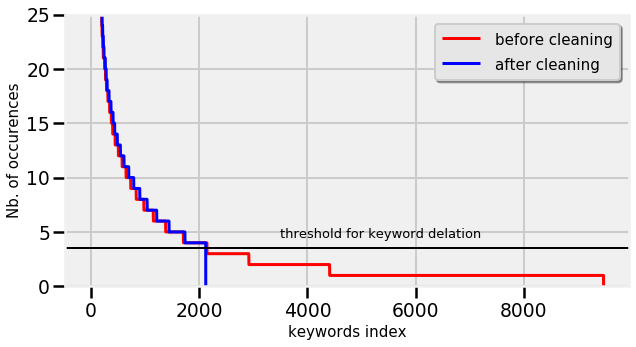
\includegraphics[height=10cm]{./contenido/imagenes/output_64_1.png}
\end{figure}

    { \hspace*{\fill} \\}
    
    \begin{center}\rule{0.5\linewidth}{\linethickness}\end{center}

\subsubsection{2.3 Correlaciones}\label{correlaciones}

    \begin{tcolorbox}[breakable, size=fbox, boxrule=1pt, pad at break*=1mm,colback=cellbackground, colframe=cellborder]
\prompt{In}{incolor}{49}{\hspace{4pt}}
\begin{Verbatim}[commandchars=\\\{\}]
\PY{n}{f}\PY{p}{,} \PY{n}{ax} \PY{o}{=} \PY{n}{plt}\PY{o}{.}\PY{n}{subplots}\PY{p}{(}\PY{n}{figsize}\PY{o}{=}\PY{p}{(}\PY{l+m+mi}{12}\PY{p}{,} \PY{l+m+mi}{9}\PY{p}{)}\PY{p}{)}
\PY{c+c1}{\PYZsh{}\PYZus{}\PYZus{}\PYZus{}\PYZus{}\PYZus{}\PYZus{}\PYZus{}\PYZus{}\PYZus{}\PYZus{}\PYZus{}\PYZus{}\PYZus{}\PYZus{}\PYZus{}\PYZus{}\PYZus{}\PYZus{}\PYZus{}\PYZus{}\PYZus{}\PYZus{}\PYZus{}\PYZus{}\PYZus{}\PYZus{}\PYZus{}\PYZus{}\PYZus{}}
\PY{c+c1}{\PYZsh{} Cálculo de correlaciones}
\PY{n}{corrmat} \PY{o}{=} \PY{n}{df\PYZus{}keywords\PYZus{}occurence}\PY{o}{.}\PY{n}{dropna}\PY{p}{(}\PY{n}{how}\PY{o}{=}\PY{l+s+s1}{\PYZsq{}}\PY{l+s+s1}{any}\PY{l+s+s1}{\PYZsq{}}\PY{p}{)}\PY{o}{.}\PY{n}{corr}\PY{p}{(}\PY{p}{)}
\PY{c+c1}{\PYZsh{}\PYZus{}\PYZus{}\PYZus{}\PYZus{}\PYZus{}\PYZus{}\PYZus{}\PYZus{}\PYZus{}\PYZus{}\PYZus{}\PYZus{}\PYZus{}\PYZus{}\PYZus{}\PYZus{}\PYZus{}\PYZus{}\PYZus{}\PYZus{}\PYZus{}\PYZus{}\PYZus{}\PYZus{}\PYZus{}\PYZus{}\PYZus{}\PYZus{}\PYZus{}\PYZus{}\PYZus{}\PYZus{}\PYZus{}\PYZus{}\PYZus{}\PYZus{}\PYZus{}\PYZus{}\PYZus{}\PYZus{}}
\PY{n}{k} \PY{o}{=} \PY{l+m+mi}{17} \PY{c+c1}{\PYZsh{} number of variables for heatmap}
\PY{n}{cols} \PY{o}{=} \PY{n}{corrmat}\PY{o}{.}\PY{n}{nlargest}\PY{p}{(}\PY{n}{k}\PY{p}{,} \PY{l+s+s1}{\PYZsq{}}\PY{l+s+s1}{num\PYZus{}voted\PYZus{}users}\PY{l+s+s1}{\PYZsq{}}\PY{p}{)}\PY{p}{[}\PY{l+s+s1}{\PYZsq{}}\PY{l+s+s1}{num\PYZus{}voted\PYZus{}users}\PY{l+s+s1}{\PYZsq{}}\PY{p}{]}\PY{o}{.}\PY{n}{index}
\PY{n}{cm} \PY{o}{=} \PY{n}{np}\PY{o}{.}\PY{n}{corrcoef}\PY{p}{(}\PY{n}{df\PYZus{}keywords\PYZus{}occurence}\PY{p}{[}\PY{n}{cols}\PY{p}{]}\PY{o}{.}\PY{n}{dropna}\PY{p}{(}\PY{n}{how}\PY{o}{=}\PY{l+s+s1}{\PYZsq{}}\PY{l+s+s1}{any}\PY{l+s+s1}{\PYZsq{}}\PY{p}{)}\PY{o}{.}\PY{n}{values}\PY{o}{.}\PY{n}{T}\PY{p}{)}
\PY{n}{sns}\PY{o}{.}\PY{n}{set}\PY{p}{(}\PY{n}{font\PYZus{}scale}\PY{o}{=}\PY{l+m+mf}{1.25}\PY{p}{)}
\PY{n}{hm} \PY{o}{=} \PY{n}{sns}\PY{o}{.}\PY{n}{heatmap}\PY{p}{(}\PY{n}{cm}\PY{p}{,} \PY{n}{cbar}\PY{o}{=}\PY{k+kc}{True}\PY{p}{,} \PY{n}{annot}\PY{o}{=}\PY{k+kc}{True}\PY{p}{,} \PY{n}{square}\PY{o}{=}\PY{k+kc}{True}\PY{p}{,}
                 \PY{n}{fmt}\PY{o}{=}\PY{l+s+s1}{\PYZsq{}}\PY{l+s+s1}{.2f}\PY{l+s+s1}{\PYZsq{}}\PY{p}{,} \PY{n}{annot\PYZus{}kws}\PY{o}{=}\PY{p}{\PYZob{}}\PY{l+s+s1}{\PYZsq{}}\PY{l+s+s1}{size}\PY{l+s+s1}{\PYZsq{}}\PY{p}{:} \PY{l+m+mi}{10}\PY{p}{\PYZcb{}}\PY{p}{,} \PY{n}{linewidth} \PY{o}{=} \PY{l+m+mf}{0.1}\PY{p}{,} \PY{n}{cmap} \PY{o}{=} \PY{l+s+s1}{\PYZsq{}}\PY{l+s+s1}{coolwarm}\PY{l+s+s1}{\PYZsq{}}\PY{p}{,}
                 \PY{n}{yticklabels}\PY{o}{=}\PY{n}{cols}\PY{o}{.}\PY{n}{values}\PY{p}{,} \PY{n}{xticklabels}\PY{o}{=}\PY{n}{cols}\PY{o}{.}\PY{n}{values}\PY{p}{)}
\PY{n}{f}\PY{o}{.}\PY{n}{text}\PY{p}{(}\PY{l+m+mf}{0.5}\PY{p}{,} \PY{l+m+mf}{0.93}\PY{p}{,} \PY{l+s+s2}{\PYZdq{}}\PY{l+s+s2}{Coeficientes de correlación}\PY{l+s+s2}{\PYZdq{}}\PY{p}{,} \PY{n}{ha}\PY{o}{=}\PY{l+s+s1}{\PYZsq{}}\PY{l+s+s1}{center}\PY{l+s+s1}{\PYZsq{}}\PY{p}{,} \PY{n}{fontsize} \PY{o}{=} \PY{l+m+mi}{18}\PY{p}{,} \PY{n}{family}\PY{o}{=}\PY{l+s+s1}{\PYZsq{}}\PY{l+s+s1}{fantasy}\PY{l+s+s1}{\PYZsq{}}\PY{p}{)}
\PY{n}{plt}\PY{o}{.}\PY{n}{show}\PY{p}{(}\PY{p}{)}
\end{Verbatim}
\end{tcolorbox}

    \begin{Verbatim}[commandchars=\\\{\}]
findfont: Font family ['fantasy'] not found. Falling back to DejaVu Sans.
findfont: Font family ['fantasy'] not found. Falling back to DejaVu Sans.
\end{Verbatim}

    \begin{center}
    \adjustimage{max size={0.9\linewidth}{0.9\paperheight}}{./contenido/imagenes/output_66_1.png}
    \end{center}
    { \hspace*{\fill} \\}
    
    \begin{tcolorbox}[breakable, size=fbox, boxrule=1pt, pad at break*=1mm,colback=cellbackground, colframe=cellborder]
\prompt{In}{incolor}{50}{\hspace{4pt}}
\begin{Verbatim}[commandchars=\\\{\}]
\PY{n}{LOST\PYZus{}COLUMNS} \PY{o}{=} \PY{p}{[}
    \PY{l+s+s1}{\PYZsq{}}\PY{l+s+s1}{actor\PYZus{}1\PYZus{}facebook\PYZus{}likes}\PY{l+s+s1}{\PYZsq{}}\PY{p}{,}
    \PY{l+s+s1}{\PYZsq{}}\PY{l+s+s1}{actor\PYZus{}2\PYZus{}facebook\PYZus{}likes}\PY{l+s+s1}{\PYZsq{}}\PY{p}{,}
    \PY{l+s+s1}{\PYZsq{}}\PY{l+s+s1}{actor\PYZus{}3\PYZus{}facebook\PYZus{}likes}\PY{l+s+s1}{\PYZsq{}}\PY{p}{,}
    \PY{l+s+s1}{\PYZsq{}}\PY{l+s+s1}{aspect\PYZus{}ratio}\PY{l+s+s1}{\PYZsq{}}\PY{p}{,}
    \PY{l+s+s1}{\PYZsq{}}\PY{l+s+s1}{cast\PYZus{}total\PYZus{}facebook\PYZus{}likes}\PY{l+s+s1}{\PYZsq{}}\PY{p}{,}
    \PY{l+s+s1}{\PYZsq{}}\PY{l+s+s1}{color}\PY{l+s+s1}{\PYZsq{}}\PY{p}{,}
    \PY{l+s+s1}{\PYZsq{}}\PY{l+s+s1}{content\PYZus{}rating}\PY{l+s+s1}{\PYZsq{}}\PY{p}{,}
    \PY{l+s+s1}{\PYZsq{}}\PY{l+s+s1}{director\PYZus{}facebook\PYZus{}likes}\PY{l+s+s1}{\PYZsq{}}\PY{p}{,}
    \PY{l+s+s1}{\PYZsq{}}\PY{l+s+s1}{facenumber\PYZus{}in\PYZus{}poster}\PY{l+s+s1}{\PYZsq{}}\PY{p}{,}
    \PY{l+s+s1}{\PYZsq{}}\PY{l+s+s1}{movie\PYZus{}facebook\PYZus{}likes}\PY{l+s+s1}{\PYZsq{}}\PY{p}{,}
    \PY{l+s+s1}{\PYZsq{}}\PY{l+s+s1}{movie\PYZus{}imdb\PYZus{}link}\PY{l+s+s1}{\PYZsq{}}\PY{p}{,}
    \PY{l+s+s1}{\PYZsq{}}\PY{l+s+s1}{num\PYZus{}critic\PYZus{}for\PYZus{}reviews}\PY{l+s+s1}{\PYZsq{}}\PY{p}{,}
    \PY{l+s+s1}{\PYZsq{}}\PY{l+s+s1}{num\PYZus{}user\PYZus{}for\PYZus{}reviews}\PY{l+s+s1}{\PYZsq{}}
                \PY{p}{]}
\end{Verbatim}
\end{tcolorbox}

    \begin{tcolorbox}[breakable, size=fbox, boxrule=1pt, pad at break*=1mm,colback=cellbackground, colframe=cellborder]
\prompt{In}{incolor}{51}{\hspace{4pt}}
\begin{Verbatim}[commandchars=\\\{\}]
\PY{c+c1}{\PYZsh{}\PYZus{}\PYZus{}\PYZus{}\PYZus{}\PYZus{}\PYZus{}\PYZus{}\PYZus{}\PYZus{}\PYZus{}}
\PY{c+c1}{\PYZsh{} dropping}
\PY{c+c1}{\PYZsh{}dropped\PYZus{}var = [\PYZsq{}aspect\PYZus{}ratio\PYZsq{}, \PYZsq{}budget\PYZsq{}, \PYZsq{}facenumber\PYZus{}in\PYZus{}poster\PYZsq{},}
\PY{c+c1}{\PYZsh{}               \PYZsq{}content\PYZus{}rating\PYZsq{}, \PYZsq{}cast\PYZus{}total\PYZus{}facebook\PYZus{}likes\PYZsq{}]}
\PY{c+c1}{\PYZsh{}df\PYZus{}var\PYZus{}cleaned = df\PYZus{}keywords\PYZus{}occurence.drop(dropped\PYZus{}var, axis = 1)}
\PY{c+c1}{\PYZsh{}\PYZus{}\PYZus{}\PYZus{}\PYZus{}\PYZus{}\PYZus{}\PYZus{}\PYZus{}\PYZus{}\PYZus{}\PYZus{}\PYZus{}\PYZus{}\PYZus{}\PYZus{}\PYZus{}}
\PY{c+c1}{\PYZsh{} and reordering}
\PY{n}{new\PYZus{}col\PYZus{}order} \PY{o}{=} \PY{p}{[}\PY{l+s+s1}{\PYZsq{}}\PY{l+s+s1}{movie\PYZus{}title}\PY{l+s+s1}{\PYZsq{}}\PY{p}{,} \PY{l+s+s1}{\PYZsq{}}\PY{l+s+s1}{title\PYZus{}year}\PY{l+s+s1}{\PYZsq{}}\PY{p}{,} \PY{l+s+s1}{\PYZsq{}}\PY{l+s+s1}{genres}\PY{l+s+s1}{\PYZsq{}}\PY{p}{,} \PY{l+s+s1}{\PYZsq{}}\PY{l+s+s1}{plot\PYZus{}keywords}\PY{l+s+s1}{\PYZsq{}}\PY{p}{,} 
                 \PY{l+s+s1}{\PYZsq{}}\PY{l+s+s1}{director\PYZus{}name}\PY{l+s+s1}{\PYZsq{}}\PY{p}{,} \PY{l+s+s1}{\PYZsq{}}\PY{l+s+s1}{actor\PYZus{}1\PYZus{}name}\PY{l+s+s1}{\PYZsq{}}\PY{p}{,} \PY{l+s+s1}{\PYZsq{}}\PY{l+s+s1}{actor\PYZus{}2\PYZus{}name}\PY{l+s+s1}{\PYZsq{}}\PY{p}{,} \PY{l+s+s1}{\PYZsq{}}\PY{l+s+s1}{actor\PYZus{}3\PYZus{}name}\PY{l+s+s1}{\PYZsq{}}\PY{p}{,}
                 \PY{l+s+s1}{\PYZsq{}}\PY{l+s+s1}{director\PYZus{}facebook\PYZus{}likes}\PY{l+s+s1}{\PYZsq{}}\PY{p}{,} \PY{l+s+s1}{\PYZsq{}}\PY{l+s+s1}{actor\PYZus{}1\PYZus{}facebook\PYZus{}likes}\PY{l+s+s1}{\PYZsq{}}\PY{p}{,} \PY{l+s+s1}{\PYZsq{}}\PY{l+s+s1}{actor\PYZus{}2\PYZus{}facebook\PYZus{}likes}\PY{l+s+s1}{\PYZsq{}}\PY{p}{,}
                 \PY{l+s+s1}{\PYZsq{}}\PY{l+s+s1}{actor\PYZus{}3\PYZus{}facebook\PYZus{}likes}\PY{l+s+s1}{\PYZsq{}}\PY{p}{,} \PY{l+s+s1}{\PYZsq{}}\PY{l+s+s1}{movie\PYZus{}facebook\PYZus{}likes}\PY{l+s+s1}{\PYZsq{}}\PY{p}{,} \PY{l+s+s1}{\PYZsq{}}\PY{l+s+s1}{num\PYZus{}critic\PYZus{}for\PYZus{}reviews}\PY{l+s+s1}{\PYZsq{}}\PY{p}{,} 
                 \PY{l+s+s1}{\PYZsq{}}\PY{l+s+s1}{num\PYZus{}user\PYZus{}for\PYZus{}reviews}\PY{l+s+s1}{\PYZsq{}}\PY{p}{,} \PY{l+s+s1}{\PYZsq{}}\PY{l+s+s1}{num\PYZus{}voted\PYZus{}users}\PY{l+s+s1}{\PYZsq{}}\PY{p}{,} \PY{l+s+s1}{\PYZsq{}}\PY{l+s+s1}{language}\PY{l+s+s1}{\PYZsq{}}\PY{p}{,} \PY{l+s+s1}{\PYZsq{}}\PY{l+s+s1}{country}\PY{l+s+s1}{\PYZsq{}}\PY{p}{,}
                 \PY{l+s+s1}{\PYZsq{}}\PY{l+s+s1}{imdb\PYZus{}score}\PY{l+s+s1}{\PYZsq{}}\PY{p}{,} \PY{l+s+s1}{\PYZsq{}}\PY{l+s+s1}{movie\PYZus{}imdb\PYZus{}link}\PY{l+s+s1}{\PYZsq{}}\PY{p}{,} \PY{l+s+s1}{\PYZsq{}}\PY{l+s+s1}{color}\PY{l+s+s1}{\PYZsq{}}\PY{p}{,} \PY{l+s+s1}{\PYZsq{}}\PY{l+s+s1}{duration}\PY{l+s+s1}{\PYZsq{}}\PY{p}{,} \PY{l+s+s1}{\PYZsq{}}\PY{l+s+s1}{gross}\PY{l+s+s1}{\PYZsq{}}\PY{p}{,} \PY{p}{]}
\PY{n}{new\PYZus{}col\PYZus{}order} \PY{o}{=} \PY{p}{[}\PY{n}{col} \PY{k}{for} \PY{n}{col} \PY{o+ow}{in} \PY{n}{new\PYZus{}col\PYZus{}order} \PY{k}{if} \PY{n}{col} \PY{o+ow}{not} \PY{o+ow}{in} \PY{n}{LOST\PYZus{}COLUMNS}\PY{p}{]}
\PY{n+nb}{print}\PY{p}{(}\PY{n}{new\PYZus{}col\PYZus{}order}\PY{p}{)}
\PY{n}{new\PYZus{}col\PYZus{}order} \PY{o}{=} \PY{p}{[}\PY{n}{IMDB\PYZus{}COLUMNS\PYZus{}TO\PYZus{}REMAP}\PY{p}{[}\PY{n}{col}\PY{p}{]} \PY{k}{if} \PY{n}{col} \PY{o+ow}{in} \PY{n}{IMDB\PYZus{}COLUMNS\PYZus{}TO\PYZus{}REMAP} \PY{k}{else} \PY{n}{col}
                 \PY{k}{for} \PY{n}{col} \PY{o+ow}{in} \PY{n}{new\PYZus{}col\PYZus{}order}\PY{p}{]}
\PY{n+nb}{print}\PY{p}{(}\PY{n}{new\PYZus{}col\PYZus{}order}\PY{p}{)}
\PY{n}{new\PYZus{}col\PYZus{}order} \PY{o}{=} \PY{p}{[}\PY{n}{TMDB\PYZus{}TO\PYZus{}IMDB\PYZus{}SIMPLE\PYZus{}EQUIVALENCIES}\PY{p}{[}\PY{n}{col}\PY{p}{]} \PY{k}{if} \PY{n}{col} \PY{o+ow}{in} \PY{n}{TMDB\PYZus{}TO\PYZus{}IMDB\PYZus{}SIMPLE\PYZus{}EQUIVALENCIES} \PY{k}{else} \PY{n}{col}
                 \PY{k}{for} \PY{n}{col} \PY{o+ow}{in} \PY{n}{new\PYZus{}col\PYZus{}order}\PY{p}{]}
\PY{n+nb}{print}\PY{p}{(}\PY{n}{new\PYZus{}col\PYZus{}order}\PY{p}{)}
\PY{n}{df\PYZus{}var\PYZus{}cleaned} \PY{o}{=} \PY{n}{df\PYZus{}keywords\PYZus{}occurence}\PY{p}{[}\PY{n}{new\PYZus{}col\PYZus{}order}\PY{p}{]}
\end{Verbatim}
\end{tcolorbox}

    \begin{Verbatim}[commandchars=\\\{\}]
['movie\_title', 'title\_year', 'genres', 'plot\_keywords', 'director\_name',
'actor\_1\_name', 'actor\_2\_name', 'actor\_3\_name', 'num\_voted\_users', 'language',
'country', 'imdb\_score', 'duration', 'gross']
['movie\_title', 'title\_year', 'genres', 'plot\_keywords', 'director\_name',
'actor\_1\_name', 'actor\_2\_name', 'actor\_3\_name', 'num\_voted\_users', 'language',
'country', 'vote\_average', 'duration', 'gross']
['movie\_title', 'title\_year', 'genres', 'plot\_keywords', 'director\_name',
'actor\_1\_name', 'actor\_2\_name', 'actor\_3\_name', 'num\_voted\_users', 'language',
'country', 'vote\_average', 'duration', 'gross']
\end{Verbatim}

    \begin{tcolorbox}[breakable, size=fbox, boxrule=1pt, pad at break*=1mm,colback=cellbackground, colframe=cellborder]
\prompt{In}{incolor}{52}{\hspace{4pt}}
\begin{Verbatim}[commandchars=\\\{\}]
\PY{n}{set2} \PY{o}{=} \PY{n+nb}{set}\PY{p}{(}\PY{n+nb}{list}\PY{p}{(}\PY{n}{df\PYZus{}var\PYZus{}cleaned}\PY{o}{.}\PY{n}{columns}\PY{p}{)}\PY{p}{)}
\end{Verbatim}
\end{tcolorbox}

    \begin{tcolorbox}[breakable, size=fbox, boxrule=1pt, pad at break*=1mm,colback=cellbackground, colframe=cellborder]
\prompt{In}{incolor}{53}{\hspace{4pt}}
\begin{Verbatim}[commandchars=\\\{\}]
\PY{n}{set1} \PY{o}{=} \PY{n+nb}{set}\PY{p}{(}\PY{n+nb}{list}\PY{p}{(}\PY{n}{df\PYZus{}keywords\PYZus{}occurence}\PY{o}{.}\PY{n}{columns}\PY{p}{)}\PY{p}{)}
\PY{n}{set1}\PY{o}{.}\PY{n}{difference}\PY{p}{(}\PY{n+nb}{list}\PY{p}{(}\PY{n}{df\PYZus{}var\PYZus{}cleaned}\PY{o}{.}\PY{n}{columns}\PY{p}{)}\PY{p}{)}
\end{Verbatim}
\end{tcolorbox}

            \begin{tcolorbox}[breakable, boxrule=.5pt, size=fbox, pad at break*=1mm, opacityfill=0]
\prompt{Out}{outcolor}{53}{\hspace{3.5pt}}
\begin{Verbatim}[commandchars=\\\{\}]
\{'budget',
 'homepage',
 'id',
 'original\_title',
 'overview',
 'popularity',
 'production\_companies',
 'production\_countries',
 'release\_date',
 'spoken\_languages',
 'status',
 'tagline'\}
\end{Verbatim}
\end{tcolorbox}
        
    \begin{center}\rule{0.5\linewidth}{\linethickness}\end{center}

\subsubsection{2.4 Valores faltantes}\label{valores-faltantes}

Examinamos el número de valores faltantes en cada variable y escogemos
una metodología para completar el dataset.

    \begin{tcolorbox}[breakable, size=fbox, boxrule=1pt, pad at break*=1mm,colback=cellbackground, colframe=cellborder]
\prompt{In}{incolor}{54}{\hspace{4pt}}
\begin{Verbatim}[commandchars=\\\{\}]
\PY{n}{missing\PYZus{}df} \PY{o}{=} \PY{n}{df\PYZus{}var\PYZus{}cleaned}\PY{o}{.}\PY{n}{isnull}\PY{p}{(}\PY{p}{)}\PY{o}{.}\PY{n}{sum}\PY{p}{(}\PY{n}{axis}\PY{o}{=}\PY{l+m+mi}{0}\PY{p}{)}\PY{o}{.}\PY{n}{reset\PYZus{}index}\PY{p}{(}\PY{p}{)}
\PY{n}{missing\PYZus{}df}\PY{o}{.}\PY{n}{columns} \PY{o}{=} \PY{p}{[}\PY{l+s+s1}{\PYZsq{}}\PY{l+s+s1}{column\PYZus{}name}\PY{l+s+s1}{\PYZsq{}}\PY{p}{,} \PY{l+s+s1}{\PYZsq{}}\PY{l+s+s1}{missing\PYZus{}count}\PY{l+s+s1}{\PYZsq{}}\PY{p}{]}
\PY{n}{missing\PYZus{}df}\PY{p}{[}\PY{l+s+s1}{\PYZsq{}}\PY{l+s+s1}{filling\PYZus{}factor}\PY{l+s+s1}{\PYZsq{}}\PY{p}{]} \PY{o}{=} \PY{p}{(}\PY{n}{df\PYZus{}var\PYZus{}cleaned}\PY{o}{.}\PY{n}{shape}\PY{p}{[}\PY{l+m+mi}{0}\PY{p}{]} 
                                \PY{o}{\PYZhy{}} \PY{n}{missing\PYZus{}df}\PY{p}{[}\PY{l+s+s1}{\PYZsq{}}\PY{l+s+s1}{missing\PYZus{}count}\PY{l+s+s1}{\PYZsq{}}\PY{p}{]}\PY{p}{)} \PY{o}{/} \PY{n}{df\PYZus{}var\PYZus{}cleaned}\PY{o}{.}\PY{n}{shape}\PY{p}{[}\PY{l+m+mi}{0}\PY{p}{]} \PY{o}{*} \PY{l+m+mi}{100}
\PY{n}{missing\PYZus{}df} \PY{o}{=} \PY{n}{missing\PYZus{}df}\PY{o}{.}\PY{n}{sort\PYZus{}values}\PY{p}{(}\PY{l+s+s1}{\PYZsq{}}\PY{l+s+s1}{filling\PYZus{}factor}\PY{l+s+s1}{\PYZsq{}}\PY{p}{)}\PY{o}{.}\PY{n}{reset\PYZus{}index}\PY{p}{(}\PY{n}{drop} \PY{o}{=} \PY{k+kc}{True}\PY{p}{)}
\PY{n}{missing\PYZus{}df}
\end{Verbatim}
\end{tcolorbox}

            \begin{tcolorbox}[breakable, boxrule=.5pt, size=fbox, pad at break*=1mm, opacityfill=0]
\prompt{Out}{outcolor}{54}{\hspace{3.5pt}}
\begin{Verbatim}[commandchars=\\\{\}]
        column\_name  missing\_count  filling\_factor
0           country            174       96.377264
1      actor\_3\_name             93       98.063710
2          language             86       98.209452
3      actor\_2\_name             63       98.688320
4      actor\_1\_name             53       98.896523
5     director\_name             30       99.375390
6          duration              2       99.958359
7        title\_year              1       99.979180
8       movie\_title              0      100.000000
9            genres              0      100.000000
10    plot\_keywords              0      100.000000
11  num\_voted\_users              0      100.000000
12     vote\_average              0      100.000000
13            gross              0      100.000000
\end{Verbatim}
\end{tcolorbox}
        
    Ahora representamos el contenido de esta tabla:

    \begin{tcolorbox}[breakable, size=fbox, boxrule=1pt, pad at break*=1mm,colback=cellbackground, colframe=cellborder]
\prompt{In}{incolor}{55}{\hspace{4pt}}
\begin{Verbatim}[commandchars=\\\{\}]
\PY{n}{y\PYZus{}axis} \PY{o}{=} \PY{n}{missing\PYZus{}df}\PY{p}{[}\PY{l+s+s1}{\PYZsq{}}\PY{l+s+s1}{filling\PYZus{}factor}\PY{l+s+s1}{\PYZsq{}}\PY{p}{]} 
\PY{n}{x\PYZus{}label} \PY{o}{=} \PY{n}{missing\PYZus{}df}\PY{p}{[}\PY{l+s+s1}{\PYZsq{}}\PY{l+s+s1}{column\PYZus{}name}\PY{l+s+s1}{\PYZsq{}}\PY{p}{]}
\PY{n}{x\PYZus{}axis} \PY{o}{=} \PY{n}{missing\PYZus{}df}\PY{o}{.}\PY{n}{index}

\PY{n}{fig} \PY{o}{=} \PY{n}{plt}\PY{o}{.}\PY{n}{figure}\PY{p}{(}\PY{n}{figsize}\PY{o}{=}\PY{p}{(}\PY{l+m+mi}{11}\PY{p}{,} \PY{l+m+mi}{4}\PY{p}{)}\PY{p}{)}
\PY{n}{plt}\PY{o}{.}\PY{n}{xticks}\PY{p}{(}\PY{n}{rotation}\PY{o}{=}\PY{l+m+mi}{80}\PY{p}{,} \PY{n}{fontsize} \PY{o}{=} \PY{l+m+mi}{14}\PY{p}{)}
\PY{n}{plt}\PY{o}{.}\PY{n}{yticks}\PY{p}{(}\PY{n}{fontsize} \PY{o}{=} \PY{l+m+mi}{13}\PY{p}{)}

\PY{n}{N\PYZus{}thresh} \PY{o}{=} \PY{l+m+mi}{5}
\PY{n}{plt}\PY{o}{.}\PY{n}{axvline}\PY{p}{(}\PY{n}{x}\PY{o}{=}\PY{n}{N\PYZus{}thresh}\PY{o}{\PYZhy{}}\PY{l+m+mf}{0.5}\PY{p}{,} \PY{n}{linewidth}\PY{o}{=}\PY{l+m+mi}{2}\PY{p}{,} \PY{n}{color} \PY{o}{=} \PY{l+s+s1}{\PYZsq{}}\PY{l+s+s1}{r}\PY{l+s+s1}{\PYZsq{}}\PY{p}{)}
\PY{n}{plt}\PY{o}{.}\PY{n}{text}\PY{p}{(}\PY{n}{N\PYZus{}thresh}\PY{o}{\PYZhy{}}\PY{l+m+mf}{4.8}\PY{p}{,} \PY{l+m+mi}{30}\PY{p}{,} \PY{l+s+s1}{\PYZsq{}}\PY{l+s+s1}{factor completitud }\PY{l+s+se}{\PYZbs{}n}\PY{l+s+s1}{ \PYZlt{} }\PY{l+s+si}{\PYZob{}\PYZcb{}}\PY{l+s+s1}{\PYZpc{}}\PY{l+s+s1}{\PYZsq{}}\PY{o}{.}\PY{n}{format}\PY{p}{(}\PY{n+nb}{round}\PY{p}{(}\PY{n}{y\PYZus{}axis}\PY{p}{[}\PY{n}{N\PYZus{}thresh}\PY{p}{]}\PY{p}{,}\PY{l+m+mi}{1}\PY{p}{)}\PY{p}{)}\PY{p}{,}
         \PY{n}{fontsize} \PY{o}{=} \PY{l+m+mi}{15}\PY{p}{,} \PY{n}{family} \PY{o}{=} \PY{l+s+s1}{\PYZsq{}}\PY{l+s+s1}{fantasy}\PY{l+s+s1}{\PYZsq{}}\PY{p}{,} \PY{n}{bbox}\PY{o}{=}\PY{n+nb}{dict}\PY{p}{(}\PY{n}{boxstyle}\PY{o}{=}\PY{l+s+s2}{\PYZdq{}}\PY{l+s+s2}{round}\PY{l+s+s2}{\PYZdq{}}\PY{p}{,}
                   \PY{n}{ec}\PY{o}{=}\PY{p}{(}\PY{l+m+mf}{1.0}\PY{p}{,} \PY{l+m+mf}{0.5}\PY{p}{,} \PY{l+m+mf}{0.5}\PY{p}{)}\PY{p}{,}
                   \PY{n}{fc}\PY{o}{=}\PY{p}{(}\PY{l+m+mf}{0.8}\PY{p}{,} \PY{l+m+mf}{0.5}\PY{p}{,} \PY{l+m+mf}{0.5}\PY{p}{)}\PY{p}{)}\PY{p}{)}
\PY{n}{N\PYZus{}thresh} \PY{o}{=} \PY{l+m+mi}{13}
\PY{n}{plt}\PY{o}{.}\PY{n}{axvline}\PY{p}{(}\PY{n}{x}\PY{o}{=}\PY{n}{N\PYZus{}thresh}\PY{o}{\PYZhy{}}\PY{l+m+mf}{0.5}\PY{p}{,} \PY{n}{linewidth}\PY{o}{=}\PY{l+m+mi}{2}\PY{p}{,} \PY{n}{color} \PY{o}{=} \PY{l+s+s1}{\PYZsq{}}\PY{l+s+s1}{g}\PY{l+s+s1}{\PYZsq{}}\PY{p}{)}
\PY{n}{plt}\PY{o}{.}\PY{n}{text}\PY{p}{(}\PY{n}{N\PYZus{}thresh}\PY{p}{,} \PY{l+m+mi}{30}\PY{p}{,} \PY{l+s+s1}{\PYZsq{}}\PY{l+s+s1}{factor completitud }\PY{l+s+se}{\PYZbs{}n}\PY{l+s+s1}{ = }\PY{l+s+si}{\PYZob{}\PYZcb{}}\PY{l+s+s1}{\PYZpc{}}\PY{l+s+s1}{\PYZsq{}}\PY{o}{.}\PY{n}{format}\PY{p}{(}\PY{n+nb}{round}\PY{p}{(}\PY{n}{y\PYZus{}axis}\PY{p}{[}\PY{n}{N\PYZus{}thresh}\PY{p}{]}\PY{p}{,}\PY{l+m+mi}{1}\PY{p}{)}\PY{p}{)}\PY{p}{,}
         \PY{n}{fontsize} \PY{o}{=} \PY{l+m+mi}{15}\PY{p}{,} \PY{n}{family} \PY{o}{=} \PY{l+s+s1}{\PYZsq{}}\PY{l+s+s1}{fantasy}\PY{l+s+s1}{\PYZsq{}}\PY{p}{,} \PY{n}{bbox}\PY{o}{=}\PY{n+nb}{dict}\PY{p}{(}\PY{n}{boxstyle}\PY{o}{=}\PY{l+s+s2}{\PYZdq{}}\PY{l+s+s2}{round}\PY{l+s+s2}{\PYZdq{}}\PY{p}{,}
                   \PY{n}{ec}\PY{o}{=}\PY{p}{(}\PY{l+m+mf}{1.}\PY{p}{,} \PY{l+m+mf}{0.5}\PY{p}{,} \PY{l+m+mf}{0.5}\PY{p}{)}\PY{p}{,}
                   \PY{n}{fc}\PY{o}{=}\PY{p}{(}\PY{l+m+mf}{0.5}\PY{p}{,} \PY{l+m+mf}{0.8}\PY{p}{,} \PY{l+m+mf}{0.5}\PY{p}{)}\PY{p}{)}\PY{p}{)}

\PY{n}{plt}\PY{o}{.}\PY{n}{xticks}\PY{p}{(}\PY{n}{x\PYZus{}axis}\PY{p}{,} \PY{n}{x\PYZus{}label}\PY{p}{,}\PY{n}{family}\PY{o}{=}\PY{l+s+s1}{\PYZsq{}}\PY{l+s+s1}{fantasy}\PY{l+s+s1}{\PYZsq{}}\PY{p}{,} \PY{n}{fontsize} \PY{o}{=} \PY{l+m+mi}{14} \PY{p}{)}
\PY{n}{plt}\PY{o}{.}\PY{n}{ylabel}\PY{p}{(}\PY{l+s+s1}{\PYZsq{}}\PY{l+s+s1}{Factor de completitud (}\PY{l+s+s1}{\PYZpc{}}\PY{l+s+s1}{)}\PY{l+s+s1}{\PYZsq{}}\PY{p}{,} \PY{n}{family}\PY{o}{=}\PY{l+s+s1}{\PYZsq{}}\PY{l+s+s1}{fantasy}\PY{l+s+s1}{\PYZsq{}}\PY{p}{,} \PY{n}{fontsize} \PY{o}{=} \PY{l+m+mi}{16}\PY{p}{)}
\PY{n}{plt}\PY{o}{.}\PY{n}{bar}\PY{p}{(}\PY{n}{x\PYZus{}axis}\PY{p}{,} \PY{n}{y\PYZus{}axis}\PY{p}{)}\PY{p}{;}
\end{Verbatim}
\end{tcolorbox}

    \begin{Verbatim}[commandchars=\\\{\}]
findfont: Font family ['fantasy'] not found. Falling back to DejaVu Sans.
findfont: Font family ['fantasy'] not found. Falling back to DejaVu Sans.
findfont: Font family ['fantasy'] not found. Falling back to DejaVu Sans.
\end{Verbatim}

\begin{figure}[h]
    \centering
    \captionsetup{width=10cm}
    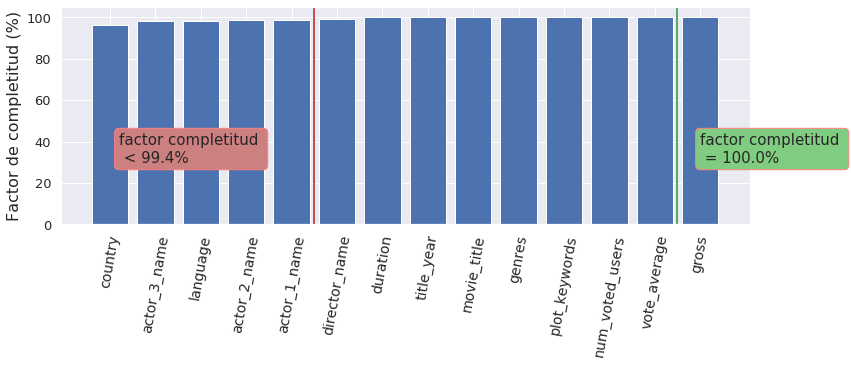
\includegraphics[height=10cm]{./contenido/imagenes/output_74_1.png}
\end{figure}
    { \hspace*{\fill} \\}
    
    \begin{center}\rule{0.5\linewidth}{\linethickness}\end{center}

\paragraph{2.4.1 Completando los años
faltantes}\label{completando-los-auxf1os-faltantes}

Para inferir el año de la película, se usan los actores y el director.
Para cada uno de ellos, determinamos el año medio de actividad,
utilizando el dataset que tenemos. A continuación, se promedian los
valores para determinar el año de la película.

To infer the title year, I use the list of actors and the director. For
each of them, I determine the mean year of activity, using the current
dataset. I then average the values obtained to estimate the title year.

    \begin{tcolorbox}[breakable, size=fbox, boxrule=1pt, pad at break*=1mm,colback=cellbackground, colframe=cellborder]
\prompt{In}{incolor}{56}{\hspace{4pt}}
\begin{Verbatim}[commandchars=\\\{\}]
\PY{n}{df\PYZus{}filling} \PY{o}{=} \PY{n}{df\PYZus{}var\PYZus{}cleaned}\PY{o}{.}\PY{n}{copy}\PY{p}{(}\PY{n}{deep}\PY{o}{=}\PY{k+kc}{True}\PY{p}{)}
\PY{n}{missing\PYZus{}year\PYZus{}info} \PY{o}{=} \PY{n}{df\PYZus{}filling}\PY{p}{[}\PY{n}{df\PYZus{}filling}\PY{p}{[}\PY{l+s+s1}{\PYZsq{}}\PY{l+s+s1}{title\PYZus{}year}\PY{l+s+s1}{\PYZsq{}}\PY{p}{]}\PY{o}{.}\PY{n}{isnull}\PY{p}{(}\PY{p}{)}\PY{p}{]}\PY{p}{[}\PY{p}{[}
            \PY{l+s+s1}{\PYZsq{}}\PY{l+s+s1}{director\PYZus{}name}\PY{l+s+s1}{\PYZsq{}}\PY{p}{,}\PY{l+s+s1}{\PYZsq{}}\PY{l+s+s1}{actor\PYZus{}1\PYZus{}name}\PY{l+s+s1}{\PYZsq{}}\PY{p}{,} \PY{l+s+s1}{\PYZsq{}}\PY{l+s+s1}{actor\PYZus{}2\PYZus{}name}\PY{l+s+s1}{\PYZsq{}}\PY{p}{,} \PY{l+s+s1}{\PYZsq{}}\PY{l+s+s1}{actor\PYZus{}3\PYZus{}name}\PY{l+s+s1}{\PYZsq{}}\PY{p}{]}\PY{p}{]}
\PY{n}{missing\PYZus{}year\PYZus{}info}\PY{p}{[}\PY{p}{:}\PY{l+m+mi}{10}\PY{p}{]}
\end{Verbatim}
\end{tcolorbox}

            \begin{tcolorbox}[breakable, boxrule=.5pt, size=fbox, pad at break*=1mm, opacityfill=0]
\prompt{Out}{outcolor}{56}{\hspace{3.5pt}}
\begin{Verbatim}[commandchars=\\\{\}]
     director\_name actor\_1\_name actor\_2\_name actor\_3\_name
4553           NaN          NaN          NaN          NaN
\end{Verbatim}
\end{tcolorbox}
        
    \begin{tcolorbox}[breakable, size=fbox, boxrule=1pt, pad at break*=1mm,colback=cellbackground, colframe=cellborder]
\prompt{In}{incolor}{57}{\hspace{4pt}}
\begin{Verbatim}[commandchars=\\\{\}]
\PY{k}{def} \PY{n+nf}{fill\PYZus{}year}\PY{p}{(}\PY{n}{df}\PY{p}{)}\PY{p}{:}
    \PY{l+s+sd}{\PYZdq{}\PYZdq{}\PYZdq{}Completa la columna faltante del año teniendo en cuenta la media}
\PY{l+s+sd}{    de los periodos de actividad de los actores y el director.}
\PY{l+s+sd}{    \PYZdq{}\PYZdq{}\PYZdq{}}
    \PY{n}{col} \PY{o}{=} \PY{p}{[}\PY{l+s+s1}{\PYZsq{}}\PY{l+s+s1}{director\PYZus{}name}\PY{l+s+s1}{\PYZsq{}}\PY{p}{,} \PY{l+s+s1}{\PYZsq{}}\PY{l+s+s1}{actor\PYZus{}1\PYZus{}name}\PY{l+s+s1}{\PYZsq{}}\PY{p}{,} \PY{l+s+s1}{\PYZsq{}}\PY{l+s+s1}{actor\PYZus{}2\PYZus{}name}\PY{l+s+s1}{\PYZsq{}}\PY{p}{,} \PY{l+s+s1}{\PYZsq{}}\PY{l+s+s1}{actor\PYZus{}3\PYZus{}name}\PY{l+s+s1}{\PYZsq{}}\PY{p}{]}
    \PY{n}{usual\PYZus{}year} \PY{o}{=} \PY{p}{[}\PY{l+m+mi}{0} \PY{k}{for} \PY{n}{\PYZus{}} \PY{o+ow}{in} \PY{n+nb}{range}\PY{p}{(}\PY{l+m+mi}{4}\PY{p}{)}\PY{p}{]}
    \PY{n}{var}        \PY{o}{=} \PY{p}{[}\PY{l+m+mi}{0} \PY{k}{for} \PY{n}{\PYZus{}} \PY{o+ow}{in} \PY{n+nb}{range}\PY{p}{(}\PY{l+m+mi}{4}\PY{p}{)}\PY{p}{]}
    \PY{c+c1}{\PYZsh{}\PYZus{}\PYZus{}\PYZus{}\PYZus{}\PYZus{}\PYZus{}\PYZus{}\PYZus{}\PYZus{}\PYZus{}\PYZus{}\PYZus{}\PYZus{}\PYZus{}\PYZus{}\PYZus{}\PYZus{}\PYZus{}\PYZus{}\PYZus{}\PYZus{}\PYZus{}\PYZus{}\PYZus{}\PYZus{}\PYZus{}\PYZus{}\PYZus{}\PYZus{}\PYZus{}\PYZus{}\PYZus{}\PYZus{}\PYZus{}\PYZus{}\PYZus{}\PYZus{}\PYZus{}\PYZus{}\PYZus{}\PYZus{}\PYZus{}\PYZus{}\PYZus{}\PYZus{}\PYZus{}\PYZus{}\PYZus{}\PYZus{}\PYZus{}\PYZus{}\PYZus{}\PYZus{}\PYZus{}\PYZus{}\PYZus{}\PYZus{}\PYZus{}\PYZus{}\PYZus{}\PYZus{}}
    \PY{c+c1}{\PYZsh{} Año medio de actividad para los actores y el director}
    \PY{k}{for} \PY{n}{i} \PY{o+ow}{in} \PY{n+nb}{range}\PY{p}{(}\PY{n+nb}{len}\PY{p}{(}\PY{n}{col}\PY{p}{)}\PY{p}{)}\PY{p}{:}
        \PY{n}{usual\PYZus{}year}\PY{p}{[}\PY{n}{i}\PY{p}{]} \PY{o}{=} \PY{n}{df}\PY{o}{.}\PY{n}{groupby}\PY{p}{(}\PY{n}{col}\PY{p}{[}\PY{n}{i}\PY{p}{]}\PY{p}{)}\PY{p}{[}\PY{l+s+s1}{\PYZsq{}}\PY{l+s+s1}{title\PYZus{}year}\PY{l+s+s1}{\PYZsq{}}\PY{p}{]}\PY{o}{.}\PY{n}{mean}\PY{p}{(}\PY{p}{)}
    \PY{c+c1}{\PYZsh{}\PYZus{}\PYZus{}\PYZus{}\PYZus{}\PYZus{}\PYZus{}\PYZus{}\PYZus{}\PYZus{}\PYZus{}\PYZus{}\PYZus{}\PYZus{}\PYZus{}\PYZus{}\PYZus{}\PYZus{}\PYZus{}\PYZus{}\PYZus{}\PYZus{}\PYZus{}\PYZus{}\PYZus{}\PYZus{}\PYZus{}\PYZus{}\PYZus{}\PYZus{}\PYZus{}\PYZus{}\PYZus{}\PYZus{}\PYZus{}\PYZus{}\PYZus{}\PYZus{}\PYZus{}\PYZus{}\PYZus{}\PYZus{}\PYZus{}\PYZus{}\PYZus{}\PYZus{}}
    \PY{c+c1}{\PYZsh{} Diccionario que recoja esta información}
    \PY{n}{actor\PYZus{}year} \PY{o}{=} \PY{n+nb}{dict}\PY{p}{(}\PY{p}{)}
    \PY{k}{for} \PY{n}{i} \PY{o+ow}{in} \PY{n+nb}{range}\PY{p}{(}\PY{l+m+mi}{4}\PY{p}{)}\PY{p}{:}
        \PY{k}{for} \PY{n}{s} \PY{o+ow}{in} \PY{n}{usual\PYZus{}year}\PY{p}{[}\PY{n}{i}\PY{p}{]}\PY{o}{.}\PY{n}{index}\PY{p}{:}
            \PY{k}{if} \PY{n}{s} \PY{o+ow}{in} \PY{n}{actor\PYZus{}year}\PY{o}{.}\PY{n}{keys}\PY{p}{(}\PY{p}{)}\PY{p}{:}
                \PY{k}{if} \PY{n}{pd}\PY{o}{.}\PY{n}{notnull}\PY{p}{(}\PY{n}{usual\PYZus{}year}\PY{p}{[}\PY{n}{i}\PY{p}{]}\PY{p}{[}\PY{n}{s}\PY{p}{]}\PY{p}{)} \PY{o+ow}{and} \PY{n}{pd}\PY{o}{.}\PY{n}{notnull}\PY{p}{(}\PY{n}{actor\PYZus{}year}\PY{p}{[}\PY{n}{s}\PY{p}{]}\PY{p}{)}\PY{p}{:}
                    \PY{n}{actor\PYZus{}year}\PY{p}{[}\PY{n}{s}\PY{p}{]} \PY{o}{=} \PY{p}{(}\PY{n}{actor\PYZus{}year}\PY{p}{[}\PY{n}{s}\PY{p}{]} \PY{o}{+} \PY{n}{usual\PYZus{}year}\PY{p}{[}\PY{n}{i}\PY{p}{]}\PY{p}{[}\PY{n}{s}\PY{p}{]}\PY{p}{)}\PY{o}{/}\PY{l+m+mi}{2}
                \PY{k}{elif} \PY{n}{pd}\PY{o}{.}\PY{n}{isnull}\PY{p}{(}\PY{n}{actor\PYZus{}year}\PY{p}{[}\PY{n}{s}\PY{p}{]}\PY{p}{)}\PY{p}{:}
                    \PY{n}{actor\PYZus{}year}\PY{p}{[}\PY{n}{s}\PY{p}{]} \PY{o}{=} \PY{n}{usual\PYZus{}year}\PY{p}{[}\PY{n}{i}\PY{p}{]}\PY{p}{[}\PY{n}{s}\PY{p}{]}
            \PY{k}{else}\PY{p}{:}
                \PY{n}{actor\PYZus{}year}\PY{p}{[}\PY{n}{s}\PY{p}{]} \PY{o}{=} \PY{n}{usual\PYZus{}year}\PY{p}{[}\PY{n}{i}\PY{p}{]}\PY{p}{[}\PY{n}{s}\PY{p}{]}
        
    \PY{c+c1}{\PYZsh{}\PYZus{}\PYZus{}\PYZus{}\PYZus{}\PYZus{}\PYZus{}\PYZus{}\PYZus{}\PYZus{}\PYZus{}\PYZus{}\PYZus{}\PYZus{}\PYZus{}\PYZus{}\PYZus{}\PYZus{}\PYZus{}\PYZus{}\PYZus{}\PYZus{}\PYZus{}\PYZus{}\PYZus{}\PYZus{}\PYZus{}\PYZus{}\PYZus{}\PYZus{}\PYZus{}\PYZus{}\PYZus{}\PYZus{}\PYZus{}\PYZus{}\PYZus{}\PYZus{}\PYZus{}}
    \PY{c+c1}{\PYZsh{} Identificación de los años faltantes}
    \PY{n}{missing\PYZus{}year\PYZus{}info} \PY{o}{=} \PY{n}{df}\PY{p}{[}\PY{n}{df}\PY{p}{[}\PY{l+s+s1}{\PYZsq{}}\PY{l+s+s1}{title\PYZus{}year}\PY{l+s+s1}{\PYZsq{}}\PY{p}{]}\PY{o}{.}\PY{n}{isnull}\PY{p}{(}\PY{p}{)}\PY{p}{]}
    \PY{c+c1}{\PYZsh{}\PYZus{}\PYZus{}\PYZus{}\PYZus{}\PYZus{}\PYZus{}\PYZus{}\PYZus{}\PYZus{}\PYZus{}\PYZus{}\PYZus{}\PYZus{}\PYZus{}\PYZus{}\PYZus{}\PYZus{}\PYZus{}\PYZus{}\PYZus{}\PYZus{}\PYZus{}\PYZus{}\PYZus{}\PYZus{}\PYZus{}\PYZus{}}
    \PY{c+c1}{\PYZsh{} Completado de los valores faltantes}
    \PY{n}{icount\PYZus{}replaced} \PY{o}{=} \PY{l+m+mi}{0}
    \PY{k}{for} \PY{n}{index}\PY{p}{,} \PY{n}{row} \PY{o+ow}{in} \PY{n}{missing\PYZus{}year\PYZus{}info}\PY{o}{.}\PY{n}{iterrows}\PY{p}{(}\PY{p}{)}\PY{p}{:}
        \PY{n}{value} \PY{o}{=} \PY{p}{[} \PY{n}{np}\PY{o}{.}\PY{n}{NaN} \PY{k}{for} \PY{n}{\PYZus{}} \PY{o+ow}{in} \PY{n+nb}{range}\PY{p}{(}\PY{l+m+mi}{4}\PY{p}{)}\PY{p}{]}
        \PY{n}{icount} \PY{o}{=} \PY{l+m+mi}{0} \PY{p}{;} \PY{n}{sum\PYZus{}year} \PY{o}{=} \PY{l+m+mi}{0}
        \PY{k}{for} \PY{n}{i} \PY{o+ow}{in} \PY{n+nb}{range}\PY{p}{(}\PY{l+m+mi}{4}\PY{p}{)}\PY{p}{:}            
            \PY{n}{var}\PY{p}{[}\PY{n}{i}\PY{p}{]} \PY{o}{=} \PY{n}{df}\PY{o}{.}\PY{n}{loc}\PY{p}{[}\PY{n}{index}\PY{p}{]}\PY{p}{[}\PY{n}{col}\PY{p}{[}\PY{n}{i}\PY{p}{]}\PY{p}{]}
            \PY{k}{if} \PY{n}{pd}\PY{o}{.}\PY{n}{notnull}\PY{p}{(}\PY{n}{var}\PY{p}{[}\PY{n}{i}\PY{p}{]}\PY{p}{)}\PY{p}{:} \PY{n}{value}\PY{p}{[}\PY{n}{i}\PY{p}{]} \PY{o}{=} \PY{n}{actor\PYZus{}year}\PY{p}{[}\PY{n}{var}\PY{p}{[}\PY{n}{i}\PY{p}{]}\PY{p}{]}
            \PY{k}{if} \PY{n}{pd}\PY{o}{.}\PY{n}{notnull}\PY{p}{(}\PY{n}{value}\PY{p}{[}\PY{n}{i}\PY{p}{]}\PY{p}{)}\PY{p}{:} \PY{n}{icount} \PY{o}{+}\PY{o}{=} \PY{l+m+mi}{1} \PY{p}{;} \PY{n}{sum\PYZus{}year} \PY{o}{+}\PY{o}{=} \PY{n}{actor\PYZus{}year}\PY{p}{[}\PY{n}{var}\PY{p}{[}\PY{n}{i}\PY{p}{]}\PY{p}{]}
        \PY{k}{if} \PY{n}{icount} \PY{o}{!=} \PY{l+m+mi}{0}\PY{p}{:} \PY{n}{sum\PYZus{}year} \PY{o}{=} \PY{n}{sum\PYZus{}year} \PY{o}{/} \PY{n}{icount} 

        \PY{k}{if} \PY{n+nb}{int}\PY{p}{(}\PY{n}{sum\PYZus{}year}\PY{p}{)} \PY{o}{\PYZgt{}} \PY{l+m+mi}{0}\PY{p}{:}
            \PY{n}{icount\PYZus{}replaced} \PY{o}{+}\PY{o}{=} \PY{l+m+mi}{1}
            \PY{n}{df}\PY{o}{.}\PY{n}{set\PYZus{}value}\PY{p}{(}\PY{n}{index}\PY{p}{,} \PY{l+s+s1}{\PYZsq{}}\PY{l+s+s1}{title\PYZus{}year}\PY{l+s+s1}{\PYZsq{}}\PY{p}{,} \PY{n+nb}{int}\PY{p}{(}\PY{n}{sum\PYZus{}year}\PY{p}{)}\PY{p}{)}
            \PY{k}{if} \PY{n}{icount\PYZus{}replaced} \PY{o}{\PYZlt{}} \PY{l+m+mi}{10}\PY{p}{:} 
                \PY{n+nb}{print}\PY{p}{(}\PY{l+s+s2}{\PYZdq{}}\PY{l+s+si}{\PYZob{}:\PYZlt{}45\PYZcb{}}\PY{l+s+s2}{ \PYZhy{}\PYZgt{} }\PY{l+s+si}{\PYZob{}:\PYZlt{}20\PYZcb{}}\PY{l+s+s2}{\PYZdq{}}\PY{o}{.}\PY{n}{format}\PY{p}{(}\PY{n}{df}\PY{o}{.}\PY{n}{loc}\PY{p}{[}\PY{n}{index}\PY{p}{]}\PY{p}{[}\PY{l+s+s1}{\PYZsq{}}\PY{l+s+s1}{movie\PYZus{}title}\PY{l+s+s1}{\PYZsq{}}\PY{p}{]}\PY{p}{,}\PY{n+nb}{int}\PY{p}{(}\PY{n}{sum\PYZus{}year}\PY{p}{)}\PY{p}{)}\PY{p}{)}
    \PY{k}{return} 
\end{Verbatim}
\end{tcolorbox}

    \begin{tcolorbox}[breakable, size=fbox, boxrule=1pt, pad at break*=1mm,colback=cellbackground, colframe=cellborder]
\prompt{In}{incolor}{58}{\hspace{4pt}}
\begin{Verbatim}[commandchars=\\\{\}]
\PY{n}{fill\PYZus{}year}\PY{p}{(}\PY{n}{df\PYZus{}filling}\PY{p}{)}
\end{Verbatim}
\end{tcolorbox}

    \paragraph{La comparación de algunas predicciones con valores reales
presentan un grado de similaridad relativamente
bueno}\label{la-comparaciuxf3n-de-algunas-predicciones-con-valores-reales-presentan-un-grado-de-similaridad-relativamente-bueno}

\begin{itemize}
\tightlist
\item
  Bewitched: \textbf{1951} -\textgreater{} en TV entre 1964 y 1972
\item
  The A-team: \textbf{1977} -\textgreater{} en TV entre 1982 y 1987
\item
  Sleepy Hollow: \textbf{2012} -\textgreater{} en TV entre 2013 y 2017
\end{itemize}

    \begin{center}\rule{0.5\linewidth}{\linethickness}\end{center}

\paragraph{2.4.2 Extracción de keywords del
título}\label{extracciuxf3n-de-keywords-del-tuxedtulo}

Como se ha dicho anteriormente, las keywords jugarán un papel
fundamental en el funcionamiento del motor de recomendación. Por tanto,
se tratará de rellenar los valores faltantes de la variable
\textbf{plot\_keywords} utilizando keywords del título. Para ello, se
crea la lista de sinónimos de todas las palabras contenidas en el título
y se comprueba si alguna de ellas se encuentra ya en la lista de
keywords. En ese caso, se añade esa keyword a la película.

    \begin{tcolorbox}[breakable, size=fbox, boxrule=1pt, pad at break*=1mm,colback=cellbackground, colframe=cellborder]
\prompt{In}{incolor}{59}{\hspace{4pt}}
\begin{Verbatim}[commandchars=\\\{\}]
\PY{n}{icount} \PY{o}{=} \PY{l+m+mi}{0}
\PY{k}{for} \PY{n}{index}\PY{p}{,} \PY{n}{row} \PY{o+ow}{in} \PY{n}{df\PYZus{}filling}\PY{p}{[}\PY{n}{df\PYZus{}filling}\PY{p}{[}\PY{l+s+s1}{\PYZsq{}}\PY{l+s+s1}{plot\PYZus{}keywords}\PY{l+s+s1}{\PYZsq{}}\PY{p}{]}\PY{o}{.}\PY{n}{isnull}\PY{p}{(}\PY{p}{)}\PY{p}{]}\PY{o}{.}\PY{n}{iterrows}\PY{p}{(}\PY{p}{)}\PY{p}{:}
    \PY{n}{icount} \PY{o}{+}\PY{o}{=} \PY{l+m+mi}{1}
    \PY{n}{word\PYZus{}list} \PY{o}{=} \PY{n}{row}\PY{p}{[}\PY{l+s+s1}{\PYZsq{}}\PY{l+s+s1}{movie\PYZus{}title}\PY{l+s+s1}{\PYZsq{}}\PY{p}{]}\PY{o}{.}\PY{n}{strip}\PY{p}{(}\PY{p}{)}\PY{o}{.}\PY{n}{split}\PY{p}{(}\PY{p}{)}
    \PY{n}{new\PYZus{}keyword} \PY{o}{=} \PY{p}{[}\PY{p}{]}
    \PY{k}{for} \PY{n}{s} \PY{o+ow}{in} \PY{n}{word\PYZus{}list}\PY{p}{:}
        \PY{n}{lemma} \PY{o}{=} \PY{n}{get\PYZus{}synonyms}\PY{p}{(}\PY{n}{s}\PY{p}{)}
        \PY{k}{for} \PY{n}{t} \PY{o+ow}{in} \PY{n+nb}{list}\PY{p}{(}\PY{n}{lemma}\PY{p}{)}\PY{p}{:}
            \PY{k}{if} \PY{n}{t} \PY{o+ow}{in} \PY{n}{keywords}\PY{p}{:} 
                \PY{n}{new\PYZus{}keyword}\PY{o}{.}\PY{n}{append}\PY{p}{(}\PY{n}{t}\PY{p}{)}                
    \PY{k}{if} \PY{n}{new\PYZus{}keyword} \PY{o+ow}{and} \PY{n}{icount} \PY{o}{\PYZlt{}} \PY{l+m+mi}{15}\PY{p}{:} 
        \PY{n+nb}{print}\PY{p}{(}\PY{l+s+s1}{\PYZsq{}}\PY{l+s+si}{\PYZob{}:\PYZlt{}50\PYZcb{}}\PY{l+s+s1}{ \PYZhy{}\PYZgt{} }\PY{l+s+si}{\PYZob{}:\PYZlt{}30\PYZcb{}}\PY{l+s+s1}{\PYZsq{}}\PY{o}{.}\PY{n}{format}\PY{p}{(}\PY{n}{row}\PY{p}{[}\PY{l+s+s1}{\PYZsq{}}\PY{l+s+s1}{movie\PYZus{}title}\PY{l+s+s1}{\PYZsq{}}\PY{p}{]}\PY{p}{,} \PY{n+nb}{str}\PY{p}{(}\PY{n}{new\PYZus{}keyword}\PY{p}{)}\PY{p}{)}\PY{p}{)}
    \PY{k}{if} \PY{n}{new\PYZus{}keyword}\PY{p}{:}
        \PY{n}{df\PYZus{}filling}\PY{o}{.}\PY{n}{set\PYZus{}value}\PY{p}{(}\PY{n}{index}\PY{p}{,} \PY{l+s+s1}{\PYZsq{}}\PY{l+s+s1}{plot\PYZus{}keywords}\PY{l+s+s1}{\PYZsq{}}\PY{p}{,} \PY{l+s+s1}{\PYZsq{}}\PY{l+s+s1}{|}\PY{l+s+s1}{\PYZsq{}}\PY{o}{.}\PY{n}{join}\PY{p}{(}\PY{n}{new\PYZus{}keyword}\PY{p}{)}\PY{p}{)} 
\end{Verbatim}
\end{tcolorbox}

    \paragraph{2.4.3 Completando mediante regresionesImputing from
regressions}\label{completando-mediante-regresionesimputing-from-regressions}

En la sección 2.4 se vio la correlación entre variabels y se encontro
que algunas de ellas tenían una cierta correlación, con un coeficiente
de Pearson \(>0.5\):

    \begin{tcolorbox}[breakable, size=fbox, boxrule=1pt, pad at break*=1mm,colback=cellbackground, colframe=cellborder]
\prompt{In}{incolor}{60}{\hspace{4pt}}
\begin{Verbatim}[commandchars=\\\{\}]
\PY{n}{cols} \PY{o}{=} \PY{n}{corrmat}\PY{o}{.}\PY{n}{nlargest}\PY{p}{(}\PY{l+m+mi}{9}\PY{p}{,} \PY{l+s+s1}{\PYZsq{}}\PY{l+s+s1}{num\PYZus{}voted\PYZus{}users}\PY{l+s+s1}{\PYZsq{}}\PY{p}{)}\PY{p}{[}\PY{l+s+s1}{\PYZsq{}}\PY{l+s+s1}{num\PYZus{}voted\PYZus{}users}\PY{l+s+s1}{\PYZsq{}}\PY{p}{]}\PY{o}{.}\PY{n}{index}
\PY{n}{cm} \PY{o}{=} \PY{n}{np}\PY{o}{.}\PY{n}{corrcoef}\PY{p}{(}\PY{n}{df\PYZus{}keywords\PYZus{}occurence}\PY{p}{[}\PY{n}{cols}\PY{p}{]}\PY{o}{.}\PY{n}{dropna}\PY{p}{(}\PY{n}{how}\PY{o}{=}\PY{l+s+s1}{\PYZsq{}}\PY{l+s+s1}{any}\PY{l+s+s1}{\PYZsq{}}\PY{p}{)}\PY{o}{.}\PY{n}{values}\PY{o}{.}\PY{n}{T}\PY{p}{)}
\PY{n}{sns}\PY{o}{.}\PY{n}{set}\PY{p}{(}\PY{n}{font\PYZus{}scale}\PY{o}{=}\PY{l+m+mf}{1.25}\PY{p}{)}
\PY{n}{hm} \PY{o}{=} \PY{n}{sns}\PY{o}{.}\PY{n}{heatmap}\PY{p}{(}\PY{n}{cm}\PY{p}{,} \PY{n}{cbar}\PY{o}{=}\PY{k+kc}{True}\PY{p}{,} \PY{n}{annot}\PY{o}{=}\PY{k+kc}{True}\PY{p}{,} \PY{n}{square}\PY{o}{=}\PY{k+kc}{True}\PY{p}{,}
                 \PY{n}{fmt}\PY{o}{=}\PY{l+s+s1}{\PYZsq{}}\PY{l+s+s1}{.2f}\PY{l+s+s1}{\PYZsq{}}\PY{p}{,} \PY{n}{annot\PYZus{}kws}\PY{o}{=}\PY{p}{\PYZob{}}\PY{l+s+s1}{\PYZsq{}}\PY{l+s+s1}{size}\PY{l+s+s1}{\PYZsq{}}\PY{p}{:} \PY{l+m+mi}{10}\PY{p}{\PYZcb{}}\PY{p}{,} 
                 \PY{n}{yticklabels}\PY{o}{=}\PY{n}{cols}\PY{o}{.}\PY{n}{values}\PY{p}{,} \PY{n}{xticklabels}\PY{o}{=}\PY{n}{cols}\PY{o}{.}\PY{n}{values}\PY{p}{)}
\PY{n}{plt}\PY{o}{.}\PY{n}{show}\PY{p}{(}\PY{p}{)}
\end{Verbatim}
\end{tcolorbox}

\begin{figure}[h]
    \centering
    \captionsetup{width=10cm}
    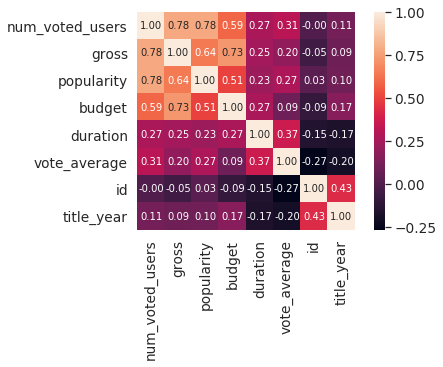
\includegraphics[height=10cm]{./contenido/imagenes/output_83_0.png}
\end{figure}

    { \hspace*{\fill} \\}
    
    Se usará este hallazgo para completar los valores faltantes de las
variables \textbf{gross} y \textbf{num\_voted\_users}. Para ello, se
realizarán regresiones en parejas de variables correlacionadas:

    \begin{tcolorbox}[breakable, size=fbox, boxrule=1pt, pad at break*=1mm,colback=cellbackground, colframe=cellborder]
\prompt{In}{incolor}{61}{\hspace{4pt}}
\begin{Verbatim}[commandchars=\\\{\}]
\PY{n}{sns}\PY{o}{.}\PY{n}{set}\PY{p}{(}\PY{n}{font\PYZus{}scale}\PY{o}{=}\PY{l+m+mf}{1.25}\PY{p}{)}
\PY{c+c1}{\PYZsh{}cols = [\PYZsq{}gross\PYZsq{}, \PYZsq{}num\PYZus{}voted\PYZus{}users\PYZsq{}, \PYZsq{}num\PYZus{}critic\PYZus{}for\PYZus{}reviews\PYZsq{}, \PYZsq{}num\PYZus{}user\PYZus{}for\PYZus{}reviews\PYZsq{}]}
\PY{n}{cols} \PY{o}{=} \PY{p}{[}\PY{l+s+s1}{\PYZsq{}}\PY{l+s+s1}{gross}\PY{l+s+s1}{\PYZsq{}}\PY{p}{,} \PY{l+s+s1}{\PYZsq{}}\PY{l+s+s1}{num\PYZus{}voted\PYZus{}users}\PY{l+s+s1}{\PYZsq{}}\PY{p}{]}
\PY{n}{sns}\PY{o}{.}\PY{n}{pairplot}\PY{p}{(}\PY{n}{df\PYZus{}filling}\PY{o}{.}\PY{n}{dropna}\PY{p}{(}\PY{n}{how}\PY{o}{=}\PY{l+s+s1}{\PYZsq{}}\PY{l+s+s1}{any}\PY{l+s+s1}{\PYZsq{}}\PY{p}{)}\PY{p}{[}\PY{n}{cols}\PY{p}{]}\PY{p}{,}\PY{n}{diag\PYZus{}kind}\PY{o}{=}\PY{l+s+s1}{\PYZsq{}}\PY{l+s+s1}{kde}\PY{l+s+s1}{\PYZsq{}}\PY{p}{,} \PY{n}{size} \PY{o}{=} \PY{l+m+mf}{2.5}\PY{p}{)}
\PY{n}{plt}\PY{o}{.}\PY{n}{show}\PY{p}{(}\PY{p}{)}\PY{p}{;}
\end{Verbatim}
\end{tcolorbox}
\begin{figure}[h]
    \centering
    \captionsetup{width=10cm}
    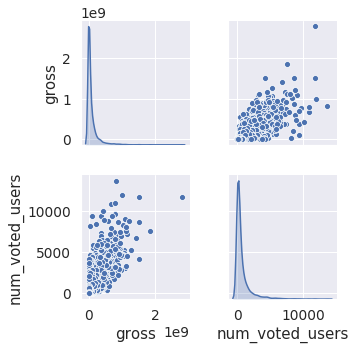
\includegraphics[height=10cm]{./contenido/imagenes/output_85_0.png}
\end{figure}

    { \hspace*{\fill} \\}
    
    En primer lugar, definimos una función que imputa los vbalores faltantes
mediante un ajuste lineal de los datos:

    \begin{tcolorbox}[breakable, size=fbox, boxrule=1pt, pad at break*=1mm,colback=cellbackground, colframe=cellborder]
\prompt{In}{incolor}{64}{\hspace{4pt}}
\begin{Verbatim}[commandchars=\\\{\}]
\PY{k}{def} \PY{n+nf}{variable\PYZus{}linreg\PYZus{}imputation}\PY{p}{(}\PY{n}{df}\PY{p}{,} \PY{n}{col\PYZus{}to\PYZus{}predict}\PY{p}{,} \PY{n}{ref\PYZus{}col}\PY{p}{)}\PY{p}{:}
    \PY{l+s+sd}{\PYZdq{}\PYZdq{}\PYZdq{}Completa los valores de la variable col\PYZus{}to\PYZus{}predict haciendo una regresión}
\PY{l+s+sd}{    lineal en la que la variable predictora es ref\PYZus{}col}

\PY{l+s+sd}{    Arguments:}
\PY{l+s+sd}{        df \PYZhy{}\PYZhy{} DataFrame de películas}
\PY{l+s+sd}{        col\PYZus{}to\PYZus{}predict \PYZhy{}\PYZhy{} Variable a predecir}
\PY{l+s+sd}{        ref\PYZus{}col \PYZhy{}\PYZhy{} Variable con la que predecir}

\PY{l+s+sd}{    Returns:}
\PY{l+s+sd}{        df \PYZhy{}\PYZhy{} DataFrame de películas completado}
\PY{l+s+sd}{    \PYZdq{}\PYZdq{}\PYZdq{}}
    \PY{n}{regr} \PY{o}{=} \PY{n}{linear\PYZus{}model}\PY{o}{.}\PY{n}{LinearRegression}\PY{p}{(}\PY{p}{)}
    \PY{n}{test} \PY{o}{=} \PY{n}{df}\PY{p}{[}\PY{p}{[}\PY{n}{col\PYZus{}to\PYZus{}predict}\PY{p}{,}\PY{n}{ref\PYZus{}col}\PY{p}{]}\PY{p}{]}\PY{o}{.}\PY{n}{dropna}\PY{p}{(}\PY{n}{how}\PY{o}{=}\PY{l+s+s1}{\PYZsq{}}\PY{l+s+s1}{any}\PY{l+s+s1}{\PYZsq{}}\PY{p}{,} \PY{n}{axis} \PY{o}{=} \PY{l+m+mi}{0}\PY{p}{)}
    \PY{n}{X} \PY{o}{=} \PY{n}{np}\PY{o}{.}\PY{n}{array}\PY{p}{(}\PY{n}{test}\PY{p}{[}\PY{n}{ref\PYZus{}col}\PY{p}{]}\PY{p}{)}
    \PY{n}{Y} \PY{o}{=} \PY{n}{np}\PY{o}{.}\PY{n}{array}\PY{p}{(}\PY{n}{test}\PY{p}{[}\PY{n}{col\PYZus{}to\PYZus{}predict}\PY{p}{]}\PY{p}{)}
    \PY{n}{X} \PY{o}{=} \PY{n}{X}\PY{o}{.}\PY{n}{reshape}\PY{p}{(}\PY{n+nb}{len}\PY{p}{(}\PY{n}{X}\PY{p}{)}\PY{p}{,}\PY{l+m+mi}{1}\PY{p}{)}
    \PY{n}{Y} \PY{o}{=} \PY{n}{Y}\PY{o}{.}\PY{n}{reshape}\PY{p}{(}\PY{n+nb}{len}\PY{p}{(}\PY{n}{Y}\PY{p}{)}\PY{p}{,}\PY{l+m+mi}{1}\PY{p}{)}
    \PY{n}{regr}\PY{o}{.}\PY{n}{fit}\PY{p}{(}\PY{n}{X}\PY{p}{,} \PY{n}{Y}\PY{p}{)}

    \PY{n}{test} \PY{o}{=} \PY{n}{df}\PY{p}{[}\PY{n}{df}\PY{p}{[}\PY{n}{col\PYZus{}to\PYZus{}predict}\PY{p}{]}\PY{o}{.}\PY{n}{isnull}\PY{p}{(}\PY{p}{)} \PY{o}{\PYZam{}} \PY{n}{df}\PY{p}{[}\PY{n}{ref\PYZus{}col}\PY{p}{]}\PY{o}{.}\PY{n}{notnull}\PY{p}{(}\PY{p}{)}\PY{p}{]}
    \PY{k}{for} \PY{n}{index}\PY{p}{,} \PY{n}{row} \PY{o+ow}{in} \PY{n}{test}\PY{o}{.}\PY{n}{iterrows}\PY{p}{(}\PY{p}{)}\PY{p}{:}
        \PY{n}{value} \PY{o}{=} \PY{n+nb}{float}\PY{p}{(}\PY{n}{regr}\PY{o}{.}\PY{n}{predict}\PY{p}{(}\PY{n}{row}\PY{p}{[}\PY{n}{ref\PYZus{}col}\PY{p}{]}\PY{p}{)}\PY{p}{)}
        \PY{n}{df}\PY{o}{.}\PY{n}{at}\PY{p}{[}\PY{n}{index}\PY{p}{,} \PY{n}{col\PYZus{}to\PYZus{}predict}\PY{p}{]} \PY{o}{=}  \PY{n}{value}
    \PY{k}{return} \PY{n}{df}
\end{Verbatim}
\end{tcolorbox}

    Esta función toma el dataframe como entrada y los nombres de dos
columnas. Se realiza un ajuste lineal entre estas dos columnas y se usa
para rellenar los datos faltantes de la primera columna dada:

    \begin{tcolorbox}[breakable, size=fbox, boxrule=1pt, pad at break*=1mm,colback=cellbackground, colframe=cellborder]
\prompt{In}{incolor}{65}{\hspace{4pt}}
\begin{Verbatim}[commandchars=\\\{\}]
\PY{n}{variable\PYZus{}linreg\PYZus{}imputation}\PY{p}{(}\PY{n}{df\PYZus{}filling}\PY{p}{,} \PY{l+s+s1}{\PYZsq{}}\PY{l+s+s1}{gross}\PY{l+s+s1}{\PYZsq{}}\PY{p}{,} \PY{l+s+s1}{\PYZsq{}}\PY{l+s+s1}{num\PYZus{}voted\PYZus{}users}\PY{l+s+s1}{\PYZsq{}}\PY{p}{)}
\end{Verbatim}
\end{tcolorbox}

            \begin{tcolorbox}[breakable, boxrule=.5pt, size=fbox, pad at break*=1mm, opacityfill=0]
\prompt{Out}{outcolor}{65}{\hspace{3.5pt}}
\begin{Verbatim}[commandchars=\\\{\}]
                                   movie\_title  title\_year  \textbackslash{}
0                                       Avatar      2009.0
1     Pirates of the Caribbean: At World's End      2007.0
2                                      Spectre      2015.0
3                        The Dark Knight Rises      2012.0
4                                  John Carter      2012.0
{\ldots}                                        {\ldots}         {\ldots}
4798                               El Mariachi      1992.0
4799                                 Newlyweds      2011.0
4800                 Signed, Sealed, Delivered      2013.0
4801                          Shanghai Calling      2012.0
4802                         My Date with Drew      2005.0

                                        genres  \textbackslash{}
0     Action|Adventure|Fantasy|Science Fiction
1                     Adventure|Fantasy|Action
2                       Action|Adventure|Crime
3                  Action|Crime|Drama|Thriller
4             Action|Adventure|Science Fiction
{\ldots}                                        {\ldots}
4798                     Action|Crime|Thriller
4799                            Comedy|Romance
4800             Comedy|Drama|Romance|TV Movie
4801
4802                               Documentary

                                          plot\_keywords      director\_name  \textbackslash{}
0     culture clash|future|space colony|society|spac{\ldots}      James Cameron
1     ocean|drug abuse|exotic island|east india trad{\ldots}     Gore Verbinski
2     spy|based on novel|secret agent|sequel|british{\ldots}         Sam Mendes
3     dc comics|crime fighter|terrorist|secret ident{\ldots}  Christopher Nolan
4     based on novel|mars|medallion|space travel|pri{\ldots}     Andrew Stanton
{\ldots}                                                 {\ldots}                {\ldots}
4798     united states–mexico barrier|stagecoach|weapon   Robert Rodriguez
4799                                                          Edward Burns
4800  date|love at first sight|narration|investigato{\ldots}        Scott Smith
4801                                                           Daniel Hsia
4802                          obsession|camcorder|crush   Brian Herzlinger

          actor\_1\_name      actor\_2\_name        actor\_3\_name  num\_voted\_users  \textbackslash{}
0          Zoe Saldana  Sigourney Weaver        Stephen Lang            11800
1        Orlando Bloom   Keira Knightley   Stellan Skarsgård             4500
2      Christoph Waltz       Léa Seydoux       Ralph Fiennes             4466
3        Michael Caine       Gary Oldman       Anne Hathaway             9106
4         Lynn Collins   Samantha Morton        Willem Dafoe             2124
{\ldots}                {\ldots}               {\ldots}                 {\ldots}              {\ldots}
4798    Jaime de Hoyos   Peter Marquardt     Reinol Martinez              238
4799       Kerry Bishé   Marsha Dietlein  Caitlin Fitzgerald                5
4800     Kristin Booth      Crystal Lowe     Geoff Gustafson                6
4801       Eliza Coupe       Bill Paxton           Alan Ruck                7
4802  Brian Herzlinger     Corey Feldman        Eric Roberts               16

      language                   country  vote\_average  duration       gross
0      English  United States of America           7.2     162.0  2787965087
1      English  United States of America           6.9     169.0   961000000
2     Français            United Kingdom           6.3     148.0   880674609
3      English  United States of America           7.6     165.0  1084939099
4      English  United States of America           6.1     132.0   284139100
{\ldots}        {\ldots}                       {\ldots}           {\ldots}       {\ldots}         {\ldots}
4798   Español                    Mexico           6.6      81.0     2040920
4799       NaN                       NaN           5.9      85.0           0
4800   English  United States of America           7.0     120.0           0
4801   English  United States of America           5.7      98.0           0
4802   English  United States of America           6.3      90.0           0

[4803 rows x 14 columns]
\end{Verbatim}
\end{tcolorbox}
        
    Por último, puede verse a cantidad de información faltante aun en el
dataframe:

    \begin{tcolorbox}[breakable, size=fbox, boxrule=1pt, pad at break*=1mm,colback=cellbackground, colframe=cellborder]
\prompt{In}{incolor}{66}{\hspace{4pt}}
\begin{Verbatim}[commandchars=\\\{\}]
\PY{n}{df} \PY{o}{=} \PY{n}{df\PYZus{}filling}\PY{o}{.}\PY{n}{copy}\PY{p}{(}\PY{n}{deep} \PY{o}{=} \PY{k+kc}{True}\PY{p}{)}
\PY{n}{missing\PYZus{}df} \PY{o}{=} \PY{n}{df}\PY{o}{.}\PY{n}{isnull}\PY{p}{(}\PY{p}{)}\PY{o}{.}\PY{n}{sum}\PY{p}{(}\PY{n}{axis}\PY{o}{=}\PY{l+m+mi}{0}\PY{p}{)}\PY{o}{.}\PY{n}{reset\PYZus{}index}\PY{p}{(}\PY{p}{)}
\PY{n}{missing\PYZus{}df}\PY{o}{.}\PY{n}{columns} \PY{o}{=} \PY{p}{[}\PY{l+s+s1}{\PYZsq{}}\PY{l+s+s1}{column\PYZus{}name}\PY{l+s+s1}{\PYZsq{}}\PY{p}{,} \PY{l+s+s1}{\PYZsq{}}\PY{l+s+s1}{missing\PYZus{}count}\PY{l+s+s1}{\PYZsq{}}\PY{p}{]}
\PY{n}{missing\PYZus{}df}\PY{p}{[}\PY{l+s+s1}{\PYZsq{}}\PY{l+s+s1}{filling\PYZus{}factor}\PY{l+s+s1}{\PYZsq{}}\PY{p}{]} \PY{o}{=} \PY{p}{(}\PY{n}{df}\PY{o}{.}\PY{n}{shape}\PY{p}{[}\PY{l+m+mi}{0}\PY{p}{]} 
                                \PY{o}{\PYZhy{}} \PY{n}{missing\PYZus{}df}\PY{p}{[}\PY{l+s+s1}{\PYZsq{}}\PY{l+s+s1}{missing\PYZus{}count}\PY{l+s+s1}{\PYZsq{}}\PY{p}{]}\PY{p}{)} \PY{o}{/} \PY{n}{df}\PY{o}{.}\PY{n}{shape}\PY{p}{[}\PY{l+m+mi}{0}\PY{p}{]} \PY{o}{*} \PY{l+m+mi}{100}
\PY{n}{missing\PYZus{}df} \PY{o}{=} \PY{n}{missing\PYZus{}df}\PY{o}{.}\PY{n}{sort\PYZus{}values}\PY{p}{(}\PY{l+s+s1}{\PYZsq{}}\PY{l+s+s1}{filling\PYZus{}factor}\PY{l+s+s1}{\PYZsq{}}\PY{p}{)}\PY{o}{.}\PY{n}{reset\PYZus{}index}\PY{p}{(}\PY{n}{drop} \PY{o}{=} \PY{k+kc}{True}\PY{p}{)}
\PY{n}{missing\PYZus{}df}
\end{Verbatim}
\end{tcolorbox}

            \begin{tcolorbox}[breakable, boxrule=.5pt, size=fbox, pad at break*=1mm, opacityfill=0]
\prompt{Out}{outcolor}{66}{\hspace{3.5pt}}
\begin{Verbatim}[commandchars=\\\{\}]
        column\_name  missing\_count  filling\_factor
0           country            174       96.377264
1      actor\_3\_name             93       98.063710
2          language             86       98.209452
3      actor\_2\_name             63       98.688320
4      actor\_1\_name             53       98.896523
5     director\_name             30       99.375390
6          duration              2       99.958359
7        title\_year              1       99.979180
8       movie\_title              0      100.000000
9            genres              0      100.000000
10    plot\_keywords              0      100.000000
11  num\_voted\_users              0      100.000000
12     vote\_average              0      100.000000
13            gross              0      100.000000
\end{Verbatim}
\end{tcolorbox}
        
    y puede verse que en el peor de los casos el la completitud está
alrededor del 96\%.

    \begin{tcolorbox}[breakable, size=fbox, boxrule=1pt, pad at break*=1mm,colback=cellbackground, colframe=cellborder]
\prompt{In}{incolor}{67}{\hspace{4pt}}
\begin{Verbatim}[commandchars=\\\{\}]
\PY{n}{df} \PY{o}{=} \PY{n}{df\PYZus{}filling}\PY{o}{.}\PY{n}{copy}\PY{p}{(}\PY{n}{deep}\PY{o}{=}\PY{k+kc}{True}\PY{p}{)}
\PY{n}{df}\PY{o}{.}\PY{n}{reset\PYZus{}index}\PY{p}{(}\PY{n}{inplace} \PY{o}{=} \PY{k+kc}{True}\PY{p}{,} \PY{n}{drop} \PY{o}{=} \PY{k+kc}{True}\PY{p}{)}
\end{Verbatim}
\end{tcolorbox}

    \begin{center}\rule{0.5\linewidth}{\linethickness}\end{center}

\subsection{3. MOTOR DE RECOMENDACIÓN}\label{motor-de-recomendaciuxf3n}

    \begin{center}\rule{0.5\linewidth}{\linethickness}\end{center}

\subsubsection{3.1 Funcionamiento básico del
motor}\label{funcionamiento-buxe1sico-del-motor}

El orden para construir el motor de recomendación tendrá dos pasos
básicos: 1. Elegir \(N\) películas con un contenido similar a la entrada
dada por el usuario 2. Seleccionar las 5 películas mas populares de
entre esas \(N\) películas

\paragraph{3.1.1 Similaridad}\label{similaridad}

Cuando se construye el motor, el primer paso consiste en definir un
criterio que pueda aportar información sobre cómo de parecidas son dos
películas. En primer lugar, tenemos en cuenta la descripción de la
película seleccionada por el usuario. De ahi tomamos el director, los
nombres de los actores y algunas keywords. A partir de estos datos,
creamos una matriz en la que cada fila se corresponde con una película
de la base de datos y en la que las columnas corresponden con lo dicho
anteriormente junto con los \emph{k} generos que se describieron en la
sección 1.4 When builing the engine, the first step thus consists in
defining a criteria that would tell us how close two films are. To do
so, I start from the description of the film that was selected by the
user: from it, I get the director name, the names of the actors and a
few keywords. I then build a matrix where each row corresponds to a film
of the database and where the columns correspond to the previous
quantities (director + actors + keywords) plus the \emph{k} genres that
were described in section 1.4:

    \begin{verbatim}
<th class="tg-g7sd">movie<br>title<br></th>
<th class="tg-g7sd">director</th>
<th class="tg-g7sd">actor 1<br></th>
<th class="tg-g7sd">a2</th>
<th class="tg-fymr">a3</th>
<th class="tg-fymr">keyword 1</th>
<th class="tg-fymr">k2</th>
<th class="tg-fymr">genre1</th>
<th class="tg-fymr">g2</th>
<th class="tg-fymr">...</th>
<th class="tg-fymr">gk</th>
\end{verbatim}

\begin{verbatim}
<td class="tg-lboi"><br>Film1</td>
<td class="tg-lboi">$a_{11}$</td>
<td class="tg-lboi">$a_{12}$</td>
<td class="tg-lboi"></td>
<td class="tg-0pky"></td>
<td class="tg-0pky">...</td>
<td class="tg-0pky"></td>
<td class="tg-0pky"></td>
<td class="tg-0pky"></td>
<td class="tg-0pky">...</td>
<td class="tg-0pky">$a_{1q}$</td>
\end{verbatim}

\begin{verbatim}
<td class="tg-lboi">...</td>
<td class="tg-lboi"></td>
<td class="tg-lboi"></td>
<td class="tg-lboi"></td>
<td class="tg-0pky"></td>
<td class="tg-0pky">...</td>
<td class="tg-0pky"></td>
<td class="tg-0pky"></td>
<td class="tg-0pky"></td>
<td class="tg-0pky">...</td>
<td class="tg-0pky"></td>
\end{verbatim}

\begin{verbatim}
<td class="tg-lboi">Film i </td>
<td class="tg-lboi">$a_{i1}$</td>
<td class="tg-lboi">$a_{i2}$</td>
<td class="tg-lboi"></td>
<td class="tg-0pky"></td>
<td class="tg-0pky">$a_{ij}$</td>
<td class="tg-0pky"></td>
<td class="tg-0pky"></td>
<td class="tg-0pky"></td>
<td class="tg-0pky">...</td>
<td class="tg-0pky">$a_{iq}$</td>
\end{verbatim}

\begin{verbatim}
<td class="tg-0pky">...</td>
<td class="tg-0pky"></td>
<td class="tg-0pky"></td>
<td class="tg-0pky"></td>
<td class="tg-0pky"></td>
<td class="tg-0pky">...</td>
<td class="tg-0pky"></td>
<td class="tg-0pky"></td>
<td class="tg-0pky"></td>
<td class="tg-0pky">...</td>
<td class="tg-0pky"></td>
\end{verbatim}

\begin{verbatim}
<td class="tg-0pky">Film p</td>
<td class="tg-0pky">$a_{p1}$</td>
<td class="tg-0pky">$a_{p2}$</td>
<td class="tg-0pky"></td>
<td class="tg-0pky"></td>
<td class="tg-0pky">...</td>
<td class="tg-0pky"></td>
<td class="tg-0pky"></td>
<td class="tg-0pky"></td>
<td class="tg-0pky">...</td>
<td class="tg-0pky">$a_{pq}$</td>
\end{verbatim}

    \begin{table}[]
\centering
\begin{tabular}{|l|l|l|l|l|l|l|l|l|l|l|}
\hline
\textbf{\begin{tabular}[c]{@{}l@{}}movie\\ title\end{tabular}} &
  \textbf{director} &
  \textbf{actor 1} &
  \textbf{a2} &
  \textbf{a3} &
  \textbf{keyword 1} &
  \textbf{k2} &
  \textbf{genre1} &
  \textbf{g2} &
  \textbf{...} &
  \textbf{gk} \\ \hline
Film1  & $a_{11}$ & $a_{12}$ &  &  & ...      &  &  &  & ... & $a_{1q}$ \\ \hline
...    &          &          &  &  & ...      &  &  &  & ... &          \\ \hline
Film i & $a_{i1}$ & $a_{i2}$ &  &  & $a_{ij}$ &  &  &  & ... & $a_{iq}$ \\ \hline
...    &          &          &  &  & ...      &  &  &  & ... &          \\ \hline
Film p & $a_{p1}$ & $a_{p2}$ &  &  & ...      &  &  &  & ... & $a_{pq}$ \\ \hline
\end{tabular}
\caption{Matriz generada para el cálculo de la similaridad entre dos películas}
\label{tab:similarity}
\end{table}

    En esta matriz, el elemento \(a_{ij}\) toma el valor 0 o 1 dependiendo
de la correspondencia entre la significancia entre la columna \(j\) y el
contenido de la película \(i\). Por ejemplo, si "keyword1" está en la
película \(i\), tendremos \(a_{ij} = 1\) y \(0\) en otro caso. Una vez
esta matriz se ha definido, determinamos la distnaica entre dos
películas mediante:

\begin{eqnarray}
d_{m, n} = \sqrt{  \sum_{i = 1}^{N} \left( a_{m,i}  - a_{n,i} \right)^2  } 
\end{eqnarray}

En este punto, únicamente tenemos que seleccionar las \(N\) películas
que son más cercanas a la entrada seleccionada por el usuario.

\paragraph{3.1.2 Popularidad}\label{popularidad}

Atendiendo a la similaridad entre películas, seleccionamos una lista de
\(N\) películas. En etse punto, seleccionaremos únicamente 5 películas.
Para ello, damos una puntuación a cada entrada. Se computa la puntuación
de acuerdo a estos tres criterios: - La puntuación en IMDB - El número
de votos recibidos por la película - El año de lanzamiento

Los dos primeros serán una medida directa de la popularidad de varias
entradas. Para el tercer criterio, se introduce el año de lanzamiento.
Se asume que las preferidas por la persona serán en la mayoria de los
casos de la misma época.

A continuación, calculamos la puntuación de acuerdo a esta ecuación:

    \begin{eqnarray}
\mathrm{score} = IMDB^2 \times \phi_{\sigma_1, c_1} \times  \phi_{\sigma_2, c_2},
\end{eqnarray}

donde \(\phi\) es una función gaussiana del tipo

\begin{eqnarray}
\phi_{\sigma, c}(x) \propto \mathrm{exp}\left(-\frac{(x-c)^2}{2 \, \sigma^2}\right).
\end{eqnarray}

    Para lo votos, tomamos el máximo número de votos entre las \(N\)
películas y fijamos \(\sigma_1 = c_1 = m\). Para lso años, ponemos
\(\sigma_1 = 20\) y centramos la gaussiana en el año de la película
seleccionada por el usuario. Con las gaussianas, se pone más peso en las
entradas con mayor número de votos y en las que el año de salida es
cercano al de la película seleccionada por el usuario.

    \begin{center}\rule{0.5\linewidth}{\linethickness}\end{center}

\subsubsection{3.2 Definición de las funciones del
motor}\label{definiciuxf3n-de-las-funciones-del-motor}

    \begin{tcolorbox}[breakable, size=fbox, boxrule=1pt, pad at break*=1mm,colback=cellbackground, colframe=cellborder]
\prompt{In}{incolor}{68}{\hspace{4pt}}
\begin{Verbatim}[commandchars=\\\{\}]
\PY{n}{gaussian\PYZus{}filter} \PY{o}{=} \PY{k}{lambda} \PY{n}{x}\PY{p}{,}\PY{n}{y}\PY{p}{,}\PY{n}{sigma}\PY{p}{:} \PY{n}{math}\PY{o}{.}\PY{n}{exp}\PY{p}{(}\PY{o}{\PYZhy{}}\PY{p}{(}\PY{n}{x}\PY{o}{\PYZhy{}}\PY{n}{y}\PY{p}{)}\PY{o}{*}\PY{o}{*}\PY{l+m+mi}{2}\PY{o}{/}\PY{p}{(}\PY{l+m+mi}{2}\PY{o}{*}\PY{n}{sigma}\PY{o}{*}\PY{o}{*}\PY{l+m+mi}{2}\PY{p}{)}\PY{p}{)}
\end{Verbatim}
\end{tcolorbox}

    \begin{tcolorbox}[breakable, size=fbox, boxrule=1pt, pad at break*=1mm,colback=cellbackground, colframe=cellborder]
\prompt{In}{incolor}{69}{\hspace{4pt}}
\begin{Verbatim}[commandchars=\\\{\}]
\PY{k}{def} \PY{n+nf}{entry\PYZus{}variables}\PY{p}{(}\PY{n}{df}\PY{p}{,} \PY{n}{id\PYZus{}entry}\PY{p}{)}\PY{p}{:} 
    \PY{l+s+sd}{\PYZdq{}\PYZdq{}\PYZdq{}Calcula los valores tomados por las variables director\PYZus{}name, actor\PYZus{}[1,2,3]\PYZus{}name y plot\PYZus{}keywords para la}
\PY{l+s+sd}{    película seleccionada por el usuario.}
\PY{l+s+sd}{    }
\PY{l+s+sd}{    Arguments:}
\PY{l+s+sd}{        df \PYZhy{}\PYZhy{} DataFrame de películas}
\PY{l+s+sd}{        id\PYZus{}entry \PYZhy{}\PYZhy{} Id de la entrada seleccionada}
\PY{l+s+sd}{    }
\PY{l+s+sd}{    Returns:}
\PY{l+s+sd}{        col\PYZus{}labels \PYZhy{}\PYZhy{} Lista que contiene los valores extraidos para la película seleccionada}
\PY{l+s+sd}{    \PYZdq{}\PYZdq{}\PYZdq{}}
    
    \PY{n}{col\PYZus{}labels} \PY{o}{=} \PY{p}{[}\PY{p}{]}    
    \PY{k}{if} \PY{n}{pd}\PY{o}{.}\PY{n}{notnull}\PY{p}{(}\PY{n}{df}\PY{p}{[}\PY{l+s+s1}{\PYZsq{}}\PY{l+s+s1}{director\PYZus{}name}\PY{l+s+s1}{\PYZsq{}}\PY{p}{]}\PY{o}{.}\PY{n}{iloc}\PY{p}{[}\PY{n}{id\PYZus{}entry}\PY{p}{]}\PY{p}{)}\PY{p}{:}
        \PY{k}{for} \PY{n}{s} \PY{o+ow}{in} \PY{n}{df}\PY{p}{[}\PY{l+s+s1}{\PYZsq{}}\PY{l+s+s1}{director\PYZus{}name}\PY{l+s+s1}{\PYZsq{}}\PY{p}{]}\PY{o}{.}\PY{n}{iloc}\PY{p}{[}\PY{n}{id\PYZus{}entry}\PY{p}{]}\PY{o}{.}\PY{n}{split}\PY{p}{(}\PY{l+s+s1}{\PYZsq{}}\PY{l+s+s1}{|}\PY{l+s+s1}{\PYZsq{}}\PY{p}{)}\PY{p}{:}
            \PY{n}{col\PYZus{}labels}\PY{o}{.}\PY{n}{append}\PY{p}{(}\PY{n}{s}\PY{p}{)}
            
    \PY{k}{for} \PY{n}{i} \PY{o+ow}{in} \PY{n+nb}{range}\PY{p}{(}\PY{l+m+mi}{3}\PY{p}{)}\PY{p}{:}
        \PY{n}{column} \PY{o}{=} \PY{l+s+s1}{\PYZsq{}}\PY{l+s+s1}{actor\PYZus{}NUM\PYZus{}name}\PY{l+s+s1}{\PYZsq{}}\PY{o}{.}\PY{n}{replace}\PY{p}{(}\PY{l+s+s1}{\PYZsq{}}\PY{l+s+s1}{NUM}\PY{l+s+s1}{\PYZsq{}}\PY{p}{,} \PY{n+nb}{str}\PY{p}{(}\PY{n}{i}\PY{o}{+}\PY{l+m+mi}{1}\PY{p}{)}\PY{p}{)}
        \PY{k}{if} \PY{n}{pd}\PY{o}{.}\PY{n}{notnull}\PY{p}{(}\PY{n}{df}\PY{p}{[}\PY{n}{column}\PY{p}{]}\PY{o}{.}\PY{n}{iloc}\PY{p}{[}\PY{n}{id\PYZus{}entry}\PY{p}{]}\PY{p}{)}\PY{p}{:}
            \PY{k}{for} \PY{n}{s} \PY{o+ow}{in} \PY{n}{df}\PY{p}{[}\PY{n}{column}\PY{p}{]}\PY{o}{.}\PY{n}{iloc}\PY{p}{[}\PY{n}{id\PYZus{}entry}\PY{p}{]}\PY{o}{.}\PY{n}{split}\PY{p}{(}\PY{l+s+s1}{\PYZsq{}}\PY{l+s+s1}{|}\PY{l+s+s1}{\PYZsq{}}\PY{p}{)}\PY{p}{:}
                \PY{n}{col\PYZus{}labels}\PY{o}{.}\PY{n}{append}\PY{p}{(}\PY{n}{s}\PY{p}{)}
                
    \PY{k}{if} \PY{n}{pd}\PY{o}{.}\PY{n}{notnull}\PY{p}{(}\PY{n}{df}\PY{p}{[}\PY{l+s+s1}{\PYZsq{}}\PY{l+s+s1}{plot\PYZus{}keywords}\PY{l+s+s1}{\PYZsq{}}\PY{p}{]}\PY{o}{.}\PY{n}{iloc}\PY{p}{[}\PY{n}{id\PYZus{}entry}\PY{p}{]}\PY{p}{)}\PY{p}{:}
        \PY{k}{for} \PY{n}{s} \PY{o+ow}{in} \PY{n}{df}\PY{p}{[}\PY{l+s+s1}{\PYZsq{}}\PY{l+s+s1}{plot\PYZus{}keywords}\PY{l+s+s1}{\PYZsq{}}\PY{p}{]}\PY{o}{.}\PY{n}{iloc}\PY{p}{[}\PY{n}{id\PYZus{}entry}\PY{p}{]}\PY{o}{.}\PY{n}{split}\PY{p}{(}\PY{l+s+s1}{\PYZsq{}}\PY{l+s+s1}{|}\PY{l+s+s1}{\PYZsq{}}\PY{p}{)}\PY{p}{:}
            \PY{n}{col\PYZus{}labels}\PY{o}{.}\PY{n}{append}\PY{p}{(}\PY{n}{s}\PY{p}{)}
    \PY{k}{return} \PY{n}{col\PYZus{}labels}
\end{Verbatim}
\end{tcolorbox}

    \begin{tcolorbox}[breakable, size=fbox, boxrule=1pt, pad at break*=1mm,colback=cellbackground, colframe=cellborder]
\prompt{In}{incolor}{70}{\hspace{4pt}}
\begin{Verbatim}[commandchars=\\\{\}]
\PY{n}{df}\PY{o}{.}\PY{n}{head}\PY{p}{(}\PY{l+m+mi}{2}\PY{p}{)}
\end{Verbatim}
\end{tcolorbox}

            \begin{tcolorbox}[breakable, boxrule=.5pt, size=fbox, pad at break*=1mm, opacityfill=0]
\prompt{Out}{outcolor}{70}{\hspace{3.5pt}}
\begin{Verbatim}[commandchars=\\\{\}]
                                movie\_title  title\_year  \textbackslash{}
0                                    Avatar      2009.0
1  Pirates of the Caribbean: At World's End      2007.0

                                     genres  \textbackslash{}
0  Action|Adventure|Fantasy|Science Fiction
1                  Adventure|Fantasy|Action

                                       plot\_keywords   director\_name  \textbackslash{}
0  culture clash|future|space colony|society|spac{\ldots}   James Cameron
1  ocean|drug abuse|exotic island|east india trad{\ldots}  Gore Verbinski

    actor\_1\_name      actor\_2\_name       actor\_3\_name  num\_voted\_users  \textbackslash{}
0    Zoe Saldana  Sigourney Weaver       Stephen Lang            11800
1  Orlando Bloom   Keira Knightley  Stellan Skarsgård             4500

  language                   country  vote\_average  duration       gross
0  English  United States of America           7.2     162.0  2787965087
1  English  United States of America           6.9     169.0   961000000
\end{Verbatim}
\end{tcolorbox}
        
    \begin{tcolorbox}[breakable, size=fbox, boxrule=1pt, pad at break*=1mm,colback=cellbackground, colframe=cellborder]
\prompt{In}{incolor}{71}{\hspace{4pt}}
\begin{Verbatim}[commandchars=\\\{\}]
\PY{k}{def} \PY{n+nf}{add\PYZus{}variables}\PY{p}{(}\PY{n}{df}\PY{p}{,} \PY{n}{REF\PYZus{}VAR}\PY{p}{)}\PY{p}{:}
    \PY{l+s+sd}{\PYZdq{}\PYZdq{}\PYZdq{}Añade al dataframe de películas las columnas dadas en REF\PYZus{}VAR (que serán el director, etc de una}
\PY{l+s+sd}{    película) y las inicializa a 0 o 1 dependiendo de si la película es del mismo director, tiene a ese actor}
\PY{l+s+sd}{    , etc}
\PY{l+s+sd}{    }
\PY{l+s+sd}{    Arguments:}
\PY{l+s+sd}{        df \PYZhy{}\PYZhy{} dataframe de películas}
\PY{l+s+sd}{        REF\PYZus{}VAR \PYZhy{}\PYZhy{} salida de aplicar entry\PYZus{}variables sobre el df y una película}
\PY{l+s+sd}{    }
\PY{l+s+sd}{    Returns:}
\PY{l+s+sd}{        df \PYZhy{}\PYZhy{} DataFrame con las nuevas películas}
\PY{l+s+sd}{    \PYZdq{}\PYZdq{}\PYZdq{}}
    \PY{k}{for} \PY{n}{s} \PY{o+ow}{in} \PY{n}{REF\PYZus{}VAR}\PY{p}{:} 
        \PY{n}{df}\PY{p}{[}\PY{n}{s}\PY{p}{]} \PY{o}{=} \PY{n}{pd}\PY{o}{.}\PY{n}{Series}\PY{p}{(}\PY{p}{[}\PY{l+m+mi}{0} \PY{k}{for} \PY{n}{\PYZus{}} \PY{o+ow}{in} \PY{n+nb}{range}\PY{p}{(}\PY{n+nb}{len}\PY{p}{(}\PY{n}{df}\PY{p}{)}\PY{p}{)}\PY{p}{]}\PY{p}{)}
    \PY{n}{columns} \PY{o}{=} \PY{p}{[}\PY{l+s+s1}{\PYZsq{}}\PY{l+s+s1}{genres}\PY{l+s+s1}{\PYZsq{}}\PY{p}{,} \PY{l+s+s1}{\PYZsq{}}\PY{l+s+s1}{actor\PYZus{}1\PYZus{}name}\PY{l+s+s1}{\PYZsq{}}\PY{p}{,} \PY{l+s+s1}{\PYZsq{}}\PY{l+s+s1}{actor\PYZus{}2\PYZus{}name}\PY{l+s+s1}{\PYZsq{}}\PY{p}{,}
                \PY{l+s+s1}{\PYZsq{}}\PY{l+s+s1}{actor\PYZus{}3\PYZus{}name}\PY{l+s+s1}{\PYZsq{}}\PY{p}{,} \PY{l+s+s1}{\PYZsq{}}\PY{l+s+s1}{director\PYZus{}name}\PY{l+s+s1}{\PYZsq{}}\PY{p}{,} \PY{l+s+s1}{\PYZsq{}}\PY{l+s+s1}{plot\PYZus{}keywords}\PY{l+s+s1}{\PYZsq{}}\PY{p}{]}
    \PY{k}{for} \PY{n}{category} \PY{o+ow}{in} \PY{n}{columns}\PY{p}{:}
        \PY{k}{for} \PY{n}{index}\PY{p}{,} \PY{n}{row} \PY{o+ow}{in} \PY{n}{df}\PY{o}{.}\PY{n}{iterrows}\PY{p}{(}\PY{p}{)}\PY{p}{:}
            \PY{k}{if} \PY{n}{pd}\PY{o}{.}\PY{n}{isnull}\PY{p}{(}\PY{n}{row}\PY{p}{[}\PY{n}{category}\PY{p}{]}\PY{p}{)}\PY{p}{:} 
                \PY{k}{continue}
            \PY{k}{for} \PY{n}{s} \PY{o+ow}{in} \PY{n}{row}\PY{p}{[}\PY{n}{category}\PY{p}{]}\PY{o}{.}\PY{n}{split}\PY{p}{(}\PY{l+s+s1}{\PYZsq{}}\PY{l+s+s1}{|}\PY{l+s+s1}{\PYZsq{}}\PY{p}{)}\PY{p}{:}
                \PY{k}{if} \PY{n}{s} \PY{o+ow}{in} \PY{n}{REF\PYZus{}VAR}\PY{p}{:} \PY{n}{df}\PY{o}{.}\PY{n}{set\PYZus{}value}\PY{p}{(}\PY{n}{index}\PY{p}{,} \PY{n}{s}\PY{p}{,} \PY{l+m+mi}{1}\PY{p}{)}            
    \PY{k}{return} \PY{n}{df}
\end{Verbatim}
\end{tcolorbox}

    \textbf{Function creating a list of films}: the \emph{recommand()}
function create a list of N (= 31) films similar to the film selected by
the user.

    \begin{tcolorbox}[breakable, size=fbox, boxrule=1pt, pad at break*=1mm,colback=cellbackground, colframe=cellborder]
\prompt{In}{incolor}{72}{\hspace{4pt}}
\begin{Verbatim}[commandchars=\\\{\}]
\PY{k}{def} \PY{n+nf}{recommend}\PY{p}{(}\PY{n}{df}\PY{p}{,} \PY{n}{id\PYZus{}entry}\PY{p}{,} \PY{n}{N} \PY{o}{=} \PY{l+m+mi}{31}\PY{p}{)}\PY{p}{:}
    \PY{l+s+sd}{\PYZdq{}\PYZdq{}\PYZdq{}}
\PY{l+s+sd}{    Crea una lista de N películas similares a las seleccionadas por el usuario}
\PY{l+s+sd}{    Arguments:}
\PY{l+s+sd}{        df \PYZhy{}\PYZhy{} DataFrame de películas}
\PY{l+s+sd}{        id\PYZus{}entry \PYZhy{}\PYZhy{} Id de la entrada seleccionada}
\PY{l+s+sd}{        N \PYZhy{}\PYZhy{} Number of films recommended (take into account that the nearest will be always itself)}
\PY{l+s+sd}{    }
\PY{l+s+sd}{    Returns:}
\PY{l+s+sd}{        list \PYZhy{}\PYZhy{} lista con los id de las películas recomendadas}
\PY{l+s+sd}{    \PYZdq{}\PYZdq{}\PYZdq{}}
    \PY{n}{df\PYZus{}copy} \PY{o}{=} \PY{n}{df}\PY{o}{.}\PY{n}{copy}\PY{p}{(}\PY{n}{deep} \PY{o}{=} \PY{k+kc}{True}\PY{p}{)}    
    \PY{n}{list\PYZus{}genres} \PY{o}{=} \PY{n+nb}{set}\PY{p}{(}\PY{p}{)}
    \PY{k}{for} \PY{n}{s} \PY{o+ow}{in} \PY{n}{df}\PY{p}{[}\PY{l+s+s1}{\PYZsq{}}\PY{l+s+s1}{genres}\PY{l+s+s1}{\PYZsq{}}\PY{p}{]}\PY{o}{.}\PY{n}{str}\PY{o}{.}\PY{n}{split}\PY{p}{(}\PY{l+s+s1}{\PYZsq{}}\PY{l+s+s1}{|}\PY{l+s+s1}{\PYZsq{}}\PY{p}{)}\PY{o}{.}\PY{n}{values}\PY{p}{:}
        \PY{n}{list\PYZus{}genres} \PY{o}{=} \PY{n}{list\PYZus{}genres}\PY{o}{.}\PY{n}{union}\PY{p}{(}\PY{n+nb}{set}\PY{p}{(}\PY{n}{s}\PY{p}{)}\PY{p}{)}    
    \PY{c+c1}{\PYZsh{}\PYZus{}\PYZus{}\PYZus{}\PYZus{}\PYZus{}\PYZus{}\PYZus{}\PYZus{}\PYZus{}\PYZus{}\PYZus{}\PYZus{}\PYZus{}\PYZus{}\PYZus{}\PYZus{}\PYZus{}\PYZus{}\PYZus{}\PYZus{}\PYZus{}\PYZus{}\PYZus{}\PYZus{}\PYZus{}\PYZus{}\PYZus{}\PYZus{}\PYZus{}\PYZus{}\PYZus{}\PYZus{}\PYZus{}\PYZus{}\PYZus{}\PYZus{}\PYZus{}\PYZus{}\PYZus{}\PYZus{}\PYZus{}\PYZus{}\PYZus{}\PYZus{}\PYZus{}\PYZus{}\PYZus{}\PYZus{}\PYZus{}\PYZus{}\PYZus{}\PYZus{}\PYZus{}}
    \PY{c+c1}{\PYZsh{} Creación de variables adicionales para comprobar la similaridad}
    \PY{n}{variables} \PY{o}{=} \PY{n}{entry\PYZus{}variables}\PY{p}{(}\PY{n}{df\PYZus{}copy}\PY{p}{,} \PY{n}{id\PYZus{}entry}\PY{p}{)}
    \PY{n}{variables} \PY{o}{+}\PY{o}{=} \PY{n+nb}{list}\PY{p}{(}\PY{n}{list\PYZus{}genres}\PY{p}{)}
    \PY{n}{df\PYZus{}new} \PY{o}{=} \PY{n}{add\PYZus{}variables}\PY{p}{(}\PY{n}{df\PYZus{}copy}\PY{p}{,} \PY{n}{variables}\PY{p}{)}
    \PY{c+c1}{\PYZsh{}\PYZus{}\PYZus{}\PYZus{}\PYZus{}\PYZus{}\PYZus{}\PYZus{}\PYZus{}\PYZus{}\PYZus{}\PYZus{}\PYZus{}\PYZus{}\PYZus{}\PYZus{}\PYZus{}\PYZus{}\PYZus{}\PYZus{}\PYZus{}\PYZus{}\PYZus{}\PYZus{}\PYZus{}\PYZus{}\PYZus{}\PYZus{}\PYZus{}\PYZus{}\PYZus{}\PYZus{}\PYZus{}\PYZus{}\PYZus{}\PYZus{}\PYZus{}\PYZus{}\PYZus{}\PYZus{}\PYZus{}\PYZus{}\PYZus{}\PYZus{}\PYZus{}\PYZus{}\PYZus{}\PYZus{}\PYZus{}\PYZus{}\PYZus{}\PYZus{}\PYZus{}\PYZus{}\PYZus{}\PYZus{}\PYZus{}\PYZus{}\PYZus{}\PYZus{}\PYZus{}\PYZus{}\PYZus{}\PYZus{}\PYZus{}\PYZus{}\PYZus{}\PYZus{}\PYZus{}\PYZus{}\PYZus{}\PYZus{}\PYZus{}\PYZus{}\PYZus{}\PYZus{}\PYZus{}\PYZus{}\PYZus{}\PYZus{}\PYZus{}\PYZus{}\PYZus{}\PYZus{}\PYZus{}}
    \PY{c+c1}{\PYZsh{} Determinación de los vecinos más próximos: la distancia se calcula con las nuevas vairables}
    \PY{n}{X} \PY{o}{=} \PY{n}{df\PYZus{}new}\PY{o}{.}\PY{n}{as\PYZus{}matrix}\PY{p}{(}\PY{n}{variables}\PY{p}{)}
    \PY{n}{nbrs} \PY{o}{=} \PY{n}{NearestNeighbors}\PY{p}{(}\PY{n}{n\PYZus{}neighbors}\PY{o}{=}\PY{n}{N}\PY{p}{,} \PY{n}{algorithm}\PY{o}{=}\PY{l+s+s1}{\PYZsq{}}\PY{l+s+s1}{auto}\PY{l+s+s1}{\PYZsq{}}\PY{p}{,} \PY{n}{metric}\PY{o}{=}\PY{l+s+s1}{\PYZsq{}}\PY{l+s+s1}{euclidean}\PY{l+s+s1}{\PYZsq{}}\PY{p}{)}\PY{o}{.}\PY{n}{fit}\PY{p}{(}\PY{n}{X}\PY{p}{)}

    \PY{n}{distances}\PY{p}{,} \PY{n}{indices} \PY{o}{=} \PY{n}{nbrs}\PY{o}{.}\PY{n}{kneighbors}\PY{p}{(}\PY{n}{X}\PY{p}{)}    
    \PY{n}{xtest} \PY{o}{=} \PY{n}{df\PYZus{}new}\PY{o}{.}\PY{n}{iloc}\PY{p}{[}\PY{n}{id\PYZus{}entry}\PY{p}{]}\PY{o}{.}\PY{n}{as\PYZus{}matrix}\PY{p}{(}\PY{n}{variables}\PY{p}{)}
    \PY{n}{xtest} \PY{o}{=} \PY{n}{xtest}\PY{o}{.}\PY{n}{reshape}\PY{p}{(}\PY{l+m+mi}{1}\PY{p}{,} \PY{o}{\PYZhy{}}\PY{l+m+mi}{1}\PY{p}{)}

    \PY{n}{distances}\PY{p}{,} \PY{n}{indices} \PY{o}{=} \PY{n}{nbrs}\PY{o}{.}\PY{n}{kneighbors}\PY{p}{(}\PY{n}{xtest}\PY{p}{)}

    \PY{k}{return} \PY{n}{indices}\PY{p}{[}\PY{l+m+mi}{0}\PY{p}{]}\PY{p}{[}\PY{p}{:}\PY{p}{]}
    
\end{Verbatim}
\end{tcolorbox}

    \begin{tcolorbox}[breakable, size=fbox, boxrule=1pt, pad at break*=1mm,colback=cellbackground, colframe=cellborder]
\prompt{In}{incolor}{73}{\hspace{4pt}}
\begin{Verbatim}[commandchars=\\\{\}]
\PY{n}{recommend}\PY{p}{(}\PY{n}{df}\PY{p}{,} \PY{l+m+mi}{2}\PY{p}{)}
\end{Verbatim}
\end{tcolorbox}

            \begin{tcolorbox}[breakable, boxrule=.5pt, size=fbox, pad at break*=1mm, opacityfill=0]
\prompt{Out}{outcolor}{73}{\hspace{3.5pt}}
\begin{Verbatim}[commandchars=\\\{\}]
array([   2,   29,   11, 1234, 1740, 1100,  640,  425, 2675, 1077,   62,
        134,  183, 3336,  469, 1343, 4339, 1542, 3494, 2433, 1615, 2644,
       2444, 1720, 1610, 1586, 3799, 1743, 1713, 4071, 1697])
\end{Verbatim}
\end{tcolorbox}
        
    \textbf{Function extracting some parameters from a list of films}: the
\emph{create\_film\_selection()} function extracts some variables of the
dataframe given in input and returns this list for a selection of N
films. This list is ordered according to criteria established in the
\emph{critere\_selection()} function.

    \begin{tcolorbox}[breakable, size=fbox, boxrule=1pt, pad at break*=1mm,colback=cellbackground, colframe=cellborder]
\prompt{In}{incolor}{74}{\hspace{4pt}}
\begin{Verbatim}[commandchars=\\\{\}]
\PY{k}{def} \PY{n+nf}{extract\PYZus{}parameters}\PY{p}{(}\PY{n}{df}\PY{p}{,} \PY{n}{list\PYZus{}films}\PY{p}{,} \PY{n}{N} \PY{o}{=} \PY{l+m+mi}{31}\PY{p}{)}\PY{p}{:}
    \PY{l+s+sd}{\PYZdq{}\PYZdq{}\PYZdq{}}
\PY{l+s+sd}{    Extrae algunas variables del dataframe dado como entrada y devuelve la lista de N películas.}
\PY{l+s+sd}{    Esta lista se ordena de acuerdo al criterio de la función selection\PYZus{}criteria}

\PY{l+s+sd}{    Arguments:}
\PY{l+s+sd}{        df \PYZhy{}\PYZhy{} DataFrame de películas}
\PY{l+s+sd}{        list\PYZus{}films \PYZhy{}\PYZhy{} Lista con las n películas recomendadas.}
\PY{l+s+sd}{    }
\PY{l+s+sd}{    Returns:}
\PY{l+s+sd}{        list \PYZhy{}\PYZhy{} lista con las variables relevantes para la ordenación, ordenadas por puntuación.}
\PY{l+s+sd}{    \PYZdq{}\PYZdq{}\PYZdq{}}
    \PY{n}{parametres\PYZus{}films} \PY{o}{=} \PY{p}{[}\PY{l+s+s1}{\PYZsq{}}\PY{l+s+s1}{\PYZus{}}\PY{l+s+s1}{\PYZsq{}} \PY{k}{for} \PY{n}{\PYZus{}} \PY{o+ow}{in} \PY{n+nb}{range}\PY{p}{(}\PY{n}{N}\PY{p}{)}\PY{p}{]}
    \PY{n}{i} \PY{o}{=} \PY{l+m+mi}{0}
    \PY{n}{max\PYZus{}users} \PY{o}{=} \PY{o}{\PYZhy{}}\PY{l+m+mi}{1}
    \PY{k}{for} \PY{n}{index} \PY{o+ow}{in} \PY{n}{list\PYZus{}films}\PY{p}{:}
        \PY{n}{parametres\PYZus{}films}\PY{p}{[}\PY{n}{i}\PY{p}{]} \PY{o}{=} \PY{n+nb}{list}\PY{p}{(}\PY{n}{df}\PY{o}{.}\PY{n}{iloc}\PY{p}{[}\PY{n}{index}\PY{p}{]}\PY{p}{[}\PY{p}{[}\PY{l+s+s1}{\PYZsq{}}\PY{l+s+s1}{movie\PYZus{}title}\PY{l+s+s1}{\PYZsq{}}\PY{p}{,} \PY{l+s+s1}{\PYZsq{}}\PY{l+s+s1}{title\PYZus{}year}\PY{l+s+s1}{\PYZsq{}}\PY{p}{,}
                                        \PY{l+s+s1}{\PYZsq{}}\PY{l+s+s1}{vote\PYZus{}average}\PY{l+s+s1}{\PYZsq{}}\PY{p}{,} 
                                        \PY{l+s+s1}{\PYZsq{}}\PY{l+s+s1}{num\PYZus{}voted\PYZus{}users}\PY{l+s+s1}{\PYZsq{}}\PY{p}{]}\PY{p}{]}\PY{p}{)}
        \PY{n}{parametres\PYZus{}films}\PY{p}{[}\PY{n}{i}\PY{p}{]}\PY{o}{.}\PY{n}{append}\PY{p}{(}\PY{n}{index}\PY{p}{)}
        \PY{n}{max\PYZus{}users} \PY{o}{=} \PY{n+nb}{max}\PY{p}{(}\PY{n}{max\PYZus{}users}\PY{p}{,} \PY{n}{parametres\PYZus{}films}\PY{p}{[}\PY{n}{i}\PY{p}{]}\PY{p}{[}\PY{l+m+mi}{4}\PY{p}{]} \PY{p}{)}
        \PY{n}{i} \PY{o}{+}\PY{o}{=} \PY{l+m+mi}{1}
    \PY{c+c1}{\PYZsh{} The first element is the selected film itself}
    \PY{n}{title\PYZus{}main} \PY{o}{=} \PY{n}{parametres\PYZus{}films}\PY{p}{[}\PY{l+m+mi}{0}\PY{p}{]}\PY{p}{[}\PY{l+m+mi}{0}\PY{p}{]}
    \PY{n}{ref\PYZus{}year}  \PY{o}{=} \PY{n}{parametres\PYZus{}films}\PY{p}{[}\PY{l+m+mi}{0}\PY{p}{]}\PY{p}{[}\PY{l+m+mi}{1}\PY{p}{]}
    \PY{n}{parametres\PYZus{}films}\PY{o}{.}\PY{n}{sort}\PY{p}{(}\PY{n}{key} \PY{o}{=} \PY{k}{lambda} \PY{n}{x}\PY{p}{:}\PY{n}{selection\PYZus{}criteria}\PY{p}{(}\PY{n}{title\PYZus{}main}\PY{p}{,} \PY{n}{max\PYZus{}users}\PY{p}{,}
                                                            \PY{n}{ref\PYZus{}year}\PY{p}{,} 
                                                            \PY{n}{title} \PY{o}{=} \PY{n}{x}\PY{p}{[}\PY{l+m+mi}{0}\PY{p}{]}\PY{p}{,} 
                                                            \PY{n}{year} \PY{o}{=} \PY{n}{x}\PY{p}{[}\PY{l+m+mi}{1}\PY{p}{]}\PY{p}{,}
                                                            \PY{n}{score} \PY{o}{=} \PY{n}{x}\PY{p}{[}\PY{l+m+mi}{2}\PY{p}{]}\PY{p}{,} 
                                                            \PY{n}{votes} \PY{o}{=} \PY{n}{x}\PY{p}{[}\PY{l+m+mi}{3}\PY{p}{]}\PY{p}{)}\PY{p}{,} \PY{n}{reverse} \PY{o}{=} \PY{k+kc}{True}\PY{p}{)}
    
    \PY{k}{return} \PY{n}{parametres\PYZus{}films} 
\end{Verbatim}
\end{tcolorbox}

    \textbf{Function comparing 2 film titles}: the sequel \emph{sequel()}
function compares the 2 titles passed in input and defines if these
titles are similar or not.

    \begin{tcolorbox}[breakable, size=fbox, boxrule=1pt, pad at break*=1mm,colback=cellbackground, colframe=cellborder]
\prompt{In}{incolor}{75}{\hspace{4pt}}
\begin{Verbatim}[commandchars=\\\{\}]
\PY{k}{def} \PY{n+nf}{sequel}\PY{p}{(}\PY{n}{title\PYZus{}1}\PY{p}{,} \PY{n}{title\PYZus{}2}\PY{p}{)}\PY{p}{:}   
    \PY{l+s+sd}{\PYZdq{}\PYZdq{}\PYZdq{}}
\PY{l+s+sd}{    Compara los títulos de dos películas y devuelve si son similares o no}
\PY{l+s+sd}{    }
\PY{l+s+sd}{    Arguments:}onf
\PY{l+s+sd}{        title\PYZus{}1 \PYZhy{}\PYZhy{} String con el primer título}
\PY{l+s+sd}{        title\PYZus{}2 \PYZhy{}\PYZhy{} String con el segundo título}
\PY{l+s+sd}{    }
\PY{l+s+sd}{    Returns:}
\PY{l+s+sd}{        list \PYZhy{}\PYZhy{} lista con las variables relevantes para la ordenación, ordenadas por puntuación.}
\PY{l+s+sd}{    \PYZdq{}\PYZdq{}\PYZdq{}}
    \PY{c+c1}{\PYZsh{}print(\PYZdq{}\PYZdl{}\PYZdl{}\PYZdl{}\PYZdl{}\PYZdl{}\PYZdl{}\PYZdl{}\PYZdl{}\PYZdl{}\PYZdl{}\PYZdl{}\PYZdl{}\PYZdl{}\PYZdl{}\PYZdl{}\PYZdl{}\PYZdl{}\PYZdl{}\PYZdl{}\PYZdl{}\PYZdl{}\PYZdl{}\PYZdq{})}
    \PY{c+c1}{\PYZsh{}print(title\PYZus{}1, \PYZdq{}|\PYZdq{},title\PYZus{}2)}
    \PY{c+c1}{\PYZsh{}print(fuzz.ratio(title\PYZus{}1, title\PYZus{}2) , fuzz.token\PYZus{}set\PYZus{}ratio(title\PYZus{}1, title\PYZus{}2))}
    \PY{k}{if} \PY{n}{fuzz}\PY{o}{.}\PY{n}{ratio}\PY{p}{(}\PY{n}{title\PYZus{}1}\PY{p}{,} \PY{n}{title\PYZus{}2}\PY{p}{)} \PY{o}{\PYZgt{}} \PY{l+m+mi}{50} \PY{o+ow}{or} \PY{n}{fuzz}\PY{o}{.}\PY{n}{token\PYZus{}set\PYZus{}ratio}\PY{p}{(}\PY{n}{title\PYZus{}1}\PY{p}{,} \PY{n}{title\PYZus{}2}\PY{p}{)} \PY{o}{\PYZgt{}} \PY{l+m+mi}{60}\PY{p}{:}
        \PY{k}{return} \PY{k+kc}{True}
    \PY{k}{else}\PY{p}{:}
        \PY{k}{return} \PY{k+kc}{False}
\end{Verbatim}
\end{tcolorbox}

    \textbf{Function giving marks to films}: the \emph{critere\_selection()}
function gives a mark to a film depending on its IMDB score, the title
year and the number of users who have voted for this film.

    \begin{tcolorbox}[breakable, size=fbox, boxrule=1pt, pad at break*=1mm,colback=cellbackground, colframe=cellborder]
\prompt{In}{incolor}{76}{\hspace{4pt}}
\begin{Verbatim}[commandchars=\\\{\}]
\PY{k}{def} \PY{n+nf}{selection\PYZus{}criteria}\PY{p}{(}\PY{n}{title\PYZus{}main}\PY{p}{,} \PY{n}{max\PYZus{}users}\PY{p}{,} \PY{n}{ref\PYZus{}year}\PY{p}{,} \PY{n}{title}\PY{p}{,} \PY{n}{year}\PY{p}{,} \PY{n}{score}\PY{p}{,} \PY{n}{votes}\PY{p}{)}\PY{p}{:}
    \PY{l+s+sd}{\PYZdq{}\PYZdq{}\PYZdq{}}
\PY{l+s+sd}{    Calcula la puntuación de una película como recomendación de otra en base a la similaridad}
\PY{l+s+sd}{    de su título, la distancia temporal entre ambos lanzamientos y el número de votos de la película evaluada}
\PY{l+s+sd}{    y la puntuación de la película en IMDB.}
\PY{l+s+sd}{    Además, la similitud entre títulos se tiene en cuenta para evitar la recomendación de secuelas. Es decir, }
\PY{l+s+sd}{    si dos películas tienen un nombre muy similar, se desechara como recomendación.}
\PY{l+s+sd}{    }
\PY{l+s+sd}{    Arguments:}
\PY{l+s+sd}{        title\PYZus{}main \PYZhy{}\PYZhy{} Título de la película dada por el usuario}
\PY{l+s+sd}{        max\PYZus{}users \PYZhy{}\PYZhy{} Máximo número de votos de las N películas}
\PY{l+s+sd}{        ref\PYZus{}year \PYZhy{}\PYZhy{} Año de lanzamiento de la película dada por el usuario}
\PY{l+s+sd}{        title \PYZhy{}\PYZhy{} Título de la película a evaluar}
\PY{l+s+sd}{        year \PYZhy{}\PYZhy{} Año de lanzamiento de la película a evaluar}
\PY{l+s+sd}{        imdb\PYZus{}score \PYZhy{}\PYZhy{} Puntuación en IMDB de la película a evaluar}
\PY{l+s+sd}{        votes \PYZhy{}\PYZhy{} Votos de la película a evaluar}
\PY{l+s+sd}{    }
\PY{l+s+sd}{    Returns:}
\PY{l+s+sd}{        note \PYZhy{}\PYZhy{} Puntuación obtenida por la película}
\PY{l+s+sd}{    \PYZdq{}\PYZdq{}\PYZdq{}}
    \PY{k}{if} \PY{n}{pd}\PY{o}{.}\PY{n}{notnull}\PY{p}{(}\PY{n}{ref\PYZus{}year}\PY{p}{)}\PY{p}{:}
        \PY{n}{factor\PYZus{}1} \PY{o}{=} \PY{n}{gaussian\PYZus{}filter}\PY{p}{(}\PY{n}{ref\PYZus{}year}\PY{p}{,} \PY{n}{year}\PY{p}{,} \PY{l+m+mi}{20}\PY{p}{)}
    \PY{k}{else}\PY{p}{:}
        \PY{n}{factor\PYZus{}1} \PY{o}{=} \PY{l+m+mi}{1}        

    \PY{n}{sigma} \PY{o}{=} \PY{n}{max\PYZus{}users} \PY{o}{*} \PY{l+m+mf}{1.0}

    \PY{k}{if} \PY{n}{pd}\PY{o}{.}\PY{n}{notnull}\PY{p}{(}\PY{n}{votes}\PY{p}{)}\PY{p}{:}
        \PY{n}{factor\PYZus{}2} \PY{o}{=} \PY{n}{gaussian\PYZus{}filter}\PY{p}{(}\PY{n}{votes}\PY{p}{,} \PY{n}{max\PYZus{}users}\PY{p}{,} \PY{n}{sigma}\PY{p}{)}
    \PY{k}{else}\PY{p}{:}
        \PY{n}{factor\PYZus{}2} \PY{o}{=} \PY{l+m+mi}{0}
        
    \PY{k}{if} \PY{n}{sequel}\PY{p}{(}\PY{n}{title\PYZus{}main}\PY{p}{,} \PY{n}{title}\PY{p}{)}\PY{p}{:}
        \PY{n}{mark} \PY{o}{=} \PY{l+m+mi}{0}
        \PY{c+c1}{\PYZsh{}print(f\PYZdq{}Tenemos sequel entre \PYZob{}title\PYZus{}main\PYZcb{} y \PYZob{}title\PYZcb{}\PYZdq{})}
    \PY{k}{else}\PY{p}{:}
        \PY{n}{mark} \PY{o}{=} \PY{n}{score} \PY{o}{*} \PY{n}{factor\PYZus{}1} \PY{o}{*} \PY{n}{factor\PYZus{}2}
    \PY{c+c1}{\PYZsh{}print(f\PYZdq{}\PYZsq{}La nota de \PYZob{}title\PYZcb{} es: \PYZob{}mark\PYZcb{}\PYZsq{}\PYZdq{})}
    \PY{k}{return} \PY{n}{mark}
\end{Verbatim}
\end{tcolorbox}

    \textbf{Function adding films}: the \emph{add\_to\_selection()} function
complete the \emph{film\_selection} list which contains 5 films that
will be recommended to the user. The films are selected from the
\emph{parametres\_films} list and are taken into account only if the
title is different enough from other film titles.

    \begin{tcolorbox}[breakable, size=fbox, boxrule=1pt, pad at break*=1mm,colback=cellbackground, colframe=cellborder]
\prompt{In}{incolor}{77}{\hspace{4pt}}
\begin{Verbatim}[commandchars=\\\{\}]
\PY{k}{def} \PY{n+nf}{add\PYZus{}to\PYZus{}selection}\PY{p}{(}\PY{n}{film\PYZus{}selection}\PY{p}{,} \PY{n}{parameters\PYZus{}films}\PY{p}{,} \PY{n}{N} \PY{o}{=} \PY{l+m+mi}{31}\PY{p}{)}\PY{p}{:}
    \PY{l+s+sd}{\PYZdq{}\PYZdq{}\PYZdq{}Completa la lista film\PYZus{}selection que contiene 5 películas que se recomendarán al usuario. Las películas}
\PY{l+s+sd}{    son seleccionadas de parameters\PYZus{}list y sólo se tienen en cuenta si el título es suficientemente}
\PY{l+s+sd}{    distinto del de otras películas.}
\PY{l+s+sd}{    }
\PY{l+s+sd}{    Arguments:}
\PY{l+s+sd}{        film\PYZus{}selection \PYZhy{}\PYZhy{} [description]}
\PY{l+s+sd}{        parametres\PYZus{}films \PYZhy{}\PYZhy{} [description]}
\PY{l+s+sd}{    }
\PY{l+s+sd}{    Returns:}
\PY{l+s+sd}{        film\PYZus{}list \PYZhy{}\PYZhy{} [description]}
\PY{l+s+sd}{    \PYZdq{}\PYZdq{}\PYZdq{}} 
    \PY{n}{film\PYZus{}list} \PY{o}{=} \PY{n}{film\PYZus{}selection}\PY{p}{[}\PY{p}{:}\PY{p}{]}
    \PY{n}{icount} \PY{o}{=} \PY{n+nb}{len}\PY{p}{(}\PY{n}{film\PYZus{}list}\PY{p}{)}    
    \PY{k}{for} \PY{n}{i} \PY{o+ow}{in} \PY{n+nb}{range}\PY{p}{(}\PY{n}{N}\PY{p}{)}\PY{p}{:}
        \PY{n}{already\PYZus{}in\PYZus{}list} \PY{o}{=} \PY{k+kc}{False}
        \PY{k}{for} \PY{n}{s} \PY{o+ow}{in} \PY{n}{film\PYZus{}selection}\PY{p}{:}
            \PY{k}{if} \PY{n}{s}\PY{p}{[}\PY{l+m+mi}{0}\PY{p}{]} \PY{o}{==} \PY{n}{parameters\PYZus{}films}\PY{p}{[}\PY{n}{i}\PY{p}{]}\PY{p}{[}\PY{l+m+mi}{0}\PY{p}{]}\PY{p}{:} 
                \PY{n}{already\PYZus{}in\PYZus{}list} \PY{o}{=} \PY{k+kc}{True}
            \PY{k}{if} \PY{n}{sequel}\PY{p}{(}\PY{n}{parameters\PYZus{}films}\PY{p}{[}\PY{n}{i}\PY{p}{]}\PY{p}{[}\PY{l+m+mi}{0}\PY{p}{]}\PY{p}{,} \PY{n}{s}\PY{p}{[}\PY{l+m+mi}{0}\PY{p}{]}\PY{p}{)}\PY{p}{:} 
                \PY{n}{already\PYZus{}in\PYZus{}list} \PY{o}{=} \PY{k+kc}{True}            
        \PY{k}{if} \PY{n}{already\PYZus{}in\PYZus{}list}\PY{p}{:} \PY{k}{continue}
            
        \PY{n}{icount} \PY{o}{+}\PY{o}{=} \PY{l+m+mi}{1}
        \PY{k}{if} \PY{n}{icount} \PY{o}{\PYZlt{}}\PY{o}{=} \PY{l+m+mi}{5}\PY{p}{:}
            \PY{n}{film\PYZus{}list}\PY{o}{.}\PY{n}{append}\PY{p}{(}\PY{n}{parameters\PYZus{}films}\PY{p}{[}\PY{n}{i}\PY{p}{]}\PY{p}{)}
    \PY{k}{return} \PY{n}{film\PYZus{}list}
\end{Verbatim}
\end{tcolorbox}

    \textbf{Function filtering sequels}: the \emph{remove\_sequels()}
function remove sequels from the list if more that two films from a
serie are present. The older one is kept.

    \begin{tcolorbox}[breakable, size=fbox, boxrule=1pt, pad at break*=1mm,colback=cellbackground, colframe=cellborder]
\prompt{In}{incolor}{78}{\hspace{4pt}}
\begin{Verbatim}[commandchars=\\\{\}]
\PY{k}{def} \PY{n+nf}{remove\PYZus{}sequels}\PY{p}{(}\PY{n}{film\PYZus{}selection}\PY{p}{)}\PY{p}{:}    
    \PY{n}{removed\PYZus{}from\PYZus{}selection} \PY{o}{=} \PY{p}{[}\PY{p}{]}
    \PY{k}{for} \PY{n}{i}\PY{p}{,} \PY{n}{film\PYZus{}1} \PY{o+ow}{in} \PY{n+nb}{enumerate}\PY{p}{(}\PY{n}{film\PYZus{}selection}\PY{p}{)}\PY{p}{:}
        \PY{k}{for} \PY{n}{j}\PY{p}{,} \PY{n}{film\PYZus{}2} \PY{o+ow}{in} \PY{n+nb}{enumerate}\PY{p}{(}\PY{n}{film\PYZus{}selection}\PY{p}{)}\PY{p}{:}
            \PY{k}{if} \PY{n}{j} \PY{o}{\PYZlt{}}\PY{o}{=} \PY{n}{i}\PY{p}{:} \PY{k}{continue} 
            \PY{k}{if} \PY{n}{sequel}\PY{p}{(}\PY{n}{film\PYZus{}1}\PY{p}{[}\PY{l+m+mi}{0}\PY{p}{]}\PY{p}{,} \PY{n}{film\PYZus{}2}\PY{p}{[}\PY{l+m+mi}{0}\PY{p}{]}\PY{p}{)}\PY{p}{:} 
                \PY{n}{last\PYZus{}film} \PY{o}{=} \PY{n}{film\PYZus{}2}\PY{p}{[}\PY{l+m+mi}{0}\PY{p}{]} \PY{k}{if} \PY{n}{film\PYZus{}1}\PY{p}{[}\PY{l+m+mi}{1}\PY{p}{]} \PY{o}{\PYZlt{}} \PY{n}{film\PYZus{}2}\PY{p}{[}\PY{l+m+mi}{1}\PY{p}{]} \PY{k}{else} \PY{n}{film\PYZus{}1}\PY{p}{[}\PY{l+m+mi}{0}\PY{p}{]}
                \PY{n}{removed\PYZus{}from\PYZus{}selection}\PY{o}{.}\PY{n}{append}\PY{p}{(}\PY{n}{last\PYZus{}film}\PY{p}{)}

    \PY{n}{film\PYZus{}list} \PY{o}{=} \PY{p}{[}\PY{n}{film} \PY{k}{for} \PY{n}{film} \PY{o+ow}{in} \PY{n}{film\PYZus{}selection} \PY{k}{if} \PY{n}{film}\PY{p}{[}\PY{l+m+mi}{0}\PY{p}{]} \PY{o+ow}{not} \PY{o+ow}{in} \PY{n}{removed\PYZus{}from\PYZus{}selection}\PY{p}{]}

    \PY{k}{return} \PY{n}{film\PYZus{}list}   
\end{Verbatim}
\end{tcolorbox}

    \textbf{Main function}: create a list of 5 films that will be
recommended to the user.

    \begin{tcolorbox}[breakable, size=fbox, boxrule=1pt, pad at break*=1mm,colback=cellbackground, colframe=cellborder]
\prompt{In}{incolor}{79}{\hspace{4pt}}
\begin{Verbatim}[commandchars=\\\{\}]
\PY{k}{def} \PY{n+nf}{find\PYZus{}similarities}\PY{p}{(}\PY{n}{df}\PY{p}{,} \PY{n}{id\PYZus{}entry}\PY{p}{,} \PY{n}{del\PYZus{}sequels} \PY{o}{=} \PY{k+kc}{True}\PY{p}{,} \PY{n}{verbose} \PY{o}{=} \PY{k+kc}{False}\PY{p}{,} \PY{n}{N} \PY{o}{=} \PY{l+m+mi}{31}\PY{p}{)}\PY{p}{:}    
    \PY{k}{if} \PY{n}{verbose}\PY{p}{:} 
        \PY{n+nb}{print}\PY{p}{(}\PY{l+m+mi}{90}\PY{o}{*}\PY{l+s+s1}{\PYZsq{}}\PY{l+s+s1}{\PYZus{}}\PY{l+s+s1}{\PYZsq{}} \PY{o}{+} \PY{l+s+s1}{\PYZsq{}}\PY{l+s+se}{\PYZbs{}n}\PY{l+s+s1}{\PYZsq{}} \PY{o}{+} \PY{l+s+s2}{\PYZdq{}}\PY{l+s+s2}{QUERY: films similar to id=}\PY{l+s+si}{\PYZob{}\PYZcb{}}\PY{l+s+s2}{ \PYZhy{}\PYZgt{} }\PY{l+s+s2}{\PYZsq{}}\PY{l+s+si}{\PYZob{}\PYZcb{}}\PY{l+s+s2}{\PYZsq{}}\PY{l+s+s2}{\PYZdq{}}\PY{o}{.}\PY{n}{format}\PY{p}{(}\PY{n}{id\PYZus{}entry}\PY{p}{,}
                                \PY{n}{df}\PY{o}{.}\PY{n}{iloc}\PY{p}{[}\PY{n}{id\PYZus{}entry}\PY{p}{]}\PY{p}{[}\PY{l+s+s1}{\PYZsq{}}\PY{l+s+s1}{movie\PYZus{}title}\PY{l+s+s1}{\PYZsq{}}\PY{p}{]}\PY{p}{)}\PY{p}{)}
    \PY{c+c1}{\PYZsh{}\PYZus{}\PYZus{}\PYZus{}\PYZus{}\PYZus{}\PYZus{}\PYZus{}\PYZus{}\PYZus{}\PYZus{}\PYZus{}\PYZus{}\PYZus{}\PYZus{}\PYZus{}\PYZus{}\PYZus{}\PYZus{}\PYZus{}\PYZus{}\PYZus{}\PYZus{}\PYZus{}\PYZus{}\PYZus{}\PYZus{}\PYZus{}\PYZus{}\PYZus{}\PYZus{}\PYZus{}\PYZus{}\PYZus{}\PYZus{}\PYZus{}\PYZus{}}
    \PY{n}{list\PYZus{}films} \PY{o}{=} \PY{n}{recommend}\PY{p}{(}\PY{n}{df}\PY{p}{,} \PY{n}{id\PYZus{}entry}\PY{p}{,} \PY{n}{N}\PY{p}{)}
    \PY{c+c1}{\PYZsh{}\PYZus{}\PYZus{}\PYZus{}\PYZus{}\PYZus{}\PYZus{}\PYZus{}\PYZus{}\PYZus{}\PYZus{}\PYZus{}\PYZus{}\PYZus{}\PYZus{}\PYZus{}\PYZus{}\PYZus{}\PYZus{}\PYZus{}\PYZus{}\PYZus{}\PYZus{}\PYZus{}\PYZus{}\PYZus{}\PYZus{}\PYZus{}\PYZus{}\PYZus{}\PYZus{}\PYZus{}\PYZus{}\PYZus{}\PYZus{}}
    \PY{c+c1}{\PYZsh{} Crear lista de N películas}
    \PY{n}{parameters\PYZus{}films} \PY{o}{=} \PY{n}{extract\PYZus{}parameters}\PY{p}{(}\PY{n}{df}\PY{p}{,} \PY{n}{list\PYZus{}films}\PY{p}{,} \PY{n}{N}\PY{p}{)}
    \PY{c+c1}{\PYZsh{}print(\PYZdq{}\PYZam{}\PYZam{}\PYZbs{}n\PYZdq{},parameters\PYZus{}films)}
    \PY{c+c1}{\PYZsh{}\PYZus{}\PYZus{}\PYZus{}\PYZus{}\PYZus{}\PYZus{}\PYZus{}\PYZus{}\PYZus{}\PYZus{}\PYZus{}\PYZus{}\PYZus{}\PYZus{}\PYZus{}\PYZus{}\PYZus{}\PYZus{}\PYZus{}\PYZus{}\PYZus{}\PYZus{}\PYZus{}\PYZus{}\PYZus{}\PYZus{}\PYZus{}\PYZus{}\PYZus{}\PYZus{}\PYZus{}\PYZus{}\PYZus{}\PYZus{}\PYZus{}\PYZus{}\PYZus{}\PYZus{}\PYZus{}}
    \PY{c+c1}{\PYZsh{} Seleccionar 5 películas de la  listaSelect 5 films from this list}
    \PY{n}{film\PYZus{}selection} \PY{o}{=} \PY{p}{[}\PY{p}{]}
    \PY{n}{film\PYZus{}selection} \PY{o}{=} \PY{n}{add\PYZus{}to\PYZus{}selection}\PY{p}{(}\PY{n}{film\PYZus{}selection}\PY{p}{,} \PY{n}{parameters\PYZus{}films}\PY{p}{,} \PY{n}{N}\PY{p}{)}
    \PY{c+c1}{\PYZsh{}print(\PYZdq{}\PYZam{}\PYZam{}\PYZbs{}n\PYZdq{},film\PYZus{}selection)}
    \PY{c+c1}{\PYZsh{}\PYZus{}\PYZus{}\PYZus{}\PYZus{}\PYZus{}\PYZus{}\PYZus{}\PYZus{}\PYZus{}\PYZus{}\PYZus{}\PYZus{}\PYZus{}\PYZus{}\PYZus{}\PYZus{}\PYZus{}\PYZus{}\PYZus{}\PYZus{}\PYZus{}\PYZus{}\PYZus{}\PYZus{}\PYZus{}\PYZus{}\PYZus{}\PYZus{}\PYZus{}\PYZus{}\PYZus{}\PYZus{}\PYZus{}\PYZus{}}
    \PY{c+c1}{\PYZsh{} Borrado de las secuelas}
    \PY{k}{if} \PY{n}{del\PYZus{}sequels}\PY{p}{:} \PY{n}{film\PYZus{}selection} \PY{o}{=} \PY{n}{remove\PYZus{}sequels}\PY{p}{(}\PY{n}{film\PYZus{}selection}\PY{p}{)}
    \PY{c+c1}{\PYZsh{}\PYZus{}\PYZus{}\PYZus{}\PYZus{}\PYZus{}\PYZus{}\PYZus{}\PYZus{}\PYZus{}\PYZus{}\PYZus{}\PYZus{}\PYZus{}\PYZus{}\PYZus{}\PYZus{}\PYZus{}\PYZus{}\PYZus{}\PYZus{}\PYZus{}\PYZus{}\PYZus{}\PYZus{}\PYZus{}\PYZus{}\PYZus{}\PYZus{}\PYZus{}\PYZus{}\PYZus{}\PYZus{}\PYZus{}\PYZus{}\PYZus{}\PYZus{}\PYZus{}\PYZus{}\PYZus{}\PYZus{}\PYZus{}\PYZus{}\PYZus{}\PYZus{}\PYZus{}\PYZus{}}
    \PY{c+c1}{\PYZsh{} Añadir nuevas películas a la lista}
    \PY{c+c1}{\PYZsh{}print(film\PYZus{}selection)}
    \PY{n}{film\PYZus{}selection} \PY{o}{=} \PY{n}{add\PYZus{}to\PYZus{}selection}\PY{p}{(}\PY{n}{film\PYZus{}selection}\PY{p}{,} \PY{n}{parameters\PYZus{}films}\PY{p}{,} \PY{n}{N}\PY{p}{)}
    \PY{c+c1}{\PYZsh{}\PYZus{}\PYZus{}\PYZus{}\PYZus{}\PYZus{}\PYZus{}\PYZus{}\PYZus{}\PYZus{}\PYZus{}\PYZus{}\PYZus{}\PYZus{}\PYZus{}\PYZus{}\PYZus{}\PYZus{}\PYZus{}\PYZus{}\PYZus{}\PYZus{}\PYZus{}\PYZus{}\PYZus{}\PYZus{}\PYZus{}\PYZus{}\PYZus{}\PYZus{}\PYZus{}\PYZus{}\PYZus{}\PYZus{}\PYZus{}\PYZus{}\PYZus{}\PYZus{}\PYZus{}\PYZus{}\PYZus{}\PYZus{}\PYZus{}\PYZus{}\PYZus{}\PYZus{}}
    \PY{n}{selection\PYZus{}titles} \PY{o}{=} \PY{p}{[}\PY{p}{]}
    \PY{k}{for} \PY{n}{i}\PY{p}{,}\PY{n}{s} \PY{o+ow}{in} \PY{n+nb}{enumerate}\PY{p}{(}\PY{n}{film\PYZus{}selection}\PY{p}{)}\PY{p}{:}
        \PY{n}{selection\PYZus{}titles}\PY{o}{.}\PY{n}{append}\PY{p}{(}\PY{p}{[}\PY{n}{s}\PY{p}{[}\PY{l+m+mi}{0}\PY{p}{]}\PY{o}{.}\PY{n}{replace}\PY{p}{(}\PY{l+s+sa}{u}\PY{l+s+s1}{\PYZsq{}}\PY{l+s+se}{\PYZbs{}xa0}\PY{l+s+s1}{\PYZsq{}}\PY{p}{,} \PY{l+s+sa}{u}\PY{l+s+s1}{\PYZsq{}}\PY{l+s+s1}{\PYZsq{}}\PY{p}{)}\PY{p}{,} \PY{n}{s}\PY{p}{[}\PY{l+m+mi}{4}\PY{p}{]}\PY{p}{]}\PY{p}{)}
        \PY{k}{if} \PY{n}{verbose}\PY{p}{:} \PY{n+nb}{print}\PY{p}{(}\PY{l+s+s2}{\PYZdq{}}\PY{l+s+s2}{nº}\PY{l+s+si}{\PYZob{}:\PYZlt{}2\PYZcb{}}\PY{l+s+s2}{     \PYZhy{}\PYZgt{} }\PY{l+s+si}{\PYZob{}:\PYZlt{}30\PYZcb{}}\PY{l+s+s2}{\PYZdq{}}\PY{o}{.}\PY{n}{format}\PY{p}{(}\PY{n}{i}\PY{o}{+}\PY{l+m+mi}{1}\PY{p}{,} \PY{n}{s}\PY{p}{[}\PY{l+m+mi}{0}\PY{p}{]}\PY{p}{)}\PY{p}{)}

    \PY{k}{return} \PY{n}{selection\PYZus{}titles}
\end{Verbatim}
\end{tcolorbox}

    \begin{tcolorbox}[breakable, size=fbox, boxrule=1pt, pad at break*=1mm,colback=cellbackground, colframe=cellborder]
\prompt{In}{incolor}{80}{\hspace{4pt}}
\begin{Verbatim}[commandchars=\\\{\}]
\PY{n}{find\PYZus{}similarities}\PY{p}{(}\PY{n}{df}\PY{p}{,} \PY{l+m+mi}{12}\PY{p}{)}
\end{Verbatim}
\end{tcolorbox}

            \begin{tcolorbox}[breakable, boxrule=.5pt, size=fbox, pad at break*=1mm, opacityfill=0]
\prompt{Out}{outcolor}{80}{\hspace{3.5pt}}
\begin{Verbatim}[commandchars=\\\{\}]
[['Harry Potter and the Chamber of Secrets', 276],
 ['The Hobbit: The Battle of the Five Armies', 19],
 ['X-Men: Days of Future Past', 46],
 ['Thor: The Dark World', 126],
 ['The Amazing Spider-Man 2', 38]]
\end{Verbatim}
\end{tcolorbox}
        
    \begin{tcolorbox}[breakable, size=fbox, boxrule=1pt, pad at break*=1mm,colback=cellbackground, colframe=cellborder]
\prompt{In}{incolor}{131}{\hspace{4pt}}
\begin{Verbatim}[commandchars=\\\{\}]
\PY{n}{dum} \PY{o}{=} \PY{n}{find\PYZus{}similarities}\PY{p}{(}\PY{n}{df}\PY{p}{,} \PY{l+m+mi}{2890}\PY{p}{,} \PY{n}{del\PYZus{}sequels} \PY{o}{=} \PY{k+kc}{False}\PY{p}{,} \PY{n}{verbose} \PY{o}{=} \PY{k+kc}{True}\PY{p}{)}
\end{Verbatim}
\end{tcolorbox}

    \begin{Verbatim}[commandchars=\\\{\}]
\_\_\_\_\_\_\_\_\_\_\_\_\_\_\_\_\_\_\_\_\_\_\_\_\_\_\_\_\_\_\_\_\_\_\_\_\_\_\_\_\_\_\_\_\_\_\_\_\_\_\_\_\_\_\_\_\_\_\_\_\_\_\_\_\_\_\_\_\_\_\_\_\_\_\_\_\_\_\_\_
\_\_\_\_\_\_\_\_\_\_
QUERY: films similar to id=2890 -> 'Critical Care'
nº1      -> Patch Adams
nº2      -> The Jimmy Show
nº3      -> The Station Agent
nº4      -> Welcome to the Dollhouse
nº5      -> In the Company of Men
\end{Verbatim}

    \begin{center}\rule{0.5\linewidth}{\linethickness}\end{center}

\subsubsection{3.3 Making meaningful
recommendations}\label{making-meaningful-recommendations}

    While building the recommendation engine, we are quickly faced to a big
issue: the existence of sequels make that some recommendations may seem
quite dumb ... As an exemple, somebody who enjoyed \emph{"Pirates of the
Caribbean: Dead Man's Chest"} would probably not like to be adviced to
watch this:

    \begin{tcolorbox}[breakable, size=fbox, boxrule=1pt, pad at break*=1mm,colback=cellbackground, colframe=cellborder]
\prompt{In}{incolor}{118}{\hspace{4pt}}
\begin{Verbatim}[commandchars=\\\{\}]
\PY{n}{df}\PY{o}{.}\PY{n}{iloc}\PY{p}{[}\PY{l+m+mi}{12}\PY{p}{]}
\end{Verbatim}
\end{tcolorbox}

            \begin{tcolorbox}[breakable, boxrule=.5pt, size=fbox, pad at break*=1mm, opacityfill=0]
\prompt{Out}{outcolor}{118}{\hspace{3.5pt}}
\begin{Verbatim}[commandchars=\\\{\}]
movie\_title               Pirates of the Caribbean: Dead Man's Chest
title\_year                                                      2006
genres                                      Adventure|Fantasy|Action
plot\_keywords      witch|fortune teller|slavery|exotic island|mon{\ldots}
director\_name                                         Gore Verbinski
actor\_1\_name                                           Orlando Bloom
actor\_2\_name                                         Keira Knightley
actor\_3\_name                                       Stellan Skarsgård
num\_voted\_users                                                 5246
language                                                     English
country                                                      Jamaica
vote\_average                                                       7
duration                                                         151
gross                                                     1065659812
Name: 12, dtype: object
\end{Verbatim}
\end{tcolorbox}
        
    \begin{tcolorbox}[breakable, size=fbox, boxrule=1pt, pad at break*=1mm,colback=cellbackground, colframe=cellborder]
\prompt{In}{incolor}{119}{\hspace{4pt}}
\begin{Verbatim}[commandchars=\\\{\}]
\PY{n}{dum} \PY{o}{=} \PY{n}{find\PYZus{}similarities}\PY{p}{(}\PY{n}{df}\PY{p}{,} \PY{l+m+mi}{12}\PY{p}{,} \PY{n}{del\PYZus{}sequels} \PY{o}{=} \PY{k+kc}{False}\PY{p}{,} \PY{n}{verbose} \PY{o}{=} \PY{k+kc}{True}\PY{p}{)}
\end{Verbatim}
\end{tcolorbox}

    \begin{Verbatim}[commandchars=\\\{\}]
\_\_\_\_\_\_\_\_\_\_\_\_\_\_\_\_\_\_\_\_\_\_\_\_\_\_\_\_\_\_\_\_\_\_\_\_\_\_\_\_\_\_\_\_\_\_\_\_\_\_\_\_\_\_\_\_\_\_\_\_\_\_\_\_\_\_\_\_\_\_\_\_\_\_\_\_\_\_\_\_
\_\_\_\_\_\_\_\_\_\_
QUERY: films similar to id=12 -> 'Pirates of the Caribbean: Dead Man's Chest'
nº1      -> Harry Potter and the Chamber of Secrets
nº2      -> The Hobbit: The Battle of the Five Armies
nº3      -> X-Men: Days of Future Past
nº4      -> Thor: The Dark World
nº5      -> The Amazing Spider-Man 2
\end{Verbatim}

    \begin{tcolorbox}[breakable, size=fbox, boxrule=1pt, pad at break*=1mm,colback=cellbackground, colframe=cellborder]
\prompt{In}{incolor}{120}{\hspace{4pt}}
\begin{Verbatim}[commandchars=\\\{\}]
\PY{n}{dum}
\end{Verbatim}
\end{tcolorbox}

            \begin{tcolorbox}[breakable, boxrule=.5pt, size=fbox, pad at break*=1mm, opacityfill=0]
\prompt{Out}{outcolor}{120}{\hspace{3.5pt}}
\begin{Verbatim}[commandchars=\\\{\}]
[['Harry Potter and the Chamber of Secrets', 276],
 ['The Hobbit: The Battle of the Five Armies', 19],
 ['X-Men: Days of Future Past', 46],
 ['Thor: The Dark World', 126],
 ['The Amazing Spider-Man 2', 38]]
\end{Verbatim}
\end{tcolorbox}
        
    Unfortunately, if we build the engine according to the functionalities
described in Section 3.1, this is what we are told !!

The origin of that issue is quite easily understood: many blockbusters
have sequels that share the same director, actors and keywords ... Most
of the time, the fact that sequels exist mean that it was a "fair"
box-office success, which is a synonym of a good IMDB score. Usually,
there's an inheritence of success among sequels which entail that
according to the way the current engine is built, it is quite probable
that if the engine matches one film of a serie, it will end recommending
various of them. In the previous exemple, we see that the engine
recommends the three films of the \emph{"Lord of the ring"} trilogy, as
well as \emph{"Thor"} and \emph{"Thor: the dark world"}. Well, I would
personnaly not make that kind of recommendations to a friend ...

Hence, I tried to find a way to prevent that kind of behaviour and I
concluded that the quickest way to do it would be to work on the film's
titles. To do so, I used the \textbf{fuzzywuzzy} package to build the
\emph{remove\_sequels()} function. This function defines the degree of
similarity of two film titles and if too close, the most recent film is
removed from the list of recommendations. Using this function on the
previous exemple, we end with the following recommendations:

    \begin{tcolorbox}[breakable, size=fbox, boxrule=1pt, pad at break*=1mm,colback=cellbackground, colframe=cellborder]
\prompt{In}{incolor}{ }{\hspace{4pt}}
\begin{Verbatim}[commandchars=\\\{\}]
\PY{n}{dum} \PY{o}{=} \PY{n}{find\PYZus{}similarities}\PY{p}{(}\PY{n}{df}\PY{p}{,} \PY{l+m+mi}{12}\PY{p}{,} \PY{n}{del\PYZus{}sequels} \PY{o}{=} \PY{k+kc}{True}\PY{p}{,} \PY{n}{verbose} \PY{o}{=} \PY{k+kc}{True}\PY{p}{)}
\end{Verbatim}
\end{tcolorbox}

    which seems far more reasonable !!

But, well, nothing is perfect. This way of discarding some
recommendations assumes that there is a a continuity in the names of
films pertaining to a serie. This is however not always the case:

    \begin{tcolorbox}[breakable, size=fbox, boxrule=1pt, pad at break*=1mm,colback=cellbackground, colframe=cellborder]
\prompt{In}{incolor}{ }{\hspace{4pt}}
\begin{Verbatim}[commandchars=\\\{\}]
\PY{n}{dum} \PY{o}{=} \PY{n}{find\PYZus{}similarities}\PY{p}{(}\PY{n}{df}\PY{p}{,} \PY{l+m+mi}{2}\PY{p}{,} \PY{n}{del\PYZus{}sequels} \PY{o}{=} \PY{k+kc}{True}\PY{p}{,} \PY{n}{verbose} \PY{o}{=} \PY{k+kc}{True}\PY{p}{)}
\end{Verbatim}
\end{tcolorbox}

    Here, the user selected a film from the James Bond serie,
\emph{'Spectre'}, and the engine recommends him two other James Bond
films, \emph{'Casino Royale'} and \emph{'Skyfall'}. Well, I guess that
people who enjoyed \emph{'Spectre'} will know that there is not a unique
film featuring James Bond, and the current recommendation thus looks a
bit irrelevant ...

    \begin{center}\rule{0.5\linewidth}{\linethickness}\end{center}

\subsubsection{3.4 Exemple of recommendation:
test-case}\label{exemple-of-recommendation-test-case}

    \begin{tcolorbox}[breakable, size=fbox, boxrule=1pt, pad at break*=1mm,colback=cellbackground, colframe=cellborder]
\prompt{In}{incolor}{ }{\hspace{4pt}}
\begin{Verbatim}[commandchars=\\\{\}]
\PY{n}{selection} \PY{o}{=} \PY{n+nb}{dict}\PY{p}{(}\PY{p}{)}
\PY{k}{for} \PY{n}{i} \PY{o+ow}{in} \PY{n+nb}{range}\PY{p}{(}\PY{l+m+mi}{0}\PY{p}{,} \PY{l+m+mi}{20}\PY{p}{,} \PY{l+m+mi}{3}\PY{p}{)}\PY{p}{:}
    \PY{n}{selection}\PY{p}{[}\PY{n}{i}\PY{p}{]} \PY{o}{=} \PY{n}{find\PYZus{}similarities}\PY{p}{(}\PY{n}{df}\PY{p}{,} \PY{n}{i}\PY{p}{,} \PY{n}{del\PYZus{}sequels} \PY{o}{=} \PY{k+kc}{True}\PY{p}{,} \PY{n}{verbose} \PY{o}{=} \PY{k+kc}{True}\PY{p}{)}
\end{Verbatim}
\end{tcolorbox}

    \begin{center}\rule{0.5\linewidth}{\linethickness}\end{center}

\subsection{4. Conclusion: possible improvements and points to
adress}\label{conclusion-possible-improvements-and-points-to-adress}

Finally a few things were not considered when building the engine and
they should deserve some attention: - the language of the film was not
checked: in fact, this could be important to get sure that the films
recommended are in the same language than the one choosen by the user -
another point concerns the replacement of the keywords by more frequent
synonyms. In some cases, it was shown that the synonyms selected had a
different meaning that the original word. Definitely, the whole process
might deserve more attention and be improved. - another improvement
could be to create a list of connections between actors to see which are
the actors that use to play in similar movies (I started an analysis in
that direction in
\href{https://www.kaggle.com/fabiendaniel/categorizing-actors}{another
notebook}). Hence, rather than only looking at the actors who are in the
film selected by the user, we could enlarge this list by a few more
people. Something similar could be done also with the directors. -
extend the detections of sequels to films that don't share similar
titles (e.g. James Bond serie)

    \emph{Thanks a lot for reaching this point of the notebook !! If you see
anything wrong or something that could be improved, please, tell me !!}

\textbf{If you found some interest in this notebook, thanks for upvoting
!!}

    \begin{tcolorbox}[breakable, size=fbox, boxrule=1pt, pad at break*=1mm,colback=cellbackground, colframe=cellborder]
\prompt{In}{incolor}{ }{\hspace{4pt}}
\begin{Verbatim}[commandchars=\\\{\}]

\end{Verbatim}
\end{tcolorbox}

        \chapter{Etiam posuere laoreet}\label{app:two}
Maecenas faucibus nisl ut libero feugiat feugiat. Nam suscipit elementum lorem eget rutrum. Duis consequat tincidunt diam, quis hendrerit velit. Duis aliquam turpis suscipit leo sodales dignissim. Ut vulputate lacus sit amet eros eleifend, non tristique sem facilisis. Vestibulum vulputate sapien ut viverra mattis. Aenean sit amet ex magna. Duis sit amet felis a ante eleifend accumsan sed sodales tortor. Fusce hendrerit rutrum dictum. Vestibulum purus lectus, gravida vel fermentum id, rutrum ut ipsum. Morbi aliquam nulla sed venenatis eleifend. Fusce dictum ligula in mi bibendum volutpat. Morbi egestas ut lacus et iaculis. Cras tincidunt diam in urna dapibus faucibus. Nulla facilisi. Nam suscipit semper felis interdum ullamcorper.\par

Cras non est dignissim ipsum tempor faucibus. Proin varius felis nec augue accumsan congue. Aenean pulvinar a elit quis imperdiet. Cras auctor, ante vel pellentesque porta, eros magna volutpat tortor, eu eleifend augue erat sit amet elit. Nulla eu ex ac mi efficitur ultricies. In metus lectus, egestas vitae odio sit amet, faucibus feugiat lectus. Etiam posuere laoreet augue ut vestibulum. Vestibulum eget eros in leo luctus gravida. Fusce varius leo a ultrices tempor. Sed mattis, tortor ut imperdiet finibus, nunc erat elementum massa, sed facilisis sem felis nec risus. Morbi non vulputate purus, a efficitur ipsum. Aliquam fermentum tincidunt libero ac eleifend. Curabitur posuere, lorem ut accumsan fermentum, justo sem pulvinar urna, quis varius libero orci eu nisi. Morbi pharetra, magna viverra imperdiet molestie, purus velit molestie nisl, vitae porttitor purus nunc sed elit. 
    \end{appendices}
\end{document}
